\documentclass[letterpaper]{book}
\usepackage{makeidx}
\usepackage{graphicx}
\usepackage{multicol}
\usepackage{float}
\usepackage{listings}
\usepackage{color}
\usepackage{textcomp}
\usepackage{alltt}
\usepackage{times}
\usepackage{ifpdf}
\ifpdf
\usepackage[pdftex,
            pagebackref=true,
            colorlinks=true,
            linkcolor=blue,
            unicode
           ]{hyperref}
\else
\usepackage[ps2pdf,
            pagebackref=true,
            colorlinks=true,
            linkcolor=blue,
            unicode
           ]{hyperref}
\usepackage{pspicture}
\fi
\usepackage[utf8]{inputenc}
\usepackage{doxygen}
\lstset{language=C++,inputencoding=utf8,basicstyle=\footnotesize,breaklines=true,breakatwhitespace=true,tabsize=8,numbers=left }
\makeindex
\setcounter{tocdepth}{3}
\renewcommand{\footrulewidth}{0.4pt}
\begin{document}
\hypersetup{pageanchor=false}
\begin{titlepage}
\vspace*{7cm}
\begin{center}
{\Large PSpectRE }\\
\vspace*{1cm}
{\large Generated by Doxygen 1.7.1}\\
\vspace*{0.5cm}
{\small Mon Jun 13 2011 23:00:46}\\
\end{center}
\end{titlepage}
\clearemptydoublepage
\pagenumbering{roman}
\tableofcontents
\clearemptydoublepage
\pagenumbering{arabic}
\hypersetup{pageanchor=true}
\chapter{SpectRE -\/ A Spectral Code for Reheating}
\label{index}\hypertarget{index}{}SpectRE is a pseudo-\/spectral code for simulating a pair of interacting scalar fields in a self-\/consistently expanding background. These fields are named phi and chi.

\begin{DoxyParagraph}{}
The time-\/dependent variable-\/rescaling scheme from LatticeEasy is used to eliminate the first order term from the equations of motion. The fields can be initialized using either the scheme from LatticeEasy or the scheme from Defrost.
\end{DoxyParagraph}
\begin{DoxyItemize}
\item \hyperlink{building}{Building} \item \hyperlink{running}{Running} \item \hyperlink{outputs}{Output Files}\end{DoxyItemize}
\hypertarget{index_refs}{}\section{References}\label{index_refs}
\begin{DoxyItemize}
\item Gary Felder and Igor Tkachev. LATTICEEASY: A Program for Lattice Simulations of Scalar Fields in an Expanding Universe. arXiv:hep-\/ph/0011159v1. \href{http://www.science.smith.edu/departments/Physics/fstaff/gfelder/latticeeasy/}{\tt http://www.science.smith.edu/departments/Physics/fstaff/gfelder/latticeeasy/} \item Andrei V. Frolov. DEFROST: A New Code for Simulating Preheating after Inflation. arXiv:0809.4904v2 \mbox{[}hep-\/ph\mbox{]}. \href{http://www.sfu.ca/physics/cosmology/defrost/}{\tt http://www.sfu.ca/physics/cosmology/defrost/} \end{DoxyItemize}

\chapter{energy.tsv}
\label{energy_tsv}
\hypertarget{energy_tsv}{}
energy.tsv is a tab serarated file with the following fields:

\begin{DoxyItemize}
\item Program time \item Physical time \item Average physical energy (w.r.t. the rescaled length) \item Average energy normalized by the Friedmann equation \item Average normalized $ \phi'^2 $ energy contribution \item Average normalized $ \chi'^2 $ energy contribution \item Average normalized $ \phi\phi' $ energy contribution \item Average normalized $ \chi\chi' $ energy contribution \item Average normalized $ \phi^2 $ energy contribution \item Average normalized $ \chi^2 $ energy contribution \item Average normalized $ \nabla \phi $ energy contribution \item Average normalized $ \nabla \chi $ energy contribution \item Average normalized potential-\/energy contribution \item Average physical $ \phi'^2 $ energy contribution \item Average physical $ \chi'^2 $ energy contribution \item Average physical $ \phi\phi' $ energy contribution \item Average physical $ \chi\chi' $ energy contribution \item Average physical $ \phi^2 $ energy contribution \item Average physical $ \chi^2 $ energy contribution \item Average physical $ \nabla \phi $ energy contribution \item Average physical $ \nabla \chi $ energy contribution \item Average physical potential-\/energy contribution \item Average physical $ \nabla \phi $ x-\/direction energy contribution \item Average physical $ \nabla \chi $ x-\/direction energy contribution \item Average physical $ \nabla \phi $ y-\/direction energy contribution \item Average physical $ \nabla \chi $ y-\/direction energy contribution \item Average physical $ \nabla \phi $ z-\/direction energy contribution \item Average physical $ \nabla \chi $ z-\/direction energy contribution \item Average physical pressure \item Average w (the e.o.s. parameter) \end{DoxyItemize}

\chapter{Running}
\label{running}
\hypertarget{running}{}
\hypertarget{running_Command-Line}{}\section{Parameters}\label{running_Command-Line}
SpectRE Usage: 
\begin{DoxyCode}
 ./pspectre [-h]
 ./pspectre [-r] [-l [-B <real>]] [-V] [-H <name>[,<name>]*] [-O] [-N <int>] [-P 
      <int>] [-L <real>] [-R <int>] [-o <dir name>] [-t <real>[:<real>]] [-T <real>] [-
      A <real>] [-p <name>=<value>[,<name>=<value>]*] [-e] [-s <name>[,<name>]*] [-S <n
      ame>[=<value>][,<name>[=<value>]]*] [-I <name>=<value>[,<name>=<value>]*] [--long
      ] [@<file name>]
\end{DoxyCode}


\begin{DoxyItemize}
\item -\/h: Display usage information and exit \item -\/r: Use the RK4 integrator (default is the Verlet integrator) \item -\/l: Use LatticeEasy-\/style initial conditions (default is DEFROST-\/style initial conditions) \item -\/B: The base length scale (default is 1.0 to match LatticeEasy) \item -\/V: Allow the field variance to change with L \item -\/e: Use power-\/law expansion \item -\/H $<$name$>$\mbox{[},$<$name$>$\mbox{]}$\ast$: Use homogeneous (zero variance) initial conditions. Field names are: 
\begin{DoxyCode}
      phi
      chi
\end{DoxyCode}
 \item -\/O: Use out-\/of-\/place transforms \item -\/N $<$int$>$: The number of grid points per side of the box \item -\/P $<$int$>$: The padding factor used for position-\/space integration \item -\/L $<$real$>$: The physical size of the box \item -\/R $<$int$>$: The random seed \item -\/o $<$dir name$>$: Set the output directory name \item -\/t $<$real$>$\mbox{[}:$<$real$>$\mbox{]}: Set dt with an optional start time in program units \item -\/T $<$real$>$: The final time in program units \item -\/A $<$real$>$: The final scale factor \item -\/p $<$name$>$=$<$value$>$\mbox{[},$<$name$>$=$<$value$>$\mbox{]}$\ast$: Set a parameter value. Valid parameters are: 
\begin{DoxyCode}
        gamma_phi
        gamma_chi
        lambda_phi
        lambda_chi
        g
        m_phi
        m_chi
        phi0
        chi0
        phidot0
        chidot0
        ics_scale
        monodromy_exp_phi
        monodromy_exp_chi
        monodromy_scale_phi
        monodromy_scale_chi
        H0
        phi0_slice
        chi0_slice
        phidot0_slice
        chidot0_slice
        ics_eff_size
        (a0 can be specified when H0 is specified by appending :\<a0\> to the H0 
      value;
         Hdot0 can be similarly appended for use with power-law background expans
      ion)
        (file paths provided for *_slice parameters cannot contain comma characte
      rs)
        (ics_eff_size is an integer <= N)
\end{DoxyCode}
 \item -\/s $<$name$>$\mbox{[},$<$name$>$\mbox{]}$\ast$: Enable slice output of a variable. Valid variables are: 
\begin{DoxyCode}
        phi
        chi
        phidot
        chidot
        V
        V_phys
        T_phi
        T_chi
        T_phi_phys
        T_chi_phys
        G_phi
        G_chi
        G_phi_phys
        G_chi_phys
        G_phi_x
        G_chi_x
        G_phi_phys_x
        G_chi_phys_x
        G_phi_y
        G_chi_y
        G_phi_phys_y
        G_chi_phys_y
        G_phi_z
        G_chi_z
        G_phi_phys_z
        G_chi_phys_z
        grad_phi_phys_x
        grad_chi_phys_x
        grad_phi_phys_y
        grad_chi_phys_y
        grad_phi_phys_z
        grad_chi_phys_z
        rho
        rho_phys
        p
        p_phys
        gpot
\end{DoxyCode}
 \item -\/S $<$name$>$\mbox{[}=$<$value$>$\mbox{]}\mbox{[},$<$name$>$\mbox{[}=$<$value$>$\mbox{]}\mbox{]}$\ast$: Set a slice output option value. Valid options are: 
\begin{DoxyCode}
        dim
        length
        skip
        avg
        fullprec
        (avg and fullprec do not take a value)
\end{DoxyCode}
 \item -\/I $<$name$>$=$<$value$>$\mbox{[}:$<$real$>$\mbox{]}\mbox{[},$<$name$>$=$<$value$>$\mbox{[}:$<$real$>$\mbox{]}\mbox{]}$\ast$: Set an output interval with an optional start time. Valid intervals are: 
\begin{DoxyCode}
        scale
        energy
        spectra
        twoptcorr
        screen
        slice
        stats
        all
        (intervals are specified as a number of iterations)
\end{DoxyCode}
 \item -\/-\/long: Run using long-\/double (extended) precision (this must be the $\ast$last$\ast$ command-\/line option argument) \item @$<$file name$>$: The name of a parameters file. The parameters file has the same syntax as the command line except that it may be divided among multiple lines and may contain comment lines which begin with a \# character.\end{DoxyItemize}
\begin{DoxyParagraph}{}
The default parameters model a situation generally similar to the default model provided with DEFROST version 1.1.
\end{DoxyParagraph}
\hypertarget{running_rexamples}{}\section{Examples}\label{running_rexamples}
The following runs the model with the default parameters except that it sets a 128$^\wedge$3 grid with dt = 0.0005. Also, -\/r selects the RK4 integrator (Verlet is default). -\/l selects LE-\/style initial conditions. -\/I all=1 sets all output intervals to 1 time step (the default is 25).


\begin{DoxyCode}
 ./pspectre -N 128 -t 0.0005 -r -l -I all=1
\end{DoxyCode}


The following runs the model with the default parameters and has binary slice outputs for the energy density, pressure and gravitational potential. The slices to have a length of 32 points per side and were constructed by averaging (not skipping) over every eight-\/point cube (since the dimension is 3). -\/P 2 causes the integration over the potential energy to use a (2N)$^\wedge$3 grid.


\begin{DoxyCode}
 ./pspectre -P 2 -s rho,p,gpot -S dim=3,length=32,skip=1,avg
\end{DoxyCode}
 
\chapter{Output Files}
\label{outputs}
\hypertarget{outputs}{}
All output files generated by SpectRE are placed into a directory named output-\/YYYYMMDDHHMMSS where YYYY is the current year, etc.

\begin{DoxyItemize}
\item \hyperlink{info__txt}{info.txt} \item \hyperlink{sf__tsv}{sf.tsv} \item \hyperlink{energy__tsv}{energy.tsv} \item \hyperlink{stats__tsv}{stats.tsv} \item \hyperlink{spectra__tsv}{spectra.tsv} \item \hyperlink{twoptcorr__tsv}{twoptcorr.tsv} \item \hyperlink{slices}{Binary Slices} \end{DoxyItemize}

\chapter{info.txt}
\label{info_txt}
\hypertarget{info_txt}{}
The info.txt contains a human-\/readable summary of the run parameters (both physical and numerical). 
\chapter{sf.tsv}
\label{sf_tsv}
\hypertarget{sf_tsv}{}
sf.tsv is a tab serarated file with the following fields:

\begin{DoxyItemize}
\item Program time \item Physical time \item a \item H \end{DoxyItemize}

\chapter{Building}
\label{building}
\hypertarget{building}{}
\hypertarget{building_make}{}\section{Make}\label{building_make}
Building SpectRE requires GNU make. On systems where GNU make is not the system's default make command, GNU make is often called gmake.\hypertarget{building_reqs}{}\section{Requirements}\label{building_reqs}
SpectRE should build and run on any POSIX-\/style operating system, and uses OpenMP for shared-\/memory parallelism. It requires: \begin{DoxyItemize}
\item FFTW 3 or Intel's MKL version 10+. \item G++ (the GNU C++ compiler version 4+) or ICC (the Intel C++ compiler).\end{DoxyItemize}
\hypertarget{building_targets}{}\section{Targets}\label{building_targets}
The following (phony) targets are defined: \begin{DoxyItemize}
\item rel -\/ Build the release (optimized) spectre executable. This is the default target. \item profile -\/ Build the optimized profiling executable spectre-\/pg. \item debug -\/ Build the debug spectre-\/dbg executable. \item debug-\/mudflap -\/ Build the mudflap-\/enabled debug executable spectre-\/dbg-\/mf. \item doc -\/ Build the documentation (doxygen and dot required). \item clean -\/ Remove all generated files (including executables) except for the documentation. \item clean-\/doc -\/ Remove the documentation files. \item clean-\/all -\/ A combination of clean and clean-\/doc. \item dist -\/ A combination of clean-\/all and doc followed by the creation of a source archive.\end{DoxyItemize}
\hypertarget{building_vars}{}\section{Variables}\label{building_vars}
The make file recognizes the following variables which can be specified on the command line prior to or after the target name(s): \begin{DoxyItemize}
\item USE\_\-ICC=yes -\/ Use the Intel C++ compiler instead of the GNU C++ compiler. \item USE\_\-MKL=yes -\/ Use the Intel Math Kernel Libraries intead of FFTW. The MKL FFTW wrapper library is used, which is provided in source form with the MKL installation, and so the MKLROOT environmental variable must be set appropriately. \item USE\_\-LD=yes -\/ Enable long-\/double support (not supported when using MKL). If the fftwl-\/wisdom utility exists in a directory in the current search path, then long double support is active by default.\end{DoxyItemize}
\hypertarget{building_bexamples}{}\section{Examples}\label{building_bexamples}
To build spectre using g++ and FFTW: 
\begin{DoxyCode}
 make
\end{DoxyCode}


To build spectre using icc and the MKL: 
\begin{DoxyCode}
 make USE_ICC=yes USE_MKL=yes
\end{DoxyCode}


To build spectre-\/dbg using icc and FFTW: 
\begin{DoxyCode}
 make USE_ICC=yes debug
\end{DoxyCode}
\hypertarget{building_compiler}{}\section{Compiler Selection}\label{building_compiler}
The name of the compiler used can be overridden by setting the GXX variable. By default, this variable has the value g++ or icc. If an executable called g++-\/4 is found in the current search path, then it is used in preference to g++. 
\chapter{Binary Slices}
\label{slices}
\hypertarget{slices}{}
Binary slices are optionally generated for many different variables.

Single-\/precision floating point format is used regardless of the precision used for computation. The \char`\"{}length\char`\"{} parameter indicates the length of the side of the grid from which the slice is taken, {\bfseries not} the size of the output slice if \char`\"{}skip\char`\"{} is $>$ 0. \char`\"{}skip\char`\"{} is the number of grid points inbetween output points. If averaging is active, the skipped points are averaged over instead of actually being skipped. 
\chapter{spectra.tsv}
\label{spectra_tsv}
\hypertarget{spectra_tsv}{}
spectra.tsv is a tab serarated file with the following fields:

\begin{DoxyItemize}
\item Program time \item Physical time \item Bin number \item Grid points per bin \item Physical bin momentum \item Total program-\/unit phi momentum \item Total program-\/unit chi momentum \item Total physical phi momentum \item Total physical chi momentum \end{DoxyItemize}

\chapter{stats.tsv}
\label{stats_tsv}
\hypertarget{stats_tsv}{}
stats.tsv is a tab serarated file with the following fields:

\begin{DoxyItemize}
\item Program time \item Physical time \item Mean of phi in program units \item Variance of phi in program units \item Mean of chi in program units \item Variance of chi in program units \item Mean of phi \item Variance of phi \item Mean of chi \item Variance of chi \item Mean of phidot in program units \item Variance of phidot in program units \item Mean of chidot in program units \item Variance of chidot in program units \item Mean of phidot (rescaled time) \item Variance of phidot (rescaled time) \item Mean of chidot (rescaled time) \item Variance of chidot (rescaled time) \item Mean of phidot \item Variance of phidot \item Mean of chidot \item Variance of chidot \end{DoxyItemize}

\chapter{twoptcorr.tsv}
\label{twoptcorr_tsv}
\hypertarget{twoptcorr_tsv}{}
twoptcorr.tsv is a tab serarated file with the following fields:

\begin{DoxyItemize}
\item Program time \item Physical time \item Length-\/bin number \item Length grid points \item Program-\/unit length \item Physical length \item Program-\/unit phi two-\/point correlation \item Program-\/unit chi two-\/point correlation \item Physical phi two-\/point correlation \item Physical chi two-\/point correlation \end{DoxyItemize}

\chapter{Class Index}
\section{Class Hierarchy}
This inheritance list is sorted roughly, but not completely, alphabetically:\begin{DoxyCompactList}
\item \contentsline{section}{energy\_\-outputter$<$ R $>$}{\pageref{classenergy__outputter}}{}
\item \contentsline{section}{fft\_\-dft\_\-c2r\_\-3d\_\-plan$<$ R $>$}{\pageref{classfft__dft__c2r__3d__plan}}{}
\item \contentsline{section}{fft\_\-dft\_\-c2r\_\-3d\_\-plan$<$ double $>$}{\pageref{classfft__dft__c2r__3d__plan_3_01double_01_4}}{}
\item \contentsline{section}{fft\_\-dft\_\-r2c\_\-3d\_\-plan$<$ R $>$}{\pageref{classfft__dft__r2c__3d__plan}}{}
\item \contentsline{section}{fft\_\-dft\_\-r2c\_\-3d\_\-plan$<$ double $>$}{\pageref{classfft__dft__r2c__3d__plan_3_01double_01_4}}{}
\item \contentsline{section}{fft\_\-r2r\_\-1d\_\-plan$<$ R $>$}{\pageref{classfft__r2r__1d__plan}}{}
\item \contentsline{section}{fft\_\-r2r\_\-1d\_\-plan$<$ double $>$}{\pageref{classfft__r2r__1d__plan_3_01double_01_4}}{}
\item \contentsline{section}{field$<$ R $>$}{\pageref{classfield}}{}
\item \contentsline{section}{field\_\-size}{\pageref{structfield__size}}{}
\item \contentsline{section}{gpot\_\-computer$<$ R $>$}{\pageref{classgpot__computer}}{}
\item \contentsline{section}{grad\_\-computer$<$ R $>$}{\pageref{classgrad__computer}}{}
\item \contentsline{section}{grid\_\-funcs$<$ R $>$}{\pageref{structgrid__funcs}}{}
\item \contentsline{section}{initializer$<$ R $>$}{\pageref{classinitializer}}{}
\begin{DoxyCompactList}
\item \contentsline{section}{defrost\_\-style\_\-initializer$<$ R $>$}{\pageref{classdefrost__style__initializer}}{}
\item \contentsline{section}{le\_\-style\_\-initializer$<$ R $>$}{\pageref{classle__style__initializer}}{}
\end{DoxyCompactList}
\item \contentsline{section}{integrator$<$ R $>$}{\pageref{classintegrator}}{}
\begin{DoxyCompactList}
\item \contentsline{section}{rk4$<$ R $>$}{\pageref{classrk4}}{}
\item \contentsline{section}{verlet$<$ R $>$}{\pageref{classverlet}}{}
\end{DoxyCompactList}
\item \contentsline{section}{keyed\_\-value$<$ K, V $>$}{\pageref{structkeyed__value}}{}
\item \contentsline{section}{model$<$ R $>$}{\pageref{classmodel}}{}
\item \contentsline{section}{model\_\-params$<$ R $>$}{\pageref{structmodel__params}}{}
\item \contentsline{section}{nonlinear\_\-transformer$<$ R $>$}{\pageref{classnonlinear__transformer}}{}
\item \contentsline{section}{rs\_\-init$<$ R $>$}{\pageref{structrs__init}}{}
\item \contentsline{section}{slice\_\-output\_\-manager$<$ R $>$}{\pageref{classslice__output__manager}}{}
\item \contentsline{section}{slice\_\-outputter$<$ R $>$}{\pageref{classslice__outputter}}{}
\item \contentsline{section}{spectra\_\-outputter$<$ R $>$}{\pageref{classspectra__outputter}}{}
\item \contentsline{section}{stats\_\-outputter$<$ R $>$}{\pageref{classstats__outputter}}{}
\item \contentsline{section}{time\_\-state$<$ R $>$}{\pageref{structtime__state}}{}
\item \contentsline{section}{twoptcorr\_\-outputter$<$ R $>$}{\pageref{classtwoptcorr__outputter}}{}
\item \contentsline{section}{v\_\-integrator$<$ R $>$}{\pageref{classv__integrator}}{}
\end{DoxyCompactList}

\chapter{Class Index}
\section{Class List}
Here are the classes, structs, unions and interfaces with brief descriptions:\begin{DoxyCompactList}
\item\contentsline{section}{\hyperlink{classdefrost__style__initializer}{defrost\_\-style\_\-initializer$<$ R $>$} (DEFROST-\/style initial conditions )}{\pageref{classdefrost__style__initializer}}{}
\item\contentsline{section}{\hyperlink{classenergy__outputter}{energy\_\-outputter$<$ R $>$} (Outputter for the energy TSV file )}{\pageref{classenergy__outputter}}{}
\item\contentsline{section}{\hyperlink{classfft__dft__c2r__3d__plan}{fft\_\-dft\_\-c2r\_\-3d\_\-plan$<$ R $>$} }{\pageref{classfft__dft__c2r__3d__plan}}{}
\item\contentsline{section}{\hyperlink{classfft__dft__c2r__3d__plan_3_01double_01_4}{fft\_\-dft\_\-c2r\_\-3d\_\-plan$<$ double $>$} }{\pageref{classfft__dft__c2r__3d__plan_3_01double_01_4}}{}
\item\contentsline{section}{\hyperlink{classfft__dft__r2c__3d__plan}{fft\_\-dft\_\-r2c\_\-3d\_\-plan$<$ R $>$} }{\pageref{classfft__dft__r2c__3d__plan}}{}
\item\contentsline{section}{\hyperlink{classfft__dft__r2c__3d__plan_3_01double_01_4}{fft\_\-dft\_\-r2c\_\-3d\_\-plan$<$ double $>$} }{\pageref{classfft__dft__r2c__3d__plan_3_01double_01_4}}{}
\item\contentsline{section}{\hyperlink{classfft__r2r__1d__plan}{fft\_\-r2r\_\-1d\_\-plan$<$ R $>$} }{\pageref{classfft__r2r__1d__plan}}{}
\item\contentsline{section}{\hyperlink{classfft__r2r__1d__plan_3_01double_01_4}{fft\_\-r2r\_\-1d\_\-plan$<$ double $>$} }{\pageref{classfft__r2r__1d__plan_3_01double_01_4}}{}
\item\contentsline{section}{\hyperlink{classfield}{field$<$ R $>$} (A three-\/dimensional scalar field in both position and momentum space )}{\pageref{classfield}}{}
\item\contentsline{section}{\hyperlink{structfield__size}{field\_\-size} }{\pageref{structfield__size}}{}
\item\contentsline{section}{\hyperlink{classgpot__computer}{gpot\_\-computer$<$ R $>$} (Computer of the gravitational potential from the energy density of the phi and chi fields )}{\pageref{classgpot__computer}}{}
\item\contentsline{section}{\hyperlink{classgrad__computer}{grad\_\-computer$<$ R $>$} }{\pageref{classgrad__computer}}{}
\item\contentsline{section}{\hyperlink{structgrid__funcs}{grid\_\-funcs$<$ R $>$} }{\pageref{structgrid__funcs}}{}
\item\contentsline{section}{\hyperlink{classinitializer}{initializer$<$ R $>$} }{\pageref{classinitializer}}{}
\item\contentsline{section}{\hyperlink{classintegrator}{integrator$<$ R $>$} }{\pageref{classintegrator}}{}
\item\contentsline{section}{\hyperlink{classle__style__initializer}{le\_\-style\_\-initializer$<$ R $>$} }{\pageref{classle__style__initializer}}{}
\item\contentsline{section}{\hyperlink{classmodel}{model$<$ R $>$} }{\pageref{classmodel}}{}
\item\contentsline{section}{\hyperlink{structmodel__params}{model\_\-params$<$ R $>$} (Static model parameters )}{\pageref{structmodel__params}}{}
\item\contentsline{section}{\hyperlink{classnonlinear__transformer}{nonlinear\_\-transformer$<$ R $>$} }{\pageref{classnonlinear__transformer}}{}
\item\contentsline{section}{\hyperlink{classrk4}{rk4$<$ R $>$} }{\pageref{classrk4}}{}
\item\contentsline{section}{\hyperlink{structrs__init}{rs\_\-init$<$ R $>$} }{\pageref{structrs__init}}{}
\item\contentsline{section}{\hyperlink{classslice__output__manager}{slice\_\-output\_\-manager$<$ R $>$} }{\pageref{classslice__output__manager}}{}
\item\contentsline{section}{\hyperlink{classslice__outputter}{slice\_\-outputter$<$ R $>$} }{\pageref{classslice__outputter}}{}
\item\contentsline{section}{\hyperlink{classspectra__outputter}{spectra\_\-outputter$<$ R $>$} }{\pageref{classspectra__outputter}}{}
\item\contentsline{section}{\hyperlink{classstats__outputter}{stats\_\-outputter$<$ R $>$} }{\pageref{classstats__outputter}}{}
\item\contentsline{section}{\hyperlink{structtime__state}{time\_\-state$<$ R $>$} }{\pageref{structtime__state}}{}
\item\contentsline{section}{\hyperlink{classtwoptcorr__outputter}{twoptcorr\_\-outputter$<$ R $>$} }{\pageref{classtwoptcorr__outputter}}{}
\item\contentsline{section}{\hyperlink{classv__integrator}{v\_\-integrator$<$ R $>$} }{\pageref{classv__integrator}}{}
\item\contentsline{section}{\hyperlink{classverlet}{verlet$<$ R $>$} }{\pageref{classverlet}}{}
\end{DoxyCompactList}

\chapter{File Index}
\section{File List}
Here is a list of all documented files with brief descriptions:\begin{DoxyCompactList}
\item\contentsline{section}{\hyperlink{defrost__style__initializer_8hpp}{defrost\_\-style\_\-initializer.hpp} (DEFROST-\/style initial conditions )}{\pageref{defrost__style__initializer_8hpp}}{}
\item\contentsline{section}{\hyperlink{energy__outputter_8hpp}{energy\_\-outputter.hpp} (Outputter for the energy TSV file )}{\pageref{energy__outputter_8hpp}}{}
\item\contentsline{section}{\hyperlink{fft_8hpp}{fft.hpp} (FFT wrappers )}{\pageref{fft_8hpp}}{}
\item\contentsline{section}{\hyperlink{field_8hpp}{field.hpp} (Three-\/dimensional scalar fields )}{\pageref{field_8hpp}}{}
\item\contentsline{section}{\hyperlink{field__size_8hpp}{field\_\-size.hpp} (Field grid size and derived size-\/related quantities )}{\pageref{field__size_8hpp}}{}
\item\contentsline{section}{\hyperlink{gpot__computer_8hpp}{gpot\_\-computer.hpp} (Gravitational-\/potential computations )}{\pageref{gpot__computer_8hpp}}{}
\item\contentsline{section}{\hyperlink{grad__computer_8hpp}{grad\_\-computer.hpp} (Computation of the gradient in Fourier space )}{\pageref{grad__computer_8hpp}}{}
\item\contentsline{section}{\hyperlink{grid__funcs_8hpp}{grid\_\-funcs.hpp} (Grid point functions used for slice output, etc )}{\pageref{grid__funcs_8hpp}}{}
\item\contentsline{section}{\hyperlink{initializer_8hpp}{initializer.hpp} (Generic field-\/initialization )}{\pageref{initializer_8hpp}}{}
\item\contentsline{section}{\hyperlink{integrator_8hpp}{integrator.hpp} (Generic time-\/step evolution )}{\pageref{integrator_8hpp}}{}
\item\contentsline{section}{\hyperlink{le__style__initializer_8hpp}{le\_\-style\_\-initializer.hpp} (LatticeEasy-\/style initialization )}{\pageref{le__style__initializer_8hpp}}{}
\item\contentsline{section}{\hyperlink{model_8hpp}{model.hpp} (A particular simulated situation )}{\pageref{model_8hpp}}{}
\item\contentsline{section}{\hyperlink{model__params_8hpp}{model\_\-params.hpp} (The physical model parameters )}{\pageref{model__params_8hpp}}{}
\item\contentsline{section}{\hyperlink{nonlinear__transformer_8hpp}{nonlinear\_\-transformer.hpp} (Momentum-\/space representations of nonlinear field terms )}{\pageref{nonlinear__transformer_8hpp}}{}
\item\contentsline{section}{\hyperlink{rk4_8hpp}{rk4.hpp} (Fourth-\/order Runge–Kutta (RK4) integrator )}{\pageref{rk4_8hpp}}{}
\item\contentsline{section}{\hyperlink{slice__output__manager_8hpp}{slice\_\-output\_\-manager.hpp} (Field slice output manager )}{\pageref{slice__output__manager_8hpp}}{}
\item\contentsline{section}{\hyperlink{slice__outputter_8hpp}{slice\_\-outputter.hpp} (Outputter for the file slices )}{\pageref{slice__outputter_8hpp}}{}
\item\contentsline{section}{\hyperlink{spectra__outputter_8hpp}{spectra\_\-outputter.hpp} (Outputter for the spectra TSV file )}{\pageref{spectra__outputter_8hpp}}{}
\item\contentsline{section}{\hyperlink{stats__outputter_8hpp}{stats\_\-outputter.hpp} (Outputter for the stats TSV file )}{\pageref{stats__outputter_8hpp}}{}
\item\contentsline{section}{\hyperlink{time__state_8hpp}{time\_\-state.hpp} (Time-\/varying model parameters )}{\pageref{time__state_8hpp}}{}
\item\contentsline{section}{\hyperlink{twoptcorr__outputter_8hpp}{twoptcorr\_\-outputter.hpp} (Outputter for the twoptcorr TSV file )}{\pageref{twoptcorr__outputter_8hpp}}{}
\item\contentsline{section}{\hyperlink{v__integrator_8hpp}{v\_\-integrator.hpp} (Integrate the potential energy over the field )}{\pageref{v__integrator_8hpp}}{}
\item\contentsline{section}{\hyperlink{verlet_8hpp}{verlet.hpp} (Second-\/order Verlet integrator )}{\pageref{verlet_8hpp}}{}
\item\contentsline{section}{pow/\hyperlink{pow_8hpp}{pow.hpp} (Template function to compute the integer power of its argument )}{\pageref{pow_8hpp}}{}
\end{DoxyCompactList}

\chapter{Class Documentation}
\hypertarget{classdefrost__style__initializer}{
\section{defrost\_\-style\_\-initializer$<$ R $>$ Class Template Reference}
\label{classdefrost__style__initializer}\index{defrost\_\-style\_\-initializer@{defrost\_\-style\_\-initializer}}
}


DEFROST-\/style initial conditions.  




{\ttfamily \#include $<$defrost\_\-style\_\-initializer.hpp$>$}



Inheritance diagram for defrost\_\-style\_\-initializer$<$ R $>$:
\nopagebreak
\begin{figure}[H]
\begin{center}
\leavevmode
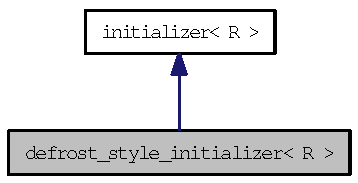
\includegraphics[width=244pt]{classdefrost__style__initializer__inherit__graph}
\end{center}
\end{figure}


Collaboration diagram for defrost\_\-style\_\-initializer$<$ R $>$:
\nopagebreak
\begin{figure}[H]
\begin{center}
\leavevmode
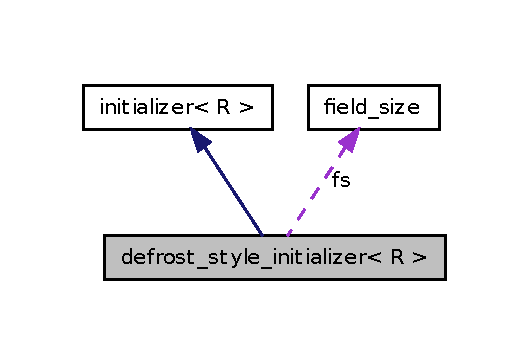
\includegraphics[width=254pt]{classdefrost__style__initializer__coll__graph}
\end{center}
\end{figure}
\subsection*{Public Member Functions}
\begin{DoxyCompactItemize}
\item 
\hypertarget{classdefrost__style__initializer_aa2a1cc1ebdd76c14d97bb63b155dee7f}{
{\bfseries defrost\_\-style\_\-initializer} (\hyperlink{structfield__size}{field\_\-size} \&fs\_\-, \hyperlink{structmodel__params}{model\_\-params}$<$ R $>$ \&mp\_\-, \hyperlink{classfield}{field}$<$ R $>$ \&phi\_\-, \hyperlink{classfield}{field}$<$ R $>$ \&phidot\_\-, \hyperlink{classfield}{field}$<$ R $>$ \&chi\_\-, \hyperlink{classfield}{field}$<$ R $>$ \&chidot\_\-, R adot\_\-)}
\label{classdefrost__style__initializer_aa2a1cc1ebdd76c14d97bb63b155dee7f}

\item 
\hypertarget{classdefrost__style__initializer_a862bd10996445ab83e81caabf7f21676}{
virtual void \hyperlink{classdefrost__style__initializer_a862bd10996445ab83e81caabf7f21676}{initialize} ()}
\label{classdefrost__style__initializer_a862bd10996445ab83e81caabf7f21676}

\begin{DoxyCompactList}\small\item\em Initialize the phi, phidot, chi and chidot fields. \item\end{DoxyCompactList}\end{DoxyCompactItemize}
\subsection*{Protected Member Functions}
\begin{DoxyCompactItemize}
\item 
void \hyperlink{classdefrost__style__initializer_a37b1d166d031097073140552513bc132}{sample\_\-grf} (\hyperlink{classfield}{field}$<$ R $>$ \&fld, R gamma, R m2eff)
\begin{DoxyCompactList}\small\item\em Sample a Gaussian random field. \item\end{DoxyCompactList}\end{DoxyCompactItemize}
\subsection*{Protected Attributes}
\begin{DoxyCompactItemize}
\item 
\hypertarget{classdefrost__style__initializer_a685da95d63057c41972961f82b1c7f8e}{
\hyperlink{structfield__size}{field\_\-size} \& {\bfseries fs}}
\label{classdefrost__style__initializer_a685da95d63057c41972961f82b1c7f8e}

\item 
\hypertarget{classdefrost__style__initializer_a02db3328866900fc1d54e419e4d0f9e1}{
\hyperlink{structmodel__params}{model\_\-params}$<$ R $>$ \& {\bfseries mp}}
\label{classdefrost__style__initializer_a02db3328866900fc1d54e419e4d0f9e1}

\item 
\hypertarget{classdefrost__style__initializer_a11f22b34b8b64a1b17c809afbfb65f3b}{
\hyperlink{classfield}{field}$<$ R $>$ \& {\bfseries phi}}
\label{classdefrost__style__initializer_a11f22b34b8b64a1b17c809afbfb65f3b}

\item 
\hypertarget{classdefrost__style__initializer_a27a44a23c3b13965cbb0eedfd585c835}{
\hyperlink{classfield}{field}$<$ R $>$ \& {\bfseries phidot}}
\label{classdefrost__style__initializer_a27a44a23c3b13965cbb0eedfd585c835}

\item 
\hypertarget{classdefrost__style__initializer_a50d49a930e6fa3679ba613136b57e36a}{
\hyperlink{classfield}{field}$<$ R $>$ \& {\bfseries chi}}
\label{classdefrost__style__initializer_a50d49a930e6fa3679ba613136b57e36a}

\item 
\hypertarget{classdefrost__style__initializer_a0a593b6c1db46eae370a21cc88b89c23}{
\hyperlink{classfield}{field}$<$ R $>$ \& {\bfseries chidot}}
\label{classdefrost__style__initializer_a0a593b6c1db46eae370a21cc88b89c23}

\item 
\hypertarget{classdefrost__style__initializer_a218c42e966ea3eb4abd8d71d7a31d4e7}{
R {\bfseries adot}}
\label{classdefrost__style__initializer_a218c42e966ea3eb4abd8d71d7a31d4e7}

\end{DoxyCompactItemize}


\subsection{Detailed Description}
\subsubsection*{template$<$typename R$>$ class defrost\_\-style\_\-initializer$<$ R $>$}

DEFROST-\/style initial conditions. 

\subsection{Member Function Documentation}
\hypertarget{classdefrost__style__initializer_a37b1d166d031097073140552513bc132}{
\index{defrost\_\-style\_\-initializer@{defrost\_\-style\_\-initializer}!sample\_\-grf@{sample\_\-grf}}
\index{sample\_\-grf@{sample\_\-grf}!defrost_style_initializer@{defrost\_\-style\_\-initializer}}
\subsubsection[{sample\_\-grf}]{\setlength{\rightskip}{0pt plus 5cm}template$<$typename R $>$ void {\bf defrost\_\-style\_\-initializer}$<$ R $>$::sample\_\-grf (
\begin{DoxyParamCaption}
\item[{{\bf field}$<$ R $>$ \&}]{ fld, }
\item[{R}]{ gamma, }
\item[{R}]{ m2eff}
\end{DoxyParamCaption}
)\hspace{0.3cm}{\ttfamily  \mbox{[}protected\mbox{]}}}}
\label{classdefrost__style__initializer_a37b1d166d031097073140552513bc132}


Sample a Gaussian random field. 

Random Gaussian-\/mode amplitudes $b_k$ are chosen such that $<b_k b^*_{k'}> = \delta(k - k')$ using the Box-\/Muller transformation. The kernel function is defined as: \[ \zeta(r) = \frac{1}{\sqrt{\pi}} \int dk \, k^2 (k^2 + m_{\mbox{eff}})^\gamma \frac{\sin(kr)}{kr} e^{-k^2/q^2} \]

$q$ is chosen to be some scale below the Nyquist frequency.


\begin{DoxyParams}{Parameters}
\item[{\em fld}]The field into which to store the random field sample. \item[{\em gamma}]The $(k^2 + m^2)$ exponent. \item[{\em m2eff}]The effective mass. \end{DoxyParams}


References field$<$ R $>$::data, field$<$ R $>$::ldl, and field$<$ R $>$::mdata.



Referenced by defrost\_\-style\_\-initializer$<$ R $>$::initialize().



The documentation for this class was generated from the following files:\begin{DoxyCompactItemize}
\item 
\hyperlink{defrost__style__initializer_8hpp}{defrost\_\-style\_\-initializer.hpp}\item 
defrost\_\-style\_\-initializer.cpp\end{DoxyCompactItemize}

\hypertarget{classenergy__outputter}{
\section{energy\_\-outputter$<$ R $>$ Class Template Reference}
\label{classenergy__outputter}\index{energy\_\-outputter@{energy\_\-outputter}}
}


Outputter for the energy TSV file.  


{\ttfamily \#include $<$energy\_\-outputter.hpp$>$}Collaboration diagram for energy\_\-outputter$<$ R $>$:\nopagebreak
\begin{figure}[H]
\begin{center}
\leavevmode
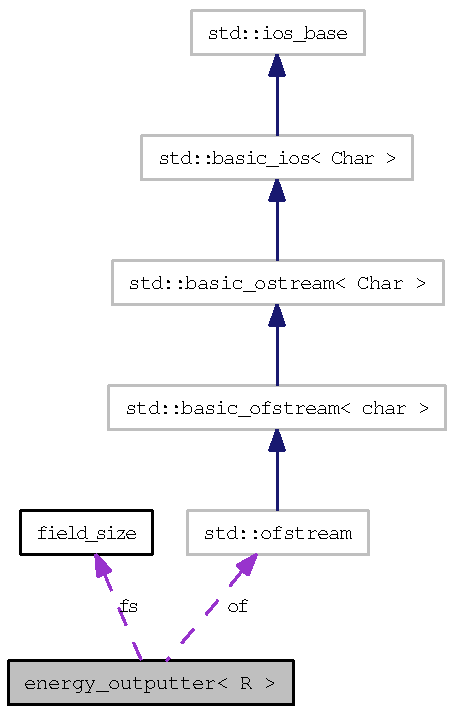
\includegraphics[width=254pt]{classenergy__outputter__coll__graph}
\end{center}
\end{figure}
\subsection*{Public Member Functions}
\begin{DoxyCompactItemize}
\item 
\hypertarget{classenergy__outputter_aa0fa67cec7d405890909d6b600d81508}{
{\bfseries energy\_\-outputter} (\hyperlink{structfield__size}{field\_\-size} \&fs\_\-, \hyperlink{structmodel__params}{model\_\-params}$<$ R $>$ \&mp\_\-, \hyperlink{structtime__state}{time\_\-state}$<$ R $>$ \&ts\_\-, \hyperlink{classfield}{field}$<$ R $>$ \&phi\_\-, \hyperlink{classfield}{field}$<$ R $>$ \&chi\_\-, \hyperlink{classfield}{field}$<$ R $>$ \&phidot\_\-, \hyperlink{classfield}{field}$<$ R $>$ \&chidot\_\-)}
\label{classenergy__outputter_aa0fa67cec7d405890909d6b600d81508}

\item 
void \hyperlink{classenergy__outputter_a51f379bb757589ecf32a074227005c2c}{output} (bool no\_\-output=false)
\begin{DoxyCompactList}\small\item\em Compute the integrated energy density and write it to the file. \item\end{DoxyCompactList}\end{DoxyCompactItemize}
\subsection*{Public Attributes}
\begin{DoxyCompactItemize}
\item 
\hypertarget{classenergy__outputter_ac58a42c4899705ea45ca4b4652203525}{
R \hyperlink{classenergy__outputter_ac58a42c4899705ea45ca4b4652203525}{avg\_\-rho\_\-phys}}
\label{classenergy__outputter_ac58a42c4899705ea45ca4b4652203525}

\begin{DoxyCompactList}\small\item\em The average energy density in physical units. \item\end{DoxyCompactList}\item 
\hypertarget{classenergy__outputter_ac9eefd9359cad3b1a16c829c9d5a8455}{
R \hyperlink{classenergy__outputter_ac9eefd9359cad3b1a16c829c9d5a8455}{avg\_\-rho}}
\label{classenergy__outputter_ac9eefd9359cad3b1a16c829c9d5a8455}

\begin{DoxyCompactList}\small\item\em The average energy density normalized by the Friedmann equation. \item\end{DoxyCompactList}\end{DoxyCompactItemize}
\subsection*{Protected Attributes}
\begin{DoxyCompactItemize}
\item 
\hypertarget{classenergy__outputter_ab158221fde24d51583bc88c5a27998d0}{
\hyperlink{structfield__size}{field\_\-size} \& {\bfseries fs}}
\label{classenergy__outputter_ab158221fde24d51583bc88c5a27998d0}

\item 
\hypertarget{classenergy__outputter_a33043573e3e6c9c17038b00bb0b4f2be}{
\hyperlink{structmodel__params}{model\_\-params}$<$ R $>$ \& {\bfseries mp}}
\label{classenergy__outputter_a33043573e3e6c9c17038b00bb0b4f2be}

\item 
\hypertarget{classenergy__outputter_a20ec80c25fb1145959e5311a2481c752}{
\hyperlink{structtime__state}{time\_\-state}$<$ R $>$ \& {\bfseries ts}}
\label{classenergy__outputter_a20ec80c25fb1145959e5311a2481c752}

\item 
\hypertarget{classenergy__outputter_ab19288ead97fb856120c3729fd67c1a5}{
\hyperlink{classfield}{field}$<$ R $>$ \& {\bfseries phi}}
\label{classenergy__outputter_ab19288ead97fb856120c3729fd67c1a5}

\item 
\hypertarget{classenergy__outputter_ad79e7c9d78dcf5489e2b36dc46839012}{
\hyperlink{classfield}{field}$<$ R $>$ \& {\bfseries chi}}
\label{classenergy__outputter_ad79e7c9d78dcf5489e2b36dc46839012}

\item 
\hypertarget{classenergy__outputter_abe7780be8621c4fb5c80f83dbce3553e}{
\hyperlink{classfield}{field}$<$ R $>$ \& {\bfseries phidot}}
\label{classenergy__outputter_abe7780be8621c4fb5c80f83dbce3553e}

\item 
\hypertarget{classenergy__outputter_a4767530c969dc638c6ed6963ce8e371d}{
\hyperlink{classfield}{field}$<$ R $>$ \& {\bfseries chidot}}
\label{classenergy__outputter_a4767530c969dc638c6ed6963ce8e371d}

\item 
\hypertarget{classenergy__outputter_a5f553a2d5554a7d78a311257bfa3463f}{
\hyperlink{classv__integrator}{v\_\-integrator}$<$ R $>$ {\bfseries vi}}
\label{classenergy__outputter_a5f553a2d5554a7d78a311257bfa3463f}

\item 
\hypertarget{classenergy__outputter_ac07729ebb0aedd6e64726adbe552049c}{
std::ofstream {\bfseries of}}
\label{classenergy__outputter_ac07729ebb0aedd6e64726adbe552049c}

\end{DoxyCompactItemize}


\subsection{Detailed Description}
\subsubsection*{template$<$typename R$>$ class energy\_\-outputter$<$ R $>$}

Outputter for the energy TSV file. 

\subsection{Member Function Documentation}
\hypertarget{classenergy__outputter_a51f379bb757589ecf32a074227005c2c}{
\index{energy\_\-outputter@{energy\_\-outputter}!output@{output}}
\index{output@{output}!energy_outputter@{energy\_\-outputter}}
\subsubsection[{output}]{\setlength{\rightskip}{0pt plus 5cm}template$<$typename R $>$ void {\bf energy\_\-outputter}$<$ R $>$::output (bool {\em no\_\-output} = {\ttfamily false})\hspace{0.3cm}{\ttfamily  \mbox{[}inline\mbox{]}}}}
\label{classenergy__outputter_a51f379bb757589ecf32a074227005c2c}


Compute the integrated energy density and write it to the file. 
\begin{DoxyParams}{Parameters}
\item[{\em no\_\-output}]If true the result is not output to the file. \end{DoxyParams}


References energy\_\-outputter$<$ R $>$::avg\_\-rho, and energy\_\-outputter$<$ R $>$::avg\_\-rho\_\-phys.

The documentation for this class was generated from the following files:\begin{DoxyCompactItemize}
\item 
\hyperlink{energy__outputter_8hpp}{energy\_\-outputter.hpp}\item 
energy\_\-outputter.cpp\end{DoxyCompactItemize}

\hypertarget{classfft__dft__c2r__3d__plan}{
\section{fft\_\-dft\_\-c2r\_\-3d\_\-plan$<$ R $>$ Class Template Reference}
\label{classfft__dft__c2r__3d__plan}\index{fft\_\-dft\_\-c2r\_\-3d\_\-plan@{fft\_\-dft\_\-c2r\_\-3d\_\-plan}}
}
\subsubsection*{template$<$typename R$>$ class fft\_\-dft\_\-c2r\_\-3d\_\-plan$<$ R $>$}



The documentation for this class was generated from the following file:\begin{DoxyCompactItemize}
\item 
\hyperlink{fft_8hpp}{fft.hpp}\end{DoxyCompactItemize}

\hypertarget{classfft__dft__c2r__3d__plan_3_01double_01_4}{
\section{fft\_\-dft\_\-c2r\_\-3d\_\-plan$<$ double $>$ Class Template Reference}
\label{classfft__dft__c2r__3d__plan_3_01double_01_4}\index{fft\_\-dft\_\-c2r\_\-3d\_\-plan$<$ double $>$@{fft\_\-dft\_\-c2r\_\-3d\_\-plan$<$ double $>$}}
}
\subsection*{Public Types}
\begin{DoxyCompactItemize}
\item 
\hypertarget{classfft__dft__c2r__3d__plan_3_01double_01_4_af2e1937067ca9111b75f50a02b286be6}{
typedef fftw\_\-complex {\bfseries complex\_\-t}}
\label{classfft__dft__c2r__3d__plan_3_01double_01_4_af2e1937067ca9111b75f50a02b286be6}

\end{DoxyCompactItemize}
\subsection*{Public Member Functions}
\begin{DoxyCompactItemize}
\item 
\hypertarget{classfft__dft__c2r__3d__plan_3_01double_01_4_a6b75061e8b9a7e9610286a88d39c6de2}{
{\bfseries fft\_\-dft\_\-c2r\_\-3d\_\-plan} (int n0, int n1, int n2, complex\_\-t $\ast$in, double $\ast$out, bool estimate=true)}
\label{classfft__dft__c2r__3d__plan_3_01double_01_4_a6b75061e8b9a7e9610286a88d39c6de2}

\item 
\hypertarget{classfft__dft__c2r__3d__plan_3_01double_01_4_ac8a8cf81fd7a1744c7a6cea9c6a01a4c}{
void {\bfseries construct} (int n0, int n1, int n2, complex\_\-t $\ast$in, double $\ast$out, bool estimate=true)}
\label{classfft__dft__c2r__3d__plan_3_01double_01_4_ac8a8cf81fd7a1744c7a6cea9c6a01a4c}

\item 
\hypertarget{classfft__dft__c2r__3d__plan_3_01double_01_4_ad43ba2cee93d0690a620fa5a03903c60}{
void {\bfseries execute} ()}
\label{classfft__dft__c2r__3d__plan_3_01double_01_4_ad43ba2cee93d0690a620fa5a03903c60}

\item 
\hypertarget{classfft__dft__c2r__3d__plan_3_01double_01_4_aa3af7e4915a166df7260eb72310a3869}{
bool {\bfseries constructed} ()}
\label{classfft__dft__c2r__3d__plan_3_01double_01_4_aa3af7e4915a166df7260eb72310a3869}

\end{DoxyCompactItemize}
\subsection*{Protected Attributes}
\begin{DoxyCompactItemize}
\item 
\hypertarget{classfft__dft__c2r__3d__plan_3_01double_01_4_ae019df4218f3519eea8e177592f81ad9}{
fftw\_\-plan {\bfseries plan}}
\label{classfft__dft__c2r__3d__plan_3_01double_01_4_ae019df4218f3519eea8e177592f81ad9}

\end{DoxyCompactItemize}
\subsubsection*{template$<$$>$ class fft\_\-dft\_\-c2r\_\-3d\_\-plan$<$ double $>$}



The documentation for this class was generated from the following file:\begin{DoxyCompactItemize}
\item 
\hyperlink{fft_8hpp}{fft.hpp}\end{DoxyCompactItemize}

\hypertarget{classfft__dft__r2c__3d__plan}{
\section{fft\_\-dft\_\-r2c\_\-3d\_\-plan$<$ R $>$ Class Template Reference}
\label{classfft__dft__r2c__3d__plan}\index{fft\_\-dft\_\-r2c\_\-3d\_\-plan@{fft\_\-dft\_\-r2c\_\-3d\_\-plan}}
}
\subsubsection*{template$<$typename R$>$ class fft\_\-dft\_\-r2c\_\-3d\_\-plan$<$ R $>$}



The documentation for this class was generated from the following file:\begin{DoxyCompactItemize}
\item 
\hyperlink{fft_8hpp}{fft.hpp}\end{DoxyCompactItemize}

\hypertarget{classfft__dft__r2c__3d__plan_3_01double_01_4}{
\section{fft\_\-dft\_\-r2c\_\-3d\_\-plan$<$ double $>$ Class Template Reference}
\label{classfft__dft__r2c__3d__plan_3_01double_01_4}\index{fft\_\-dft\_\-r2c\_\-3d\_\-plan$<$ double $>$@{fft\_\-dft\_\-r2c\_\-3d\_\-plan$<$ double $>$}}
}
\subsection*{Public Types}
\begin{DoxyCompactItemize}
\item 
\hypertarget{classfft__dft__r2c__3d__plan_3_01double_01_4_acb9081f5188f58c64467774b303680a0}{
typedef fftw\_\-complex {\bfseries complex\_\-t}}
\label{classfft__dft__r2c__3d__plan_3_01double_01_4_acb9081f5188f58c64467774b303680a0}

\end{DoxyCompactItemize}
\subsection*{Public Member Functions}
\begin{DoxyCompactItemize}
\item 
\hypertarget{classfft__dft__r2c__3d__plan_3_01double_01_4_af16576afef3939eb04b476a6d3589f30}{
{\bfseries fft\_\-dft\_\-r2c\_\-3d\_\-plan} (int n0, int n1, int n2, double $\ast$in, complex\_\-t $\ast$out, bool estimate=true)}
\label{classfft__dft__r2c__3d__plan_3_01double_01_4_af16576afef3939eb04b476a6d3589f30}

\item 
\hypertarget{classfft__dft__r2c__3d__plan_3_01double_01_4_acd216507da9226fbb4e2ffd9da091296}{
void {\bfseries execute} ()}
\label{classfft__dft__r2c__3d__plan_3_01double_01_4_acd216507da9226fbb4e2ffd9da091296}

\item 
\hypertarget{classfft__dft__r2c__3d__plan_3_01double_01_4_afd9465898cd469aaff98672d9b0ab4db}{
void {\bfseries construct} (int n0, int n1, int n2, double $\ast$in, complex\_\-t $\ast$out, bool estimate=true)}
\label{classfft__dft__r2c__3d__plan_3_01double_01_4_afd9465898cd469aaff98672d9b0ab4db}

\item 
\hypertarget{classfft__dft__r2c__3d__plan_3_01double_01_4_ae0568ff7f9b6f3f065a6240071c0a5d2}{
bool {\bfseries constructed} ()}
\label{classfft__dft__r2c__3d__plan_3_01double_01_4_ae0568ff7f9b6f3f065a6240071c0a5d2}

\end{DoxyCompactItemize}
\subsection*{Protected Attributes}
\begin{DoxyCompactItemize}
\item 
\hypertarget{classfft__dft__r2c__3d__plan_3_01double_01_4_a71d0a9c9d95023e8c617ea74d6a1d2b0}{
fftw\_\-plan {\bfseries plan}}
\label{classfft__dft__r2c__3d__plan_3_01double_01_4_a71d0a9c9d95023e8c617ea74d6a1d2b0}

\end{DoxyCompactItemize}
\subsubsection*{template$<$$>$ class fft\_\-dft\_\-r2c\_\-3d\_\-plan$<$ double $>$}



The documentation for this class was generated from the following file:\begin{DoxyCompactItemize}
\item 
\hyperlink{fft_8hpp}{fft.hpp}\end{DoxyCompactItemize}

\hypertarget{classfft__r2r__1d__plan}{
\section{fft\_\-r2r\_\-1d\_\-plan$<$ R $>$ Class Template Reference}
\label{classfft__r2r__1d__plan}\index{fft\_\-r2r\_\-1d\_\-plan@{fft\_\-r2r\_\-1d\_\-plan}}
}
\subsubsection*{template$<$typename R$>$ class fft\_\-r2r\_\-1d\_\-plan$<$ R $>$}



The documentation for this class was generated from the following file:\begin{DoxyCompactItemize}
\item 
\hyperlink{fft_8hpp}{fft.hpp}\end{DoxyCompactItemize}

\hypertarget{classfft__r2r__1d__plan_3_01double_01_4}{
\section{fft\_\-r2r\_\-1d\_\-plan$<$ double $>$ Class Template Reference}
\label{classfft__r2r__1d__plan_3_01double_01_4}\index{fft\_\-r2r\_\-1d\_\-plan$<$ double $>$@{fft\_\-r2r\_\-1d\_\-plan$<$ double $>$}}
}
\subsection*{Public Member Functions}
\begin{DoxyCompactItemize}
\item 
\hypertarget{classfft__r2r__1d__plan_3_01double_01_4_afd03767e1f4f271dc95bbe9f192cc4d9}{
{\bfseries fft\_\-r2r\_\-1d\_\-plan} (int n, double $\ast$in, double $\ast$out, fft\_\-r2r\_\-kind kind, bool estimate=true)}
\label{classfft__r2r__1d__plan_3_01double_01_4_afd03767e1f4f271dc95bbe9f192cc4d9}

\item 
\hypertarget{classfft__r2r__1d__plan_3_01double_01_4_a6eeee11780f982e75dd7bec9ad76aa9f}{
void {\bfseries construct} (int n, double $\ast$in, double $\ast$out, fft\_\-r2r\_\-kind kind, bool estimate=true)}
\label{classfft__r2r__1d__plan_3_01double_01_4_a6eeee11780f982e75dd7bec9ad76aa9f}

\item 
\hypertarget{classfft__r2r__1d__plan_3_01double_01_4_abb2a98075eb18540200066c3e81ad241}{
void {\bfseries execute} ()}
\label{classfft__r2r__1d__plan_3_01double_01_4_abb2a98075eb18540200066c3e81ad241}

\item 
\hypertarget{classfft__r2r__1d__plan_3_01double_01_4_a2bfa463f3a9531fd8996e1b61a829e50}{
bool {\bfseries constructed} ()}
\label{classfft__r2r__1d__plan_3_01double_01_4_a2bfa463f3a9531fd8996e1b61a829e50}

\end{DoxyCompactItemize}
\subsection*{Protected Attributes}
\begin{DoxyCompactItemize}
\item 
\hypertarget{classfft__r2r__1d__plan_3_01double_01_4_a23dbeca06e85dcdfaabfd00e47bcac89}{
fftw\_\-plan {\bfseries plan}}
\label{classfft__r2r__1d__plan_3_01double_01_4_a23dbeca06e85dcdfaabfd00e47bcac89}

\end{DoxyCompactItemize}
\subsubsection*{template$<$$>$ class fft\_\-r2r\_\-1d\_\-plan$<$ double $>$}



The documentation for this class was generated from the following file:\begin{DoxyCompactItemize}
\item 
\hyperlink{fft_8hpp}{fft.hpp}\end{DoxyCompactItemize}

\hypertarget{classfield}{
\section{field$<$ R $>$ Class Template Reference}
\label{classfield}\index{field@{field}}
}


A three-\/dimensional scalar field in both position and momentum space.  




{\ttfamily \#include $<$field.hpp$>$}



Collaboration diagram for field$<$ R $>$:
\nopagebreak
\begin{figure}[H]
\begin{center}
\leavevmode
\includegraphics[width=146pt]{classfield__coll__graph}
\end{center}
\end{figure}
\subsection*{Public Types}
\begin{DoxyCompactItemize}
\item 
\hypertarget{classfield_a4783d2c59b62ef73a4c3f4f7ca0b2fb7}{
typedef \hyperlink{classfft__dft__r2c__3d__plan}{fft\_\-dft\_\-r2c\_\-3d\_\-plan}$<$ R $>$::complex\_\-t {\bfseries complex\_\-t}}
\label{classfield_a4783d2c59b62ef73a4c3f4f7ca0b2fb7}

\end{DoxyCompactItemize}
\subsection*{Public Member Functions}
\begin{DoxyCompactItemize}
\item 
\hypertarget{classfield_a394818f5415834dcbc300bf5146f3357}{
{\bfseries field} (\hyperlink{structfield__size}{field\_\-size} \&fs\_\-, bool oop=false, const char $\ast$name\_\-=0)}
\label{classfield_a394818f5415834dcbc300bf5146f3357}

\item 
\hypertarget{classfield_a80228ae228b3e43f9bb04a3ab6a38a02}{
{\bfseries field} (const char $\ast$name\_\-=0)}
\label{classfield_a80228ae228b3e43f9bb04a3ab6a38a02}

\item 
\hypertarget{classfield_affd7a0214868da4208dc4bbd2ba938d4}{
void {\bfseries construct} (\hyperlink{structfield__size}{field\_\-size} \&fs\_\-, bool oop=false)}
\label{classfield_affd7a0214868da4208dc4bbd2ba938d4}

\item 
\hypertarget{classfield_a2a52cc6c193a8d2705db4eda9a96d256}{
void {\bfseries divby} (R v)}
\label{classfield_a2a52cc6c193a8d2705db4eda9a96d256}

\item 
\hypertarget{classfield_a3f6f257e24f5f6a3994c5361e84f0827}{
void {\bfseries switch\_\-state} (field\_\-state state\_\-, bool mmo=false)}
\label{classfield_a3f6f257e24f5f6a3994c5361e84f0827}

\item 
\hypertarget{classfield_a58f704053fd6528f5d80e8a3b981d4cd}{
bool {\bfseries is\_\-in\_\-place} ()}
\label{classfield_a58f704053fd6528f5d80e8a3b981d4cd}

\end{DoxyCompactItemize}
\subsection*{Public Attributes}
\begin{DoxyCompactItemize}
\item 
\hypertarget{classfield_ae4706cc48462e7ff81aace174cc02c6b}{
\hyperlink{structfield__size}{field\_\-size} {\bfseries fs}}
\label{classfield_ae4706cc48462e7ff81aace174cc02c6b}

\item 
R $\ast$ \hyperlink{classfield_a5c465fa5d00104c5bbb683a6574a4057}{data}
\begin{DoxyCompactList}\small\item\em The position-\/space data. \item\end{DoxyCompactList}\item 
\hypertarget{classfield_abab5ca89b0c6dde39ce92a372d3446bf}{
int \hyperlink{classfield_abab5ca89b0c6dde39ce92a372d3446bf}{ldl}}
\label{classfield_abab5ca89b0c6dde39ce92a372d3446bf}

\begin{DoxyCompactList}\small\item\em The length of the last dimension of the data array. \item\end{DoxyCompactList}\item 
\hypertarget{classfield_a673a06623fbbe0daf28e2406c195582e}{
int \hyperlink{classfield_a673a06623fbbe0daf28e2406c195582e}{pldl}}
\label{classfield_a673a06623fbbe0daf28e2406c195582e}

\begin{DoxyCompactList}\small\item\em The length of the last dimension of the padded data array. \item\end{DoxyCompactList}\item 
\hypertarget{classfield_a49ff854ecfe1997596a425e34964af9b}{
\hyperlink{classfft__dft__c2r__3d__plan}{fft\_\-dft\_\-c2r\_\-3d\_\-plan}$<$ R $>$::complex\_\-t $\ast$ \hyperlink{classfield_a49ff854ecfe1997596a425e34964af9b}{mdata}}
\label{classfield_a49ff854ecfe1997596a425e34964af9b}

\begin{DoxyCompactList}\small\item\em The momentum-\/space data. \item\end{DoxyCompactList}\item 
\hypertarget{classfield_a0a82ffffc6d875d5b333d48a80787cdd}{
const char $\ast$ {\bfseries name}}
\label{classfield_a0a82ffffc6d875d5b333d48a80787cdd}

\end{DoxyCompactItemize}
\subsection*{Protected Member Functions}
\begin{DoxyCompactItemize}
\item 
\hypertarget{classfield_a80741dda39b5efb7243d963bcb95dcca}{
void {\bfseries pad\_\-momentum\_\-grid} ()}
\label{classfield_a80741dda39b5efb7243d963bcb95dcca}

\item 
\hypertarget{classfield_a5a0acbcd951734bcc335b7925d8b69f2}{
void {\bfseries unpad\_\-momentum\_\-grid} ()}
\label{classfield_a5a0acbcd951734bcc335b7925d8b69f2}

\end{DoxyCompactItemize}
\subsection*{Protected Attributes}
\begin{DoxyCompactItemize}
\item 
\hypertarget{classfield_a0339f4775135e5eb7670b51fab6362d7}{
field\_\-state {\bfseries state}}
\label{classfield_a0339f4775135e5eb7670b51fab6362d7}

\item 
\hypertarget{classfield_abf982d33a1c406b4eb1f4c8c467ecf11}{
\hyperlink{classfft__dft__r2c__3d__plan}{fft\_\-dft\_\-r2c\_\-3d\_\-plan}$<$ R $>$ {\bfseries p2m\_\-plan}}
\label{classfield_abf982d33a1c406b4eb1f4c8c467ecf11}

\item 
\hypertarget{classfield_a22253ddf5199719f8d8dcd01247710ca}{
\hyperlink{classfft__dft__c2r__3d__plan}{fft\_\-dft\_\-c2r\_\-3d\_\-plan}$<$ R $>$ {\bfseries m2p\_\-plan}}
\label{classfield_a22253ddf5199719f8d8dcd01247710ca}

\item 
\hypertarget{classfield_a8e03a1aa26e2cf8030907656730da254}{
\hyperlink{classfft__dft__r2c__3d__plan}{fft\_\-dft\_\-r2c\_\-3d\_\-plan}$<$ R $>$ {\bfseries padded\_\-p2m\_\-plan}}
\label{classfield_a8e03a1aa26e2cf8030907656730da254}

\item 
\hypertarget{classfield_ab27e5897e1ad678ad2168862a1c97ca6}{
\hyperlink{classfft__dft__c2r__3d__plan}{fft\_\-dft\_\-c2r\_\-3d\_\-plan}$<$ R $>$ {\bfseries padded\_\-m2p\_\-plan}}
\label{classfield_ab27e5897e1ad678ad2168862a1c97ca6}

\item 
\hypertarget{classfield_a36ec9091d81140d37552b1d6ef673e8c}{
\hyperlink{classfft__dft__c2r__3d__plan}{fft\_\-dft\_\-c2r\_\-3d\_\-plan}$<$ R $>$::complex\_\-t $\ast$ {\bfseries mdata\_\-saved}}
\label{classfield_a36ec9091d81140d37552b1d6ef673e8c}

\end{DoxyCompactItemize}


\subsection{Detailed Description}
\subsubsection*{template$<$typename R$>$ class field$<$ R $>$}

A three-\/dimensional scalar field in both position and momentum space. 

\subsection{Member Data Documentation}
\hypertarget{classfield_a5c465fa5d00104c5bbb683a6574a4057}{
\index{field@{field}!data@{data}}
\index{data@{data}!field@{field}}
\subsubsection[{data}]{\setlength{\rightskip}{0pt plus 5cm}template$<$typename R$>$ R$\ast$ {\bf field}$<$ R $>$::{\bf data}}}
\label{classfield_a5c465fa5d00104c5bbb683a6574a4057}


The position-\/space data. 

\begin{DoxyNote}{Note}
The inner (z) dimension is padded to a size of 2$\ast$(fs.n/2+1). 
\end{DoxyNote}


Referenced by defrost\_\-style\_\-initializer$<$ R $>$::sample\_\-grf().



The documentation for this class was generated from the following files:\begin{DoxyCompactItemize}
\item 
\hyperlink{field_8hpp}{field.hpp}\item 
field.cpp\end{DoxyCompactItemize}

\hypertarget{structfield__size}{
\section{field\_\-size Struct Reference}
\label{structfield__size}\index{field\_\-size@{field\_\-size}}
}
\subsection*{Public Member Functions}
\begin{DoxyCompactItemize}
\item 
\hypertarget{structfield__size_a254e4e6981aa1ffe35ea5c1483746bfb}{
{\bfseries field\_\-size} (int n\_\-=0, int n\_\-pad\_\-factor\_\-=1)}
\label{structfield__size_a254e4e6981aa1ffe35ea5c1483746bfb}

\item 
\hypertarget{structfield__size_a6a36046bb0b1af8832c01f08a6e027d4}{
void {\bfseries calculate\_\-size\_\-totals} ()}
\label{structfield__size_a6a36046bb0b1af8832c01f08a6e027d4}

\end{DoxyCompactItemize}
\subsection*{Public Attributes}
\begin{DoxyCompactItemize}
\item 
\hypertarget{structfield__size_a1ce564998368ac36020f6f995c13a5d3}{
int {\bfseries n}}
\label{structfield__size_a1ce564998368ac36020f6f995c13a5d3}

\item 
\hypertarget{structfield__size_a0b3f5b29f65549faa2517c1bc964decb}{
int {\bfseries n\_\-pad\_\-factor}}
\label{structfield__size_a0b3f5b29f65549faa2517c1bc964decb}

\item 
\hypertarget{structfield__size_ae4d4e8fc4d86b3e2f627c4429d661199}{
int {\bfseries total\_\-gridpoints}}
\label{structfield__size_ae4d4e8fc4d86b3e2f627c4429d661199}

\item 
\hypertarget{structfield__size_a092ff1172bfd7cfa999fa468308793f0}{
int {\bfseries total\_\-padded\_\-gridpoints}}
\label{structfield__size_a092ff1172bfd7cfa999fa468308793f0}

\item 
\hypertarget{structfield__size_a65f0c4c1268e8329ece29add7b4f5839}{
int {\bfseries total\_\-momentum\_\-gridpoints}}
\label{structfield__size_a65f0c4c1268e8329ece29add7b4f5839}

\item 
\hypertarget{structfield__size_ad8a51d55670b939f7f62870ce6fa0876}{
int {\bfseries total\_\-padded\_\-momentum\_\-gridpoints}}
\label{structfield__size_ad8a51d55670b939f7f62870ce6fa0876}

\item 
\hypertarget{structfield__size_a816daef8429bcca5f5a88f68e93be903}{
int {\bfseries power\_\-length}}
\label{structfield__size_a816daef8429bcca5f5a88f68e93be903}

\end{DoxyCompactItemize}


The documentation for this struct was generated from the following file:\begin{DoxyCompactItemize}
\item 
\hyperlink{field__size_8hpp}{field\_\-size.hpp}\end{DoxyCompactItemize}

\hypertarget{classgpot__computer}{
\section{gpot\_\-computer$<$ R $>$ Class Template Reference}
\label{classgpot__computer}\index{gpot\_\-computer@{gpot\_\-computer}}
}


Computer of the gravitational potential from the energy density of the phi and chi fields.  


{\ttfamily \#include $<$gpot\_\-computer.hpp$>$}Collaboration diagram for gpot\_\-computer$<$ R $>$:\nopagebreak
\begin{figure}[H]
\begin{center}
\leavevmode
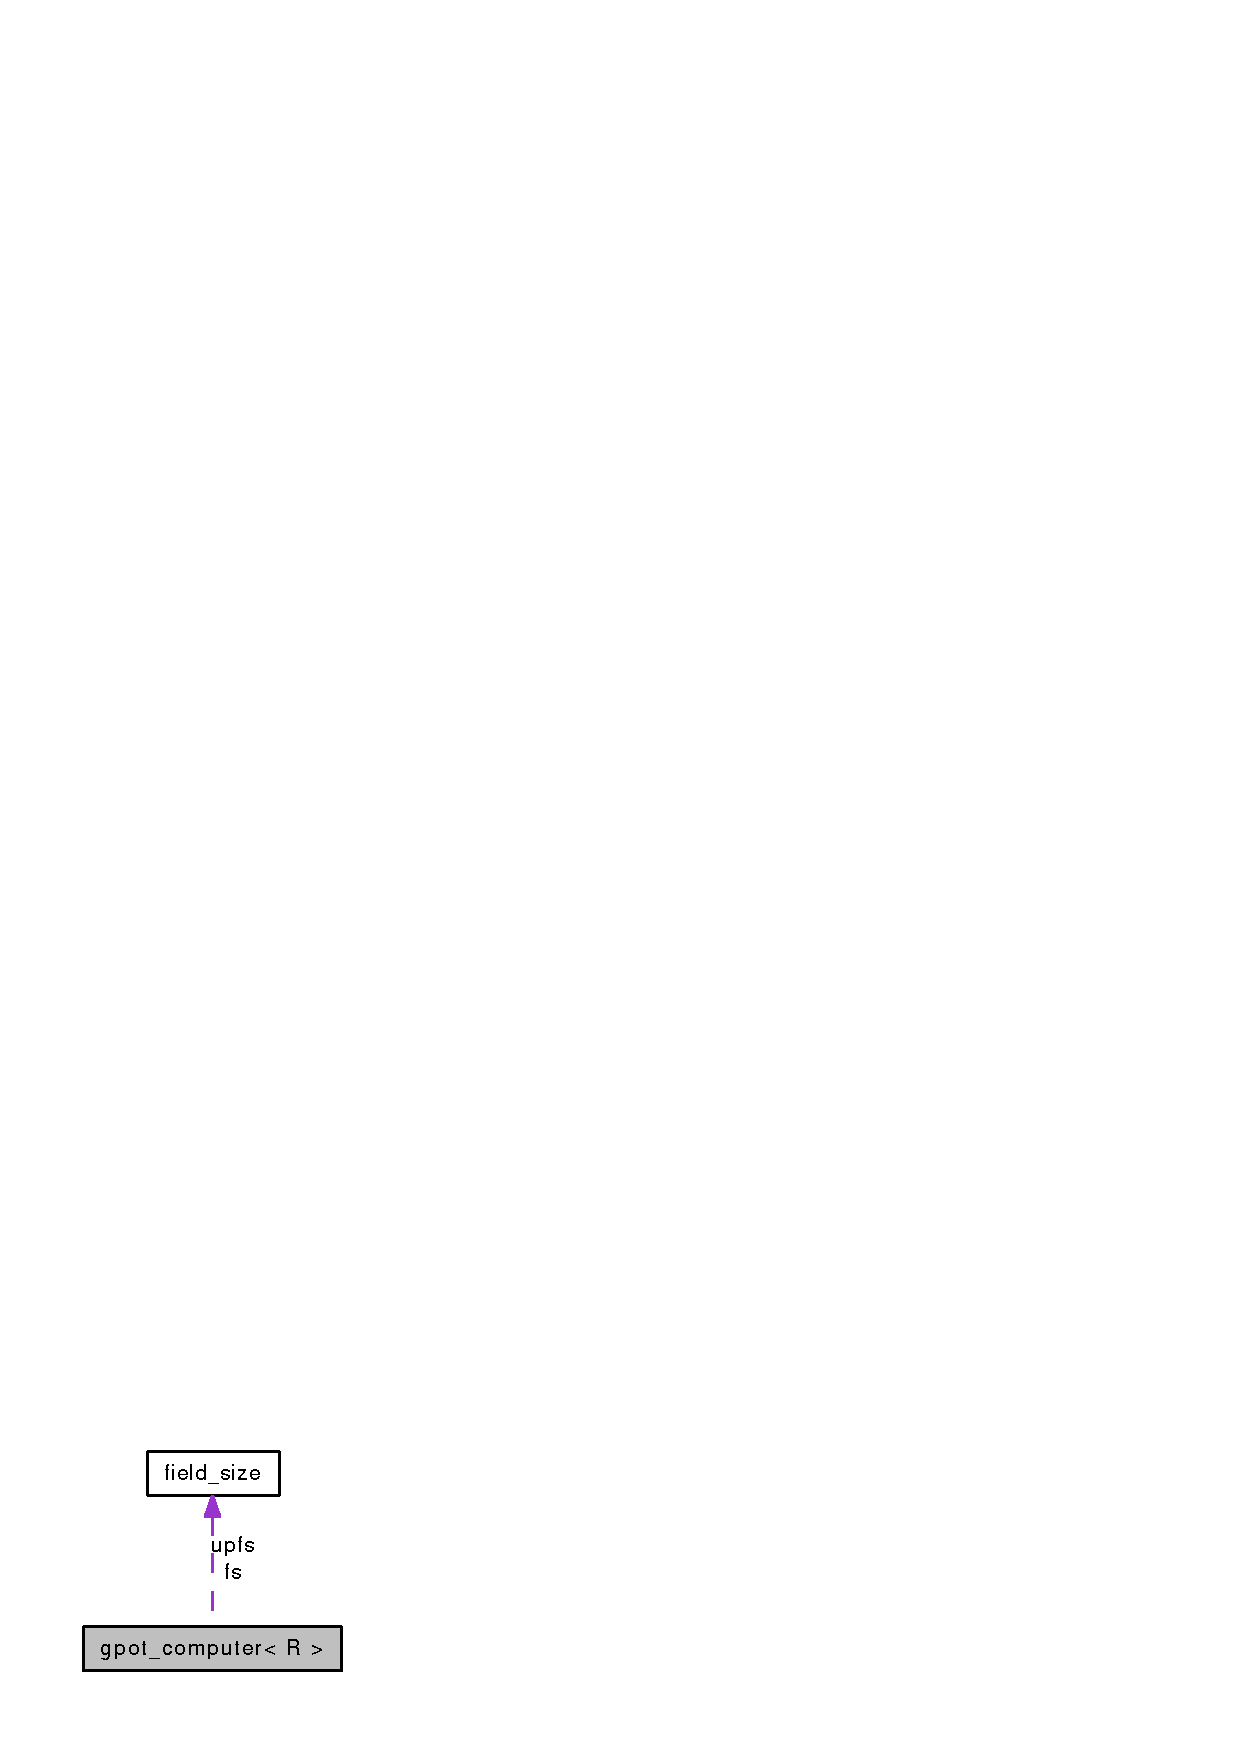
\includegraphics[width=168pt]{classgpot__computer__coll__graph}
\end{center}
\end{figure}
\subsection*{Public Member Functions}
\begin{DoxyCompactItemize}
\item 
\hypertarget{classgpot__computer_a31be021e9e6658a22bd07354e7e955a1}{
{\bfseries gpot\_\-computer} (\hyperlink{structfield__size}{field\_\-size} \&fs\_\-, \hyperlink{structmodel__params}{model\_\-params}$<$ R $>$ \&mp\_\-, \hyperlink{structtime__state}{time\_\-state}$<$ R $>$ \&ts\_\-, \hyperlink{classfield}{field}$<$ R $>$ \&phi\_\-, \hyperlink{classfield}{field}$<$ R $>$ \&chi\_\-, \hyperlink{classfield}{field}$<$ R $>$ \&phidot\_\-, \hyperlink{classfield}{field}$<$ R $>$ \&chidot\_\-, \hyperlink{classgrad__computer}{grad\_\-computer}$<$ R $>$ \&gc\_\-)}
\label{classgpot__computer_a31be021e9e6658a22bd07354e7e955a1}

\item 
void \hyperlink{classgpot__computer_adb1fb91c67e82a028c8c161007215915}{compute} (field\_\-state final\_\-state=position, bool grad\_\-computed=false)
\begin{DoxyCompactList}\small\item\em Compute gpot. \item\end{DoxyCompactList}\end{DoxyCompactItemize}
\subsection*{Public Attributes}
\begin{DoxyCompactItemize}
\item 
\hypertarget{classgpot__computer_af421e1381ed708d783c9012c4efdcb54}{
\hyperlink{classfield}{field}$<$ R $>$ \hyperlink{classgpot__computer_af421e1381ed708d783c9012c4efdcb54}{gpot}}
\label{classgpot__computer_af421e1381ed708d783c9012c4efdcb54}

\begin{DoxyCompactList}\small\item\em The gravitational potential field. \item\end{DoxyCompactList}\end{DoxyCompactItemize}
\subsection*{Protected Attributes}
\begin{DoxyCompactItemize}
\item 
\hypertarget{classgpot__computer_a5c50ce30185dfa325c019c45d75466e7}{
\hyperlink{structfield__size}{field\_\-size} \& {\bfseries fs}}
\label{classgpot__computer_a5c50ce30185dfa325c019c45d75466e7}

\item 
\hypertarget{classgpot__computer_a7401742f10b1e94290093f90bbc138f0}{
\hyperlink{structfield__size}{field\_\-size} {\bfseries upfs}}
\label{classgpot__computer_a7401742f10b1e94290093f90bbc138f0}

\item 
\hypertarget{classgpot__computer_af78203b6f7cad7aee0c181caf21fba9d}{
\hyperlink{structmodel__params}{model\_\-params}$<$ R $>$ \& {\bfseries mp}}
\label{classgpot__computer_af78203b6f7cad7aee0c181caf21fba9d}

\item 
\hypertarget{classgpot__computer_ad974327de8b6a591f239e7607ca70a46}{
\hyperlink{structtime__state}{time\_\-state}$<$ R $>$ \& {\bfseries ts}}
\label{classgpot__computer_ad974327de8b6a591f239e7607ca70a46}

\item 
\hypertarget{classgpot__computer_a335b053ba964f23aeddea3851a29179d}{
\hyperlink{classfield}{field}$<$ R $>$ \& {\bfseries phi}}
\label{classgpot__computer_a335b053ba964f23aeddea3851a29179d}

\item 
\hypertarget{classgpot__computer_ad1b3b3f9ba93ade8366471a96e91884b}{
\hyperlink{classfield}{field}$<$ R $>$ \& {\bfseries chi}}
\label{classgpot__computer_ad1b3b3f9ba93ade8366471a96e91884b}

\item 
\hypertarget{classgpot__computer_aceb973616c9b9c7f6b594296f15acfdc}{
\hyperlink{classfield}{field}$<$ R $>$ \& {\bfseries phidot}}
\label{classgpot__computer_aceb973616c9b9c7f6b594296f15acfdc}

\item 
\hypertarget{classgpot__computer_a083b742d02f75cc5c7df3ac5b63b74a6}{
\hyperlink{classfield}{field}$<$ R $>$ \& {\bfseries chidot}}
\label{classgpot__computer_a083b742d02f75cc5c7df3ac5b63b74a6}

\item 
\hypertarget{classgpot__computer_aa65ed6e5b1ed34a037bbd9241f256a74}{
\hyperlink{classgrad__computer}{grad\_\-computer}$<$ R $>$ \& {\bfseries gc}}
\label{classgpot__computer_aa65ed6e5b1ed34a037bbd9241f256a74}

\end{DoxyCompactItemize}


\subsection{Detailed Description}
\subsubsection*{template$<$typename R$>$ class gpot\_\-computer$<$ R $>$}

Computer of the gravitational potential from the energy density of the phi and chi fields. 

\subsection{Member Function Documentation}
\hypertarget{classgpot__computer_adb1fb91c67e82a028c8c161007215915}{
\index{gpot\_\-computer@{gpot\_\-computer}!compute@{compute}}
\index{compute@{compute}!gpot_computer@{gpot\_\-computer}}
\subsubsection[{compute}]{\setlength{\rightskip}{0pt plus 5cm}template$<$typename R $>$ void {\bf gpot\_\-computer}$<$ R $>$::compute (field\_\-state {\em final\_\-state} = {\ttfamily position}, \/  bool {\em grad\_\-computed} = {\ttfamily false})\hspace{0.3cm}{\ttfamily  \mbox{[}inline\mbox{]}}}}
\label{classgpot__computer_adb1fb91c67e82a028c8c161007215915}


Compute gpot. 
\begin{DoxyParams}{Parameters}
\item[{\em final\_\-state}]The final state of gpot. \item[{\em grad\_\-computed}]True if the gradient fields have already been computed (otherwise gc.compute() is called). \end{DoxyParams}


References gpot\_\-computer$<$ R $>$::gpot.

The documentation for this class was generated from the following files:\begin{DoxyCompactItemize}
\item 
\hyperlink{gpot__computer_8hpp}{gpot\_\-computer.hpp}\item 
gpot\_\-computer.cpp\end{DoxyCompactItemize}

\hypertarget{classgrad__computer}{
\section{grad\_\-computer$<$ R $>$ Class Template Reference}
\label{classgrad__computer}\index{grad\_\-computer@{grad\_\-computer}}
}


Collaboration diagram for grad\_\-computer$<$ R $>$:
\nopagebreak
\begin{figure}[H]
\begin{center}
\leavevmode
\includegraphics[width=202pt]{classgrad__computer__coll__graph}
\end{center}
\end{figure}
\subsection*{Public Member Functions}
\begin{DoxyCompactItemize}
\item 
\hypertarget{classgrad__computer_a3ff4765a6bddc2afd7d57ed129345cb6}{
{\bfseries grad\_\-computer} (\hyperlink{structfield__size}{field\_\-size} \&fs\_\-, \hyperlink{structmodel__params}{model\_\-params}$<$ R $>$ \&mp\_\-, \hyperlink{classfield}{field}$<$ R $>$ \&phi\_\-, \hyperlink{classfield}{field}$<$ R $>$ \&chi\_\-)}
\label{classgrad__computer_a3ff4765a6bddc2afd7d57ed129345cb6}

\item 
\hypertarget{classgrad__computer_ab74609eda3c169f231d9292eb49882b0}{
void {\bfseries compute} (field\_\-state final\_\-state=position)}
\label{classgrad__computer_ab74609eda3c169f231d9292eb49882b0}

\end{DoxyCompactItemize}
\subsection*{Public Attributes}
\begin{DoxyCompactItemize}
\item 
\hypertarget{classgrad__computer_aa496d530840c407086f7d7f7774e6e88}{
\hyperlink{classfield}{field}$<$ R $>$ {\bfseries phigradx}}
\label{classgrad__computer_aa496d530840c407086f7d7f7774e6e88}

\item 
\hypertarget{classgrad__computer_a9286b1ab19c2f1fe26ecf2ade34398e2}{
\hyperlink{classfield}{field}$<$ R $>$ {\bfseries chigradx}}
\label{classgrad__computer_a9286b1ab19c2f1fe26ecf2ade34398e2}

\item 
\hypertarget{classgrad__computer_aca2ec7b2438064b05eff37e13b855f65}{
\hyperlink{classfield}{field}$<$ R $>$ {\bfseries phigrady}}
\label{classgrad__computer_aca2ec7b2438064b05eff37e13b855f65}

\item 
\hypertarget{classgrad__computer_a009c81804a524ddd6535d918304743f6}{
\hyperlink{classfield}{field}$<$ R $>$ {\bfseries chigrady}}
\label{classgrad__computer_a009c81804a524ddd6535d918304743f6}

\item 
\hypertarget{classgrad__computer_a516c7ece04683a2455e48d6758ea3ec4}{
\hyperlink{classfield}{field}$<$ R $>$ {\bfseries phigradz}}
\label{classgrad__computer_a516c7ece04683a2455e48d6758ea3ec4}

\item 
\hypertarget{classgrad__computer_ab06c1070c8a5bc15ad1492e315849757}{
\hyperlink{classfield}{field}$<$ R $>$ {\bfseries chigradz}}
\label{classgrad__computer_ab06c1070c8a5bc15ad1492e315849757}

\end{DoxyCompactItemize}
\subsection*{Protected Attributes}
\begin{DoxyCompactItemize}
\item 
\hypertarget{classgrad__computer_a02be914ad46bdf588a0cf5b8f54f3860}{
\hyperlink{structfield__size}{field\_\-size} \& {\bfseries fs}}
\label{classgrad__computer_a02be914ad46bdf588a0cf5b8f54f3860}

\item 
\hypertarget{classgrad__computer_a60e6d8a2546948edecc1abe8f9b4ae57}{
\hyperlink{structfield__size}{field\_\-size} {\bfseries upfs}}
\label{classgrad__computer_a60e6d8a2546948edecc1abe8f9b4ae57}

\item 
\hypertarget{classgrad__computer_afe05111f537cc7e39c0f5d7bd7fdb1d5}{
\hyperlink{structmodel__params}{model\_\-params}$<$ R $>$ \& {\bfseries mp}}
\label{classgrad__computer_afe05111f537cc7e39c0f5d7bd7fdb1d5}

\item 
\hypertarget{classgrad__computer_aadfbdace899f83dddc6cebcf9c783e20}{
\hyperlink{classfield}{field}$<$ R $>$ \& {\bfseries phi}}
\label{classgrad__computer_aadfbdace899f83dddc6cebcf9c783e20}

\item 
\hypertarget{classgrad__computer_a4374d2769270673dd022cf47eb4e59e9}{
\hyperlink{classfield}{field}$<$ R $>$ \& {\bfseries chi}}
\label{classgrad__computer_a4374d2769270673dd022cf47eb4e59e9}

\end{DoxyCompactItemize}
\subsubsection*{template$<$typename R$>$ class grad\_\-computer$<$ R $>$}



The documentation for this class was generated from the following files:\begin{DoxyCompactItemize}
\item 
\hyperlink{grad__computer_8hpp}{grad\_\-computer.hpp}\item 
grad\_\-computer.cpp\end{DoxyCompactItemize}

\hypertarget{structgrid__funcs}{
\section{grid\_\-funcs$<$ R $>$ Struct Template Reference}
\label{structgrid__funcs}\index{grid\_\-funcs@{grid\_\-funcs}}
}
\subsection*{Static Public Member Functions}
\begin{DoxyCompactItemize}
\item 
\hypertarget{structgrid__funcs_ae3db013f110ad8e23b38207a7e3c88c5}{
static R {\bfseries compute\_\-energy\_\-scaling} (\hyperlink{structmodel__params}{model\_\-params}$<$ R $>$ \&mp, \hyperlink{structtime__state}{time\_\-state}$<$ R $>$ \&ts)}
\label{structgrid__funcs_ae3db013f110ad8e23b38207a7e3c88c5}

\item 
\hypertarget{structgrid__funcs_ae9184a5f3f25cf912540747a6a12af5d}{
static R {\bfseries compute\_\-phi} (\hyperlink{structfield__size}{field\_\-size} \&fs, \hyperlink{structmodel__params}{model\_\-params}$<$ R $>$ \&mp, \hyperlink{structtime__state}{time\_\-state}$<$ R $>$ \&ts, R phi, R chi, R phidot, R chidot, R phigradx, R chigradx, R phigrady, R chigrady, R phigradz, R chigradz, R gpot)}
\label{structgrid__funcs_ae9184a5f3f25cf912540747a6a12af5d}

\item 
\hypertarget{structgrid__funcs_a4be6b2b34635f0b88e1ddde0107e76de}{
static R {\bfseries compute\_\-chi} (\hyperlink{structfield__size}{field\_\-size} \&fs, \hyperlink{structmodel__params}{model\_\-params}$<$ R $>$ \&mp, \hyperlink{structtime__state}{time\_\-state}$<$ R $>$ \&ts, R phi, R chi, R phidot, R chidot, R phigradx, R chigradx, R phigrady, R chigrady, R phigradz, R chigradz, R gpot)}
\label{structgrid__funcs_a4be6b2b34635f0b88e1ddde0107e76de}

\item 
\hypertarget{structgrid__funcs_acd4a897e35c94b0d9117e17657183f24}{
static R {\bfseries compute\_\-gpot} (\hyperlink{structfield__size}{field\_\-size} \&fs, \hyperlink{structmodel__params}{model\_\-params}$<$ R $>$ \&mp, \hyperlink{structtime__state}{time\_\-state}$<$ R $>$ \&ts, R phi, R chi, R phidot, R chidot, R phigradx, R chigradx, R phigrady, R chigrady, R phigradz, R chigradz, R gpot)}
\label{structgrid__funcs_acd4a897e35c94b0d9117e17657183f24}

\item 
\hypertarget{structgrid__funcs_a7885ccd2de4b13fa5f62e2a54bc024c3}{
static R {\bfseries compute\_\-V\_\-phys} (\hyperlink{structfield__size}{field\_\-size} \&fs, \hyperlink{structmodel__params}{model\_\-params}$<$ R $>$ \&mp, \hyperlink{structtime__state}{time\_\-state}$<$ R $>$ \&ts, R phi, R chi, R phidot, R chidot, R phigradx, R chigradx, R phigrady, R chigrady, R phigradz, R chigradz, R gpot)}
\label{structgrid__funcs_a7885ccd2de4b13fa5f62e2a54bc024c3}

\item 
\hypertarget{structgrid__funcs_ab66e81d76717db7a9ea1253563831fde}{
static R {\bfseries compute\_\-V} (\hyperlink{structfield__size}{field\_\-size} \&fs, \hyperlink{structmodel__params}{model\_\-params}$<$ R $>$ \&mp, \hyperlink{structtime__state}{time\_\-state}$<$ R $>$ \&ts, R phi, R chi, R phidot, R chidot, R phigradx, R chigradx, R phigrady, R chigrady, R phigradz, R chigradz, R gpot)}
\label{structgrid__funcs_ab66e81d76717db7a9ea1253563831fde}

\item 
\hypertarget{structgrid__funcs_af073a8df257142a29b92fac7fb0ec993}{
static R {\bfseries compute\_\-T\_\-phi\_\-phys} (\hyperlink{structfield__size}{field\_\-size} \&fs, \hyperlink{structmodel__params}{model\_\-params}$<$ R $>$ \&mp, \hyperlink{structtime__state}{time\_\-state}$<$ R $>$ \&ts, R phi, R chi, R phidot, R chidot, R phigradx, R chigradx, R phigrady, R chigrady, R phigradz, R chigradz, R gpot)}
\label{structgrid__funcs_af073a8df257142a29b92fac7fb0ec993}

\item 
\hypertarget{structgrid__funcs_aacdcb65b1a377908aa13b2af20fb1d4a}{
static R {\bfseries compute\_\-T\_\-phi} (\hyperlink{structfield__size}{field\_\-size} \&fs, \hyperlink{structmodel__params}{model\_\-params}$<$ R $>$ \&mp, \hyperlink{structtime__state}{time\_\-state}$<$ R $>$ \&ts, R phi, R chi, R phidot, R chidot, R phigradx, R chigradx, R phigrady, R chigrady, R phigradz, R chigradz, R gpot)}
\label{structgrid__funcs_aacdcb65b1a377908aa13b2af20fb1d4a}

\item 
\hypertarget{structgrid__funcs_a0d8a5ce997dcb955a54e960f803aa0bb}{
static R {\bfseries compute\_\-T\_\-chi\_\-phys} (\hyperlink{structfield__size}{field\_\-size} \&fs, \hyperlink{structmodel__params}{model\_\-params}$<$ R $>$ \&mp, \hyperlink{structtime__state}{time\_\-state}$<$ R $>$ \&ts, R phi, R chi, R phidot, R chidot, R phigradx, R chigradx, R phigrady, R chigrady, R phigradz, R chigradz, R gpot)}
\label{structgrid__funcs_a0d8a5ce997dcb955a54e960f803aa0bb}

\item 
\hypertarget{structgrid__funcs_ae68b8f6ac20a9625b29a39f6e59d6f7d}{
static R {\bfseries compute\_\-T\_\-chi} (\hyperlink{structfield__size}{field\_\-size} \&fs, \hyperlink{structmodel__params}{model\_\-params}$<$ R $>$ \&mp, \hyperlink{structtime__state}{time\_\-state}$<$ R $>$ \&ts, R phi, R chi, R phidot, R chidot, R phigradx, R chigradx, R phigrady, R chigrady, R phigradz, R chigradz, R gpot)}
\label{structgrid__funcs_ae68b8f6ac20a9625b29a39f6e59d6f7d}

\item 
\hypertarget{structgrid__funcs_a7dd6710638fa2f82c38c33ee91a88e74}{
static R {\bfseries compute\_\-G\_\-phi\_\-phys} (\hyperlink{structfield__size}{field\_\-size} \&fs, \hyperlink{structmodel__params}{model\_\-params}$<$ R $>$ \&mp, \hyperlink{structtime__state}{time\_\-state}$<$ R $>$ \&ts, R phi, R chi, R phidot, R chidot, R phigradx, R chigradx, R phigrady, R chigrady, R phigradz, R chigradz, R gpot)}
\label{structgrid__funcs_a7dd6710638fa2f82c38c33ee91a88e74}

\item 
\hypertarget{structgrid__funcs_a007630f31ee559741783aa0a007641df}{
static R {\bfseries compute\_\-G\_\-phi} (\hyperlink{structfield__size}{field\_\-size} \&fs, \hyperlink{structmodel__params}{model\_\-params}$<$ R $>$ \&mp, \hyperlink{structtime__state}{time\_\-state}$<$ R $>$ \&ts, R phi, R chi, R phidot, R chidot, R phigradx, R chigradx, R phigrady, R chigrady, R phigradz, R chigradz, R gpot)}
\label{structgrid__funcs_a007630f31ee559741783aa0a007641df}

\item 
\hypertarget{structgrid__funcs_a517079423086048162b1f9eba0c140e1}{
static R {\bfseries compute\_\-G\_\-chi\_\-phys} (\hyperlink{structfield__size}{field\_\-size} \&fs, \hyperlink{structmodel__params}{model\_\-params}$<$ R $>$ \&mp, \hyperlink{structtime__state}{time\_\-state}$<$ R $>$ \&ts, R phi, R chi, R phidot, R chidot, R phigradx, R chigradx, R phigrady, R chigrady, R phigradz, R chigradz, R gpot)}
\label{structgrid__funcs_a517079423086048162b1f9eba0c140e1}

\item 
\hypertarget{structgrid__funcs_a83a9815afe5d0f3db972f3397598dac8}{
static R {\bfseries compute\_\-G\_\-chi} (\hyperlink{structfield__size}{field\_\-size} \&fs, \hyperlink{structmodel__params}{model\_\-params}$<$ R $>$ \&mp, \hyperlink{structtime__state}{time\_\-state}$<$ R $>$ \&ts, R phi, R chi, R phidot, R chidot, R phigradx, R chigradx, R phigrady, R chigrady, R phigradz, R chigradz, R gpot)}
\label{structgrid__funcs_a83a9815afe5d0f3db972f3397598dac8}

\item 
\hypertarget{structgrid__funcs_ac4df165d371e6e6a389d165ac4586644}{
static R {\bfseries compute\_\-rho\_\-phys} (\hyperlink{structfield__size}{field\_\-size} \&fs, \hyperlink{structmodel__params}{model\_\-params}$<$ R $>$ \&mp, \hyperlink{structtime__state}{time\_\-state}$<$ R $>$ \&ts, R phi, R chi, R phidot, R chidot, R phigradx, R chigradx, R phigrady, R chigrady, R phigradz, R chigradz, R gpot)}
\label{structgrid__funcs_ac4df165d371e6e6a389d165ac4586644}

\item 
\hypertarget{structgrid__funcs_ad043dc382653a8a220ab034304fa20c4}{
static R {\bfseries compute\_\-rho} (\hyperlink{structfield__size}{field\_\-size} \&fs, \hyperlink{structmodel__params}{model\_\-params}$<$ R $>$ \&mp, \hyperlink{structtime__state}{time\_\-state}$<$ R $>$ \&ts, R phi, R chi, R phidot, R chidot, R phigradx, R chigradx, R phigrady, R chigrady, R phigradz, R chigradz, R gpot)}
\label{structgrid__funcs_ad043dc382653a8a220ab034304fa20c4}

\item 
\hypertarget{structgrid__funcs_a67cb4b4748f1f30c063476a4ba5dbacf}{
static R {\bfseries compute\_\-p\_\-phys} (\hyperlink{structfield__size}{field\_\-size} \&fs, \hyperlink{structmodel__params}{model\_\-params}$<$ R $>$ \&mp, \hyperlink{structtime__state}{time\_\-state}$<$ R $>$ \&ts, R phi, R chi, R phidot, R chidot, R phigradx, R chigradx, R phigrady, R chigrady, R phigradz, R chigradz, R gpot)}
\label{structgrid__funcs_a67cb4b4748f1f30c063476a4ba5dbacf}

\item 
\hypertarget{structgrid__funcs_a354bdaa015579f869fa06af4b3c90039}{
static R {\bfseries compute\_\-p} (\hyperlink{structfield__size}{field\_\-size} \&fs, \hyperlink{structmodel__params}{model\_\-params}$<$ R $>$ \&mp, \hyperlink{structtime__state}{time\_\-state}$<$ R $>$ \&ts, R phi, R chi, R phidot, R chidot, R phigradx, R chigradx, R phigrady, R chigrady, R phigradz, R chigradz, R gpot)}
\label{structgrid__funcs_a354bdaa015579f869fa06af4b3c90039}

\end{DoxyCompactItemize}
\subsubsection*{template$<$typename R$>$ struct grid\_\-funcs$<$ R $>$}



The documentation for this struct was generated from the following files:\begin{DoxyCompactItemize}
\item 
\hyperlink{grid__funcs_8hpp}{grid\_\-funcs.hpp}\item 
grid\_\-funcs.cpp\end{DoxyCompactItemize}

\hypertarget{classinitializer}{
\section{initializer$<$ R $>$ Class Template Reference}
\label{classinitializer}\index{initializer@{initializer}}
}


Inheritance diagram for initializer$<$ R $>$:
\nopagebreak
\begin{figure}[H]
\begin{center}
\leavevmode
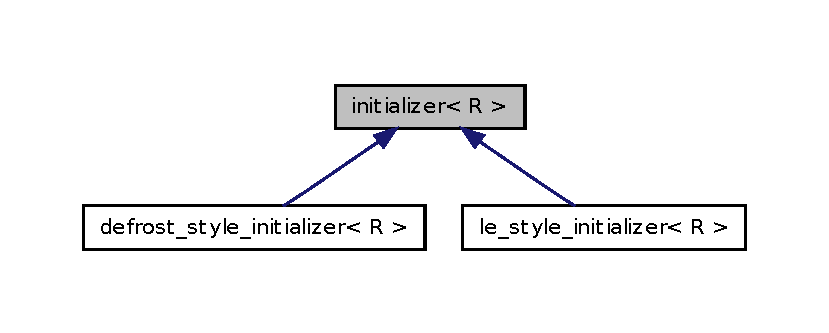
\includegraphics[width=398pt]{classinitializer__inherit__graph}
\end{center}
\end{figure}
\subsection*{Public Member Functions}
\begin{DoxyCompactItemize}
\item 
\hypertarget{classinitializer_a2d4f4facf21abb93ad032dd51c77e082}{
virtual void {\bfseries initialize} ()=0}
\label{classinitializer_a2d4f4facf21abb93ad032dd51c77e082}

\end{DoxyCompactItemize}
\subsubsection*{template$<$typename R$>$ class initializer$<$ R $>$}



The documentation for this class was generated from the following file:\begin{DoxyCompactItemize}
\item 
\hyperlink{initializer_8hpp}{initializer.hpp}\end{DoxyCompactItemize}

\hypertarget{classintegrator}{
\section{integrator$<$ R $>$ Class Template Reference}
\label{classintegrator}\index{integrator@{integrator}}
}
Inheritance diagram for integrator$<$ R $>$:\nopagebreak
\begin{figure}[H]
\begin{center}
\leavevmode
\includegraphics[width=198pt]{classintegrator__inherit__graph}
\end{center}
\end{figure}
\subsection*{Public Member Functions}
\begin{DoxyCompactItemize}
\item 
\hypertarget{classintegrator_a68b2658800a1cf018d4f6149b7cea680}{
virtual void {\bfseries step} ()=0}
\label{classintegrator_a68b2658800a1cf018d4f6149b7cea680}

\item 
\hypertarget{classintegrator_a7302a82ffd83da07291636ad2b4ed706}{
virtual void {\bfseries initialize} ()=0}
\label{classintegrator_a7302a82ffd83da07291636ad2b4ed706}

\end{DoxyCompactItemize}
\subsection*{Static Public Member Functions}
\begin{DoxyCompactItemize}
\item 
\hypertarget{classintegrator_a4443fc784fb6a07ef2f3d521e53fa53f}{
static void {\bfseries avg\_\-gradients} (\hyperlink{structfield__size}{field\_\-size} \&fs, \hyperlink{structmodel__params}{model\_\-params}$<$ R $>$ \&mp, \hyperlink{classfield}{field}$<$ R $>$ \&phi, \hyperlink{classfield}{field}$<$ R $>$ \&chi, R \&avg\_\-gradient\_\-phi, R \&avg\_\-gradient\_\-chi)}
\label{classintegrator_a4443fc784fb6a07ef2f3d521e53fa53f}

\end{DoxyCompactItemize}
\subsubsection*{template$<$typename R$>$ class integrator$<$ R $>$}



The documentation for this class was generated from the following files:\begin{DoxyCompactItemize}
\item 
\hyperlink{integrator_8hpp}{integrator.hpp}\item 
integrator.cpp\end{DoxyCompactItemize}

\hypertarget{structkeyed__value}{
\section{keyed\_\-value$<$ K, V $>$ Struct Template Reference}
\label{structkeyed__value}\index{keyed\_\-value@{keyed\_\-value}}
}


Collaboration diagram for keyed\_\-value$<$ K, V $>$:
\nopagebreak
\begin{figure}[H]
\begin{center}
\leavevmode
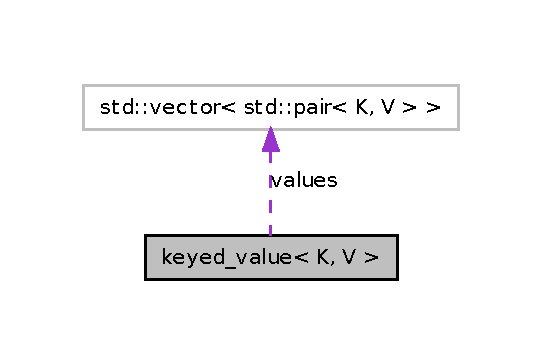
\includegraphics[width=260pt]{structkeyed__value__coll__graph}
\end{center}
\end{figure}
\subsection*{Public Member Functions}
\begin{DoxyCompactItemize}
\item 
\hypertarget{structkeyed__value_a070ede3e70ac1ab0555bf9d71d5f8c12}{
{\bfseries keyed\_\-value} (V \&v, K ik, V dv, const char $\ast$kn, const char $\ast$vn)}
\label{structkeyed__value_a070ede3e70ac1ab0555bf9d71d5f8c12}

\item 
\hypertarget{structkeyed__value_ad5f3fc8cbbc36fc6952c5bed15a22080}{
void {\bfseries advance} (K k)}
\label{structkeyed__value_ad5f3fc8cbbc36fc6952c5bed15a22080}

\item 
\hypertarget{structkeyed__value_adec20e3cf21ac1b2ad02deb5c9ede33c}{
void {\bfseries add\_\-value} (K start\_\-key, V value\_\-)}
\label{structkeyed__value_adec20e3cf21ac1b2ad02deb5c9ede33c}

\item 
\hypertarget{structkeyed__value_a7b68e8c5bb040a053c38f8a865e96daa}{
void {\bfseries finalize\_\-values} ()}
\label{structkeyed__value_a7b68e8c5bb040a053c38f8a865e96daa}

\item 
\hypertarget{structkeyed__value_a033b9d4b1f8f9b9d98ce3611a7046dc0}{
void {\bfseries summary} (std::ostream \&os)}
\label{structkeyed__value_a033b9d4b1f8f9b9d98ce3611a7046dc0}

\end{DoxyCompactItemize}
\subsection*{Public Attributes}
\begin{DoxyCompactItemize}
\item 
\hypertarget{structkeyed__value_ad9a8b0061bc126c239d11e72db9ef8ea}{
V \& {\bfseries value}}
\label{structkeyed__value_ad9a8b0061bc126c239d11e72db9ef8ea}

\item 
\hypertarget{structkeyed__value_aa2e1231c1f0adda11931eaf290d58cdf}{
const K {\bfseries initial\_\-key}}
\label{structkeyed__value_aa2e1231c1f0adda11931eaf290d58cdf}

\item 
\hypertarget{structkeyed__value_ace3c1d7bd10a09884c33ff94d3b54dee}{
const V {\bfseries default\_\-value}}
\label{structkeyed__value_ace3c1d7bd10a09884c33ff94d3b54dee}

\end{DoxyCompactItemize}
\subsection*{Protected Attributes}
\begin{DoxyCompactItemize}
\item 
\hypertarget{structkeyed__value_ad4fb83376afa71ff30330019f9c392db}{
const char $\ast$ {\bfseries key\_\-name}}
\label{structkeyed__value_ad4fb83376afa71ff30330019f9c392db}

\item 
\hypertarget{structkeyed__value_aa9010fbc96f2747c43b1778c09582ccd}{
const char $\ast$ {\bfseries value\_\-name}}
\label{structkeyed__value_aa9010fbc96f2747c43b1778c09582ccd}

\item 
\hypertarget{structkeyed__value_ad5b0261c6ecd3083c536968e66cc7221}{
std::vector$<$ std::pair$<$ K, V $>$ $>$ {\bfseries values}}
\label{structkeyed__value_ad5b0261c6ecd3083c536968e66cc7221}

\end{DoxyCompactItemize}
\subsubsection*{template$<$typename K, typename V$>$ struct keyed\_\-value$<$ K, V $>$}



The documentation for this struct was generated from the following file:\begin{DoxyCompactItemize}
\item 
\hyperlink{time__state_8hpp}{time\_\-state.hpp}\end{DoxyCompactItemize}

\hypertarget{classle__style__initializer}{
\section{le\_\-style\_\-initializer$<$ R $>$ Class Template Reference}
\label{classle__style__initializer}\index{le\_\-style\_\-initializer@{le\_\-style\_\-initializer}}
}


Inheritance diagram for le\_\-style\_\-initializer$<$ R $>$:
\nopagebreak
\begin{figure}[H]
\begin{center}
\leavevmode
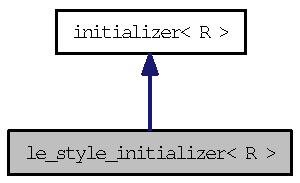
\includegraphics[width=216pt]{classle__style__initializer__inherit__graph}
\end{center}
\end{figure}


Collaboration diagram for le\_\-style\_\-initializer$<$ R $>$:
\nopagebreak
\begin{figure}[H]
\begin{center}
\leavevmode
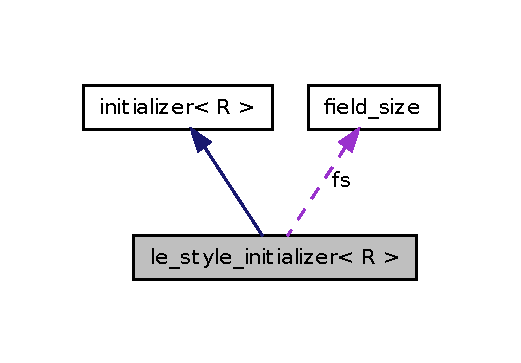
\includegraphics[width=250pt]{classle__style__initializer__coll__graph}
\end{center}
\end{figure}
\subsection*{Public Member Functions}
\begin{DoxyCompactItemize}
\item 
\hypertarget{classle__style__initializer_a7a21af6b2b39ec0800c7336b8fa47ece}{
{\bfseries le\_\-style\_\-initializer} (\hyperlink{structfield__size}{field\_\-size} \&fs\_\-, \hyperlink{structmodel__params}{model\_\-params}$<$ R $>$ \&mp\_\-, \hyperlink{classfield}{field}$<$ R $>$ \&phi\_\-, \hyperlink{classfield}{field}$<$ R $>$ \&phidot\_\-, \hyperlink{classfield}{field}$<$ R $>$ \&chi\_\-, \hyperlink{classfield}{field}$<$ R $>$ \&chidot\_\-, R adot\_\-, R len0)}
\label{classle__style__initializer_a7a21af6b2b39ec0800c7336b8fa47ece}

\item 
\hypertarget{classle__style__initializer_ac5ca8b27383d7b35170f6d5bf6e3d96f}{
virtual void {\bfseries initialize} ()}
\label{classle__style__initializer_ac5ca8b27383d7b35170f6d5bf6e3d96f}

\end{DoxyCompactItemize}
\subsection*{Protected Member Functions}
\begin{DoxyCompactItemize}
\item 
\hypertarget{classle__style__initializer_a7b95cb916de69483725ea553871a16fb}{
void {\bfseries set\_\-mode} (\hyperlink{classfield}{field}$<$ R $>$ \&fld, \hyperlink{classfield}{field}$<$ R $>$ \&flddot, R m\_\-fld\_\-eff, int px, int py, int pz, int idx, bool real=false)}
\label{classle__style__initializer_a7b95cb916de69483725ea553871a16fb}

\item 
\hypertarget{classle__style__initializer_a86624b36b749497e52835f385ecd568d}{
void {\bfseries initialize\_\-field} (\hyperlink{classfield}{field}$<$ R $>$ \&fld, \hyperlink{classfield}{field}$<$ R $>$ \&flddot, R m\_\-fld\_\-eff)}
\label{classle__style__initializer_a86624b36b749497e52835f385ecd568d}

\end{DoxyCompactItemize}
\subsection*{Protected Attributes}
\begin{DoxyCompactItemize}
\item 
\hypertarget{classle__style__initializer_a62611c6bf34270cc824bff07ae43560d}{
\hyperlink{structfield__size}{field\_\-size} \& {\bfseries fs}}
\label{classle__style__initializer_a62611c6bf34270cc824bff07ae43560d}

\item 
\hypertarget{classle__style__initializer_a73c082652784c51599ead4c6608556a7}{
\hyperlink{structmodel__params}{model\_\-params}$<$ R $>$ \& {\bfseries mp}}
\label{classle__style__initializer_a73c082652784c51599ead4c6608556a7}

\item 
\hypertarget{classle__style__initializer_a82ffd836af9e74646e87a0a8ec2b19ae}{
\hyperlink{classfield}{field}$<$ R $>$ \& {\bfseries phi}}
\label{classle__style__initializer_a82ffd836af9e74646e87a0a8ec2b19ae}

\item 
\hypertarget{classle__style__initializer_a9a1febad9cec5260d4feda55156277ba}{
\hyperlink{classfield}{field}$<$ R $>$ \& {\bfseries phidot}}
\label{classle__style__initializer_a9a1febad9cec5260d4feda55156277ba}

\item 
\hypertarget{classle__style__initializer_aac6d2b31590a8f21ffbc98a678e35c5f}{
\hyperlink{classfield}{field}$<$ R $>$ \& {\bfseries chi}}
\label{classle__style__initializer_aac6d2b31590a8f21ffbc98a678e35c5f}

\item 
\hypertarget{classle__style__initializer_afda2afd595b91480ac13655fbf3cd891}{
\hyperlink{classfield}{field}$<$ R $>$ \& {\bfseries chidot}}
\label{classle__style__initializer_afda2afd595b91480ac13655fbf3cd891}

\item 
\hypertarget{classle__style__initializer_a8023c235401ca9873ae08ab3b73cf348}{
R {\bfseries adot}}
\label{classle__style__initializer_a8023c235401ca9873ae08ab3b73cf348}

\item 
\hypertarget{classle__style__initializer_ab5113f6fdc28a74399d2ec26d8875e45}{
R {\bfseries fluctuation\_\-amplitude}}
\label{classle__style__initializer_ab5113f6fdc28a74399d2ec26d8875e45}

\end{DoxyCompactItemize}
\subsubsection*{template$<$typename R$>$ class le\_\-style\_\-initializer$<$ R $>$}



The documentation for this class was generated from the following files:\begin{DoxyCompactItemize}
\item 
\hyperlink{le__style__initializer_8hpp}{le\_\-style\_\-initializer.hpp}\item 
le\_\-style\_\-initializer.cpp\end{DoxyCompactItemize}

\hypertarget{classmodel}{
\section{model$<$ R $>$ Class Template Reference}
\label{classmodel}\index{model@{model}}
}


Collaboration diagram for model$<$ R $>$:
\nopagebreak
\begin{figure}[H]
\begin{center}
\leavevmode
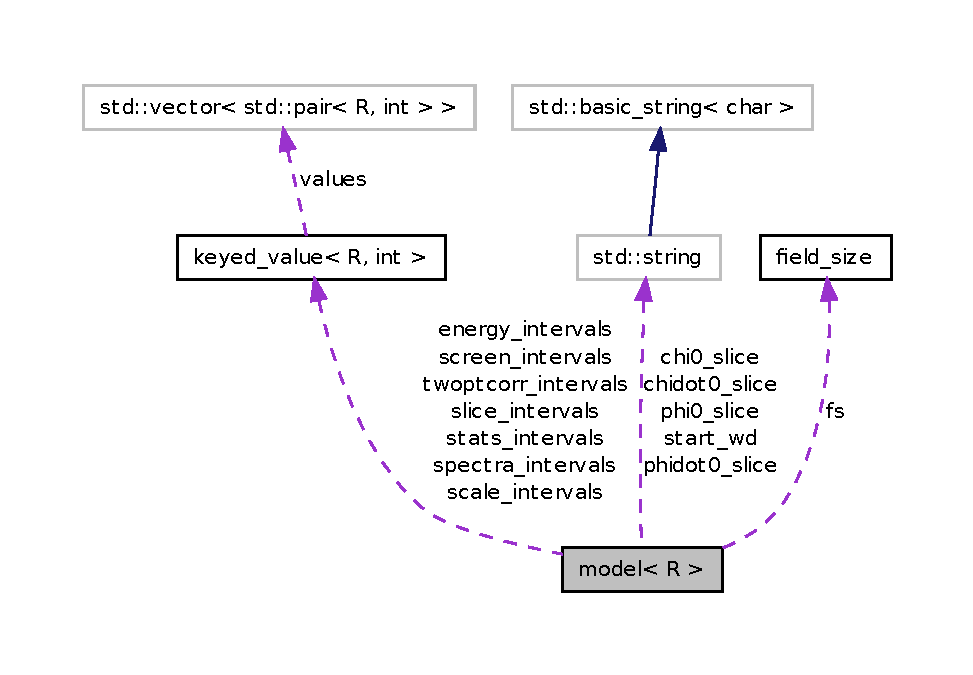
\includegraphics[width=400pt]{classmodel__coll__graph}
\end{center}
\end{figure}
\subsection*{Public Member Functions}
\begin{DoxyCompactItemize}
\item 
\hypertarget{classmodel_a1a3966e2e1ce020c9db63b11b21af282}{
{\bfseries model} (int argc, char $\ast$argv\mbox{[}$\,$\mbox{]})}
\label{classmodel_a1a3966e2e1ce020c9db63b11b21af282}

\item 
\hypertarget{classmodel_abaace1e276e1eb6010eb68049725d61d}{
void {\bfseries run} ()}
\label{classmodel_abaace1e276e1eb6010eb68049725d61d}

\end{DoxyCompactItemize}
\subsection*{Protected Member Functions}
\begin{DoxyCompactItemize}
\item 
\hypertarget{classmodel_a9d295f09eb260af90c184498422d2951}{
void {\bfseries set\_\-output\_\-directory} (const char $\ast$uodn)}
\label{classmodel_a9d295f09eb260af90c184498422d2951}

\item 
\hypertarget{classmodel_a2c46925e71c4af596e2e1ea55796d5fc}{
void {\bfseries write\_\-info\_\-file} ()}
\label{classmodel_a2c46925e71c4af596e2e1ea55796d5fc}

\item 
\hypertarget{classmodel_a26254dca4a7bb65302f8ac79ec7d880b}{
void {\bfseries set\_\-initial\_\-conditions} ()}
\label{classmodel_a26254dca4a7bb65302f8ac79ec7d880b}

\item 
\hypertarget{classmodel_a7205d404bf7eda6417fcb2162ad9baa7}{
void {\bfseries evolve} (\hyperlink{classintegrator}{integrator}$<$ R $>$ $\ast$ig)}
\label{classmodel_a7205d404bf7eda6417fcb2162ad9baa7}

\item 
\hypertarget{classmodel_aa16f656be92adeb0dc352480e343af9d}{
void {\bfseries load\_\-initial\_\-slice\_\-file} (std::string \&ifn, \hyperlink{classfield}{field}$<$ R $>$ \&fld, R pf)}
\label{classmodel_aa16f656be92adeb0dc352480e343af9d}

\item 
\hypertarget{classmodel_a3d06bc461cb157407beea8e4fd3c1182}{
void {\bfseries private\_\-allocate} ()}
\label{classmodel_a3d06bc461cb157407beea8e4fd3c1182}

\item 
\hypertarget{classmodel_a2d7c0fefd194dc3220bd155d86ebf32a}{
void {\bfseries private\_\-set\_\-sf\_\-info} ()}
\label{classmodel_a2d7c0fefd194dc3220bd155d86ebf32a}

\item 
\hypertarget{classmodel_a2112bf622835919980b9dcad666420ba}{
void {\bfseries private\_\-evolve} (int counter)}
\label{classmodel_a2112bf622835919980b9dcad666420ba}

\item 
\hypertarget{classmodel_ae729d9cc3fa9b3733523236f300e0ceb}{
void {\bfseries private\_\-info\_\-file\_\-output} (std::ofstream \&info\_\-file)}
\label{classmodel_ae729d9cc3fa9b3733523236f300e0ceb}

\end{DoxyCompactItemize}
\subsection*{Protected Attributes}
\begin{DoxyCompactItemize}
\item 
\hypertarget{classmodel_a40d2f23dcbec53f421dfa25ecc57030e}{
\hyperlink{structfield__size}{field\_\-size} {\bfseries fs}}
\label{classmodel_a40d2f23dcbec53f421dfa25ecc57030e}

\item 
\hypertarget{classmodel_aa239be849b91caa21352765567ef584a}{
\hyperlink{structmodel__params}{model\_\-params}$<$ R $>$ {\bfseries mp}}
\label{classmodel_aa239be849b91caa21352765567ef584a}

\item 
\hypertarget{classmodel_a7147930cb35a8f2aa47c4cfdc6d39c36}{
\hyperlink{structtime__state}{time\_\-state}$<$ R $>$ {\bfseries ts}}
\label{classmodel_a7147930cb35a8f2aa47c4cfdc6d39c36}

\item 
\hypertarget{classmodel_a9854a29ea87651d1ded6ca6c8790eb9b}{
bool {\bfseries use\_\-verlet}}
\label{classmodel_a9854a29ea87651d1ded6ca6c8790eb9b}

\item 
\hypertarget{classmodel_a3c6584aee08a90b08d8a5cc7d90e3a66}{
bool {\bfseries le\_\-init}}
\label{classmodel_a3c6584aee08a90b08d8a5cc7d90e3a66}

\item 
\hypertarget{classmodel_a92b75cf1df91519d2bf5a0659ad0d3b5}{
bool {\bfseries homo\_\-ic\_\-phi}}
\label{classmodel_a92b75cf1df91519d2bf5a0659ad0d3b5}

\item 
\hypertarget{classmodel_aeabac8cb1644e33a1d5db116debdf527}{
bool {\bfseries homo\_\-ic\_\-chi}}
\label{classmodel_aeabac8cb1644e33a1d5db116debdf527}

\item 
\hypertarget{classmodel_a111ad89eea9df0a5f40d30241f5884fa}{
int {\bfseries seed}}
\label{classmodel_a111ad89eea9df0a5f40d30241f5884fa}

\item 
\hypertarget{classmodel_a036cddd403fb7afcfaa62d909bba1a1b}{
R {\bfseries tf}}
\label{classmodel_a036cddd403fb7afcfaa62d909bba1a1b}

\item 
\hypertarget{classmodel_adaf2c0ea292512a3b0ad7b3eded33a38}{
int {\bfseries scale\_\-interval}}
\label{classmodel_adaf2c0ea292512a3b0ad7b3eded33a38}

\item 
\hypertarget{classmodel_abb1fa70dcb164b154962239d89549bba}{
int {\bfseries energy\_\-interval}}
\label{classmodel_abb1fa70dcb164b154962239d89549bba}

\item 
\hypertarget{classmodel_a6034345aff4e730e2d134fe4747173b3}{
int {\bfseries spectra\_\-interval}}
\label{classmodel_a6034345aff4e730e2d134fe4747173b3}

\item 
\hypertarget{classmodel_a6c573a2fe4aaed01e1f2fcde9f1228df}{
int {\bfseries screen\_\-interval}}
\label{classmodel_a6c573a2fe4aaed01e1f2fcde9f1228df}

\item 
\hypertarget{classmodel_a9561d067a967f20b946b94a2305d5501}{
int {\bfseries slice\_\-interval}}
\label{classmodel_a9561d067a967f20b946b94a2305d5501}

\item 
\hypertarget{classmodel_a5e477d9d154064d70e8da87fdc363603}{
int {\bfseries stats\_\-interval}}
\label{classmodel_a5e477d9d154064d70e8da87fdc363603}

\item 
\hypertarget{classmodel_abac663e2b450708b3d26a1c90c52541c}{
int {\bfseries twoptcorr\_\-interval}}
\label{classmodel_abac663e2b450708b3d26a1c90c52541c}

\item 
\hypertarget{classmodel_a32c9cb25d74703419261a56188cf08fd}{
\hyperlink{structkeyed__value}{keyed\_\-value}$<$ R, int $>$ {\bfseries scale\_\-intervals}}
\label{classmodel_a32c9cb25d74703419261a56188cf08fd}

\item 
\hypertarget{classmodel_aa3d0b02452be0ea6301ec2f9e5c4034d}{
\hyperlink{structkeyed__value}{keyed\_\-value}$<$ R, int $>$ {\bfseries energy\_\-intervals}}
\label{classmodel_aa3d0b02452be0ea6301ec2f9e5c4034d}

\item 
\hypertarget{classmodel_a71307003ff0cf775ac1ce91ee34bd0fd}{
\hyperlink{structkeyed__value}{keyed\_\-value}$<$ R, int $>$ {\bfseries spectra\_\-intervals}}
\label{classmodel_a71307003ff0cf775ac1ce91ee34bd0fd}

\item 
\hypertarget{classmodel_a486729c11cb76cce2cd07f127de92675}{
\hyperlink{structkeyed__value}{keyed\_\-value}$<$ R, int $>$ {\bfseries screen\_\-intervals}}
\label{classmodel_a486729c11cb76cce2cd07f127de92675}

\item 
\hypertarget{classmodel_abaa2d75f66beefce1e0a7ee6ffd8793b}{
\hyperlink{structkeyed__value}{keyed\_\-value}$<$ R, int $>$ {\bfseries slice\_\-intervals}}
\label{classmodel_abaa2d75f66beefce1e0a7ee6ffd8793b}

\item 
\hypertarget{classmodel_a20b78d7409e56144005ff30d26798e7c}{
\hyperlink{structkeyed__value}{keyed\_\-value}$<$ R, int $>$ {\bfseries stats\_\-intervals}}
\label{classmodel_a20b78d7409e56144005ff30d26798e7c}

\item 
\hypertarget{classmodel_a4bcea6b6c78361ff9ec2abd62ea9bcdf}{
\hyperlink{structkeyed__value}{keyed\_\-value}$<$ R, int $>$ {\bfseries twoptcorr\_\-intervals}}
\label{classmodel_a4bcea6b6c78361ff9ec2abd62ea9bcdf}

\item 
\hypertarget{classmodel_ae4eadf04cea985864f0fe3bc488aac5f}{
\hyperlink{classfield}{field}$<$ R $>$ {\bfseries phi}}
\label{classmodel_ae4eadf04cea985864f0fe3bc488aac5f}

\item 
\hypertarget{classmodel_a39a3d7f259f021693157b6b2d8a17285}{
\hyperlink{classfield}{field}$<$ R $>$ {\bfseries phidot}}
\label{classmodel_a39a3d7f259f021693157b6b2d8a17285}

\item 
\hypertarget{classmodel_aea7e2cf8648a963f20295d375bb3ad6b}{
\hyperlink{classfield}{field}$<$ R $>$ {\bfseries chi}}
\label{classmodel_aea7e2cf8648a963f20295d375bb3ad6b}

\item 
\hypertarget{classmodel_aeb232ddca67d5c55388e4e40f2a337c8}{
\hyperlink{classfield}{field}$<$ R $>$ {\bfseries chidot}}
\label{classmodel_aeb232ddca67d5c55388e4e40f2a337c8}

\item 
\hypertarget{classmodel_abbd490806cef7af3fb1c201190854451}{
\hyperlink{classgrad__computer}{grad\_\-computer}$<$ R $>$ $\ast$ {\bfseries gc}}
\label{classmodel_abbd490806cef7af3fb1c201190854451}

\item 
\hypertarget{classmodel_a0e84b2e244bbfaf6355a9dcfa558f860}{
\hyperlink{classgpot__computer}{gpot\_\-computer}$<$ R $>$ $\ast$ {\bfseries gpotc}}
\label{classmodel_a0e84b2e244bbfaf6355a9dcfa558f860}

\item 
\hypertarget{classmodel_ac0f228a8a23b4afaea409a0295efc73a}{
\hyperlink{classslice__output__manager}{slice\_\-output\_\-manager}$<$ R $>$ $\ast$ {\bfseries som}}
\label{classmodel_ac0f228a8a23b4afaea409a0295efc73a}

\item 
\hypertarget{classmodel_adb6d67be31d8af98fa25d81213f9bc61}{
R {\bfseries ics\_\-scale}}
\label{classmodel_adb6d67be31d8af98fa25d81213f9bc61}

\item 
\hypertarget{classmodel_aef6e146814fdda23f37ec3c5e2fafc3e}{
R {\bfseries len0}}
\label{classmodel_aef6e146814fdda23f37ec3c5e2fafc3e}

\item 
\hypertarget{classmodel_a99fba28df7c61a327a81f807bab45731}{
bool {\bfseries vvwl}}
\label{classmodel_a99fba28df7c61a327a81f807bab45731}

\item 
\hypertarget{classmodel_a232f10a2703e68837cd2b7e551632f6e}{
R {\bfseries af}}
\label{classmodel_a232f10a2703e68837cd2b7e551632f6e}

\item 
\hypertarget{classmodel_a25ef09e5d42e6130a1129ae54bb9e492}{
bool {\bfseries external\_\-H0}}
\label{classmodel_a25ef09e5d42e6130a1129ae54bb9e492}

\item 
\hypertarget{classmodel_ae646b51edb2a2434b47dae381f3e89d8}{
std::string {\bfseries phi0\_\-slice}}
\label{classmodel_ae646b51edb2a2434b47dae381f3e89d8}

\item 
\hypertarget{classmodel_ac1af4ad9e5dfc5b747fc1310e7dbb539}{
std::string {\bfseries chi0\_\-slice}}
\label{classmodel_ac1af4ad9e5dfc5b747fc1310e7dbb539}

\item 
\hypertarget{classmodel_a539de22f85f9bec7cef20f336d748607}{
std::string {\bfseries phidot0\_\-slice}}
\label{classmodel_a539de22f85f9bec7cef20f336d748607}

\item 
\hypertarget{classmodel_a38d08cfb61889a77dbf8e4e4134b017d}{
std::string {\bfseries chidot0\_\-slice}}
\label{classmodel_a38d08cfb61889a77dbf8e4e4134b017d}

\item 
\hypertarget{classmodel_a5c8df3bcc830411106f51e11f51637a1}{
std::string {\bfseries start\_\-wd}}
\label{classmodel_a5c8df3bcc830411106f51e11f51637a1}

\item 
\hypertarget{classmodel_a046d1ed1160f5b32c10e97ed7c179f48}{
int {\bfseries ics\_\-eff\_\-size}}
\label{classmodel_a046d1ed1160f5b32c10e97ed7c179f48}

\item 
\hypertarget{classmodel_a4a902b5ffa20522d6fbbf74a82d4fdd6}{
R {\bfseries phidot0pr}}
\label{classmodel_a4a902b5ffa20522d6fbbf74a82d4fdd6}

\item 
\hypertarget{classmodel_a892f62f1d79750b23b715d239af22039}{
R {\bfseries chidot0pr}}
\label{classmodel_a892f62f1d79750b23b715d239af22039}

\end{DoxyCompactItemize}
\subsubsection*{template$<$typename R$>$ class model$<$ R $>$}



The documentation for this class was generated from the following files:\begin{DoxyCompactItemize}
\item 
\hyperlink{model_8hpp}{model.hpp}\item 
model.cpp\end{DoxyCompactItemize}

\hypertarget{structmodel__params}{
\section{model\_\-params$<$ R $>$ Struct Template Reference}
\label{structmodel__params}\index{model\_\-params@{model\_\-params}}
}


Static model parameters.  




{\ttfamily \#include $<$model\_\-params.hpp$>$}

\subsection*{Public Member Functions}
\begin{DoxyCompactItemize}
\item 
\hypertarget{structmodel__params_a9bcd0871ce87aa307d0df35b7e073d72}{
void {\bfseries calculate\_\-derived\_\-params} (bool report=false)}
\label{structmodel__params_a9bcd0871ce87aa307d0df35b7e073d72}

\item 
R \hyperlink{structmodel__params_a2ca88aaf39658ce4bbe31cf92654040b}{V} (R phi, R chi, R a\_\-t)
\begin{DoxyCompactList}\small\item\em Returns the value of the field potential at a point given the values of the fields at that point. \item\end{DoxyCompactList}\item 
void \hyperlink{structmodel__params_af08a5674a6b3cb272181d29483e763d9}{derivs} (R phi, R chi, R phidot, R chidot, R chi2phi, R phi2chi, R phi3, R chi3, R phi5, R chi5, R phi\_\-md, R chi\_\-md, R a\_\-t, R adot\_\-t, R addot\_\-t, R mom2, R \&dphidt, R \&dchidt, R \&dphidotdt, R \&dchidotdt)
\begin{DoxyCompactList}\small\item\em This is where the equations of motion for the fields are actually evaluated. \item\end{DoxyCompactList}\item 
\hypertarget{structmodel__params_ac1a992d6e20b7e30b1d6e2d29bbca9d5}{
R {\bfseries adoubledot\_\-pwr\_\-exp} (R t, R a\_\-t, R adot\_\-t)}
\label{structmodel__params_ac1a992d6e20b7e30b1d6e2d29bbca9d5}

\item 
R \hyperlink{structmodel__params_ad954a15177ce8ae5cc0d8304967ef772}{adoubledot} (R t, R a\_\-t, R adot\_\-t, R avg\_\-gradient\_\-phi, R avg\_\-gradient\_\-chi, R avg\_\-V)
\begin{DoxyCompactList}\small\item\em Returns the second time derivative of the scale factor in program units. \item\end{DoxyCompactList}\item 
R \hyperlink{structmodel__params_a9406f007166bc0c58dafa5f970687ba8}{adoubledot\_\-staggered} (R t, R dt, R a\_\-t, R adot\_\-t, R avg\_\-gradient\_\-phi, R avg\_\-gradient\_\-chi, R avg\_\-V)
\begin{DoxyCompactList}\small\item\em Returns the second time derivative of the scale factor in program units at a half-\/time-\/step. \item\end{DoxyCompactList}\end{DoxyCompactItemize}
\subsection*{Public Attributes}
\begin{DoxyCompactItemize}
\item 
\hypertarget{structmodel__params_a97f9ba1a4a364b7cbf76abccf3e1d2cf}{
R {\bfseries gamma\_\-phi}}
\label{structmodel__params_a97f9ba1a4a364b7cbf76abccf3e1d2cf}

\item 
\hypertarget{structmodel__params_ad0afc68b30a56a1cfeac5f58ce65294f}{
R {\bfseries gamma\_\-chi}}
\label{structmodel__params_ad0afc68b30a56a1cfeac5f58ce65294f}

\item 
\hypertarget{structmodel__params_a0965a18e0629bdccfa4c3cec769f9df1}{
R {\bfseries lambda\_\-phi}}
\label{structmodel__params_a0965a18e0629bdccfa4c3cec769f9df1}

\item 
\hypertarget{structmodel__params_af81fcd0a7180f2dbe74fa2023ed61d62}{
R {\bfseries lambda\_\-chi}}
\label{structmodel__params_af81fcd0a7180f2dbe74fa2023ed61d62}

\item 
\hypertarget{structmodel__params_af2859f1548a8db284d37ac07a208c602}{
R {\bfseries g}}
\label{structmodel__params_af2859f1548a8db284d37ac07a208c602}

\item 
\hypertarget{structmodel__params_ace1f3f2abfe269d3220ca244b9c0b260}{
R {\bfseries m\_\-phi}}
\label{structmodel__params_ace1f3f2abfe269d3220ca244b9c0b260}

\item 
\hypertarget{structmodel__params_abf3681b51e3007234a8d00b4f2222010}{
R {\bfseries m\_\-chi}}
\label{structmodel__params_abf3681b51e3007234a8d00b4f2222010}

\item 
\hypertarget{structmodel__params_ababc32d234bb52d2226fed9f115677f8}{
R {\bfseries md\_\-e\_\-phi}}
\label{structmodel__params_ababc32d234bb52d2226fed9f115677f8}

\item 
\hypertarget{structmodel__params_acd9ced3452f08a9ec45d518c7e5ca3e0}{
R {\bfseries md\_\-e\_\-chi}}
\label{structmodel__params_acd9ced3452f08a9ec45d518c7e5ca3e0}

\item 
\hypertarget{structmodel__params_aafc04109f9853e1676fb54c1eeeb334e}{
R {\bfseries md\_\-c\_\-phi}}
\label{structmodel__params_aafc04109f9853e1676fb54c1eeeb334e}

\item 
\hypertarget{structmodel__params_a6cff641c4bd10b45d430bc0dbb8d72d5}{
R {\bfseries md\_\-c\_\-chi}}
\label{structmodel__params_a6cff641c4bd10b45d430bc0dbb8d72d5}

\item 
\hypertarget{structmodel__params_a49cee0d029699c255f664658c1f08ff6}{
R {\bfseries md\_\-s\_\-phi}}
\label{structmodel__params_a49cee0d029699c255f664658c1f08ff6}

\item 
\hypertarget{structmodel__params_a2bcdeda147a2f50d4cde10f8aaa349bc}{
R {\bfseries md\_\-s\_\-chi}}
\label{structmodel__params_a2bcdeda147a2f50d4cde10f8aaa349bc}

\item 
\hypertarget{structmodel__params_a72626d43f9eb6155a5c8d32e2572d81d}{
R {\bfseries len}}
\label{structmodel__params_a72626d43f9eb6155a5c8d32e2572d81d}

\item 
\hypertarget{structmodel__params_a971a600253fbd368f4fb5e47ba0b1baa}{
R {\bfseries phi0}}
\label{structmodel__params_a971a600253fbd368f4fb5e47ba0b1baa}

\item 
\hypertarget{structmodel__params_a405fbb91c3617b789a5cbb57a0ff90b7}{
R {\bfseries chi0}}
\label{structmodel__params_a405fbb91c3617b789a5cbb57a0ff90b7}

\item 
\hypertarget{structmodel__params_ac9d7f464deed6f980d58be574143ccb7}{
R {\bfseries phidot0}}
\label{structmodel__params_ac9d7f464deed6f980d58be574143ccb7}

\item 
\hypertarget{structmodel__params_accce5d3473fd8647b1e4f320bcbd759e}{
R {\bfseries chidot0}}
\label{structmodel__params_accce5d3473fd8647b1e4f320bcbd759e}

\item 
\hypertarget{structmodel__params_a6e8d9931d267a4505d7c64452bfb7b83}{
R {\bfseries rescale\_\-A}}
\label{structmodel__params_a6e8d9931d267a4505d7c64452bfb7b83}

\item 
\hypertarget{structmodel__params_a509331d00495287be0a05eaa7eae1a30}{
R {\bfseries rescale\_\-B}}
\label{structmodel__params_a509331d00495287be0a05eaa7eae1a30}

\item 
\hypertarget{structmodel__params_a16cff633c0cd714e4ce91e9dbb7754b3}{
R {\bfseries rescale\_\-s}}
\label{structmodel__params_a16cff633c0cd714e4ce91e9dbb7754b3}

\item 
\hypertarget{structmodel__params_a4007a83656c74edc8916064e2f676404}{
R {\bfseries rescale\_\-r}}
\label{structmodel__params_a4007a83656c74edc8916064e2f676404}

\item 
\hypertarget{structmodel__params_a8e474ab1a14b9ee0504a88afc1a41689}{
R {\bfseries dp}}
\label{structmodel__params_a8e474ab1a14b9ee0504a88afc1a41689}

\item 
\hypertarget{structmodel__params_a59c9b0eec209a671fcc11d2ea1e58832}{
bool {\bfseries pwr\_\-exp}}
\label{structmodel__params_a59c9b0eec209a671fcc11d2ea1e58832}

\item 
\hypertarget{structmodel__params_aadb33aa5ddfee11a72bc442694b82110}{
R {\bfseries pwr\_\-exp\_\-G}}
\label{structmodel__params_aadb33aa5ddfee11a72bc442694b82110}

\end{DoxyCompactItemize}


\subsection{Detailed Description}
\subsubsection*{template$<$typename R$>$ struct model\_\-params$<$ R $>$}

Static model parameters. 

\subsection{Member Function Documentation}
\hypertarget{structmodel__params_ad954a15177ce8ae5cc0d8304967ef772}{
\index{model\_\-params@{model\_\-params}!adoubledot@{adoubledot}}
\index{adoubledot@{adoubledot}!model_params@{model\_\-params}}
\subsubsection[{adoubledot}]{\setlength{\rightskip}{0pt plus 5cm}template$<$typename R$>$ R {\bf model\_\-params}$<$ R $>$::adoubledot (
\begin{DoxyParamCaption}
\item[{R}]{ t, }
\item[{R}]{ a\_\-t, }
\item[{R}]{ adot\_\-t, }
\item[{R}]{ avg\_\-gradient\_\-phi, }
\item[{R}]{ avg\_\-gradient\_\-chi, }
\item[{R}]{ avg\_\-V}
\end{DoxyParamCaption}
)\hspace{0.3cm}{\ttfamily  \mbox{[}inline\mbox{]}}}}
\label{structmodel__params_ad954a15177ce8ae5cc0d8304967ef772}


Returns the second time derivative of the scale factor in program units. 

See equation 6.26 of the LatticeEasy manual. \hypertarget{structmodel__params_a9406f007166bc0c58dafa5f970687ba8}{
\index{model\_\-params@{model\_\-params}!adoubledot\_\-staggered@{adoubledot\_\-staggered}}
\index{adoubledot\_\-staggered@{adoubledot\_\-staggered}!model_params@{model\_\-params}}
\subsubsection[{adoubledot\_\-staggered}]{\setlength{\rightskip}{0pt plus 5cm}template$<$typename R$>$ R {\bf model\_\-params}$<$ R $>$::adoubledot\_\-staggered (
\begin{DoxyParamCaption}
\item[{R}]{ t, }
\item[{R}]{ dt, }
\item[{R}]{ a\_\-t, }
\item[{R}]{ adot\_\-t, }
\item[{R}]{ avg\_\-gradient\_\-phi, }
\item[{R}]{ avg\_\-gradient\_\-chi, }
\item[{R}]{ avg\_\-V}
\end{DoxyParamCaption}
)\hspace{0.3cm}{\ttfamily  \mbox{[}inline\mbox{]}}}}
\label{structmodel__params_a9406f007166bc0c58dafa5f970687ba8}


Returns the second time derivative of the scale factor in program units at a half-\/time-\/step. 

See equation 6.35/6.36 of the LatticeEasy manual. \hypertarget{structmodel__params_af08a5674a6b3cb272181d29483e763d9}{
\index{model\_\-params@{model\_\-params}!derivs@{derivs}}
\index{derivs@{derivs}!model_params@{model\_\-params}}
\subsubsection[{derivs}]{\setlength{\rightskip}{0pt plus 5cm}template$<$typename R$>$ void {\bf model\_\-params}$<$ R $>$::derivs (
\begin{DoxyParamCaption}
\item[{R}]{ phi, }
\item[{R}]{ chi, }
\item[{R}]{ phidot, }
\item[{R}]{ chidot, }
\item[{R}]{ chi2phi, }
\item[{R}]{ phi2chi, }
\item[{R}]{ phi3, }
\item[{R}]{ chi3, }
\item[{R}]{ phi5, }
\item[{R}]{ chi5, }
\item[{R}]{ phi\_\-md, }
\item[{R}]{ chi\_\-md, }
\item[{R}]{ a\_\-t, }
\item[{R}]{ adot\_\-t, }
\item[{R}]{ addot\_\-t, }
\item[{R}]{ mom2, }
\item[{R \&}]{ dphidt, }
\item[{R \&}]{ dchidt, }
\item[{R \&}]{ dphidotdt, }
\item[{R \&}]{ dchidotdt}
\end{DoxyParamCaption}
)\hspace{0.3cm}{\ttfamily  \mbox{[}inline\mbox{]}}}}
\label{structmodel__params_af08a5674a6b3cb272181d29483e763d9}


This is where the equations of motion for the fields are actually evaluated. 

The first and second time derivatives of the fields are computed in accordance with the Klein-\/Gordon equation, which is written in program units and transformed to momentum-\/space. Note that the choice of program units has eliminated the first-\/time-\/derivative term from the second-\/time-\/derivative equation. \hypertarget{structmodel__params_a2ca88aaf39658ce4bbe31cf92654040b}{
\index{model\_\-params@{model\_\-params}!V@{V}}
\index{V@{V}!model_params@{model\_\-params}}
\subsubsection[{V}]{\setlength{\rightskip}{0pt plus 5cm}template$<$typename R$>$ R {\bf model\_\-params}$<$ R $>$::V (
\begin{DoxyParamCaption}
\item[{R}]{ phi, }
\item[{R}]{ chi, }
\item[{R}]{ a\_\-t}
\end{DoxyParamCaption}
)\hspace{0.3cm}{\ttfamily  \mbox{[}inline\mbox{]}}}}
\label{structmodel__params_a2ca88aaf39658ce4bbe31cf92654040b}


Returns the value of the field potential at a point given the values of the fields at that point. 

The field values are sent in program units, and the potential is returned in program units. This is equation 6.5 from the LatticeEasy manual. 

The documentation for this struct was generated from the following file:\begin{DoxyCompactItemize}
\item 
\hyperlink{model__params_8hpp}{model\_\-params.hpp}\end{DoxyCompactItemize}

\hypertarget{classnonlinear__transformer}{
\section{nonlinear\_\-transformer$<$ R $>$ Class Template Reference}
\label{classnonlinear__transformer}\index{nonlinear\_\-transformer@{nonlinear\_\-transformer}}
}
Collaboration diagram for nonlinear\_\-transformer$<$ R $>$:\nopagebreak
\begin{figure}[H]
\begin{center}
\leavevmode
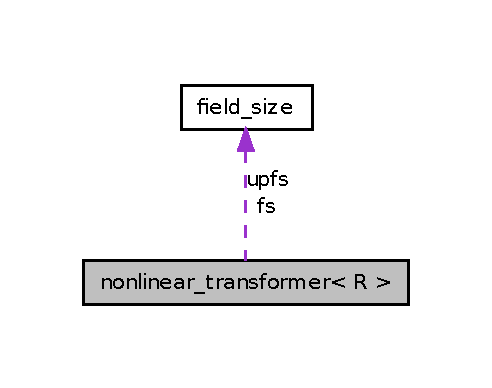
\includegraphics[width=200pt]{classnonlinear__transformer__coll__graph}
\end{center}
\end{figure}
\subsection*{Public Member Functions}
\begin{DoxyCompactItemize}
\item 
\hypertarget{classnonlinear__transformer_a5a38e3a2f6fcef5e3795f4d62ff00243}{
{\bfseries nonlinear\_\-transformer} (\hyperlink{structfield__size}{field\_\-size} \&fs\_\-, \hyperlink{structmodel__params}{model\_\-params}$<$ R $>$ \&mp\_\-)}
\label{classnonlinear__transformer_a5a38e3a2f6fcef5e3795f4d62ff00243}

\item 
\hypertarget{classnonlinear__transformer_a7f8891a31a5f12a741e044665f8bf53b}{
void {\bfseries transform} (\hyperlink{classfield}{field}$<$ R $>$ \&phi, \hyperlink{classfield}{field}$<$ R $>$ \&chi, field\_\-state final\_\-state=momentum)}
\label{classnonlinear__transformer_a7f8891a31a5f12a741e044665f8bf53b}

\end{DoxyCompactItemize}
\subsection*{Public Attributes}
\begin{DoxyCompactItemize}
\item 
\hypertarget{classnonlinear__transformer_aa6670555f08b2d91682a88b0d781c7e4}{
\hyperlink{classfield}{field}$<$ R $>$ {\bfseries phi2chi}}
\label{classnonlinear__transformer_aa6670555f08b2d91682a88b0d781c7e4}

\item 
\hypertarget{classnonlinear__transformer_a64d93bb53964634981cdb78a8b7479d7}{
\hyperlink{classfield}{field}$<$ R $>$ {\bfseries chi2phi}}
\label{classnonlinear__transformer_a64d93bb53964634981cdb78a8b7479d7}

\item 
\hypertarget{classnonlinear__transformer_a55a26245b4892699539c9f2109e4f42a}{
\hyperlink{classfield}{field}$<$ R $>$ {\bfseries phi3}}
\label{classnonlinear__transformer_a55a26245b4892699539c9f2109e4f42a}

\item 
\hypertarget{classnonlinear__transformer_aa07548a929d0aa4d78ee9f97b7f47470}{
\hyperlink{classfield}{field}$<$ R $>$ {\bfseries chi3}}
\label{classnonlinear__transformer_aa07548a929d0aa4d78ee9f97b7f47470}

\item 
\hypertarget{classnonlinear__transformer_a6ca49be67d4c8794d0d36aae697e2c14}{
\hyperlink{classfield}{field}$<$ R $>$ {\bfseries phi5}}
\label{classnonlinear__transformer_a6ca49be67d4c8794d0d36aae697e2c14}

\item 
\hypertarget{classnonlinear__transformer_a8d4009c7f7509a389e51b28c5571a40c}{
\hyperlink{classfield}{field}$<$ R $>$ {\bfseries chi5}}
\label{classnonlinear__transformer_a8d4009c7f7509a389e51b28c5571a40c}

\end{DoxyCompactItemize}
\subsection*{Protected Attributes}
\begin{DoxyCompactItemize}
\item 
\hypertarget{classnonlinear__transformer_a128ffada9074a7bdc2e3ede63ae98ef1}{
\hyperlink{structfield__size}{field\_\-size} \& {\bfseries fs}}
\label{classnonlinear__transformer_a128ffada9074a7bdc2e3ede63ae98ef1}

\item 
\hypertarget{classnonlinear__transformer_a4444a064e4080b2f76a388d4256e0a28}{
\hyperlink{structfield__size}{field\_\-size} {\bfseries upfs}}
\label{classnonlinear__transformer_a4444a064e4080b2f76a388d4256e0a28}

\item 
\hypertarget{classnonlinear__transformer_a50c4033d9364f08a083817221bbe9ac9}{
\hyperlink{structmodel__params}{model\_\-params}$<$ R $>$ \& {\bfseries mp}}
\label{classnonlinear__transformer_a50c4033d9364f08a083817221bbe9ac9}

\end{DoxyCompactItemize}
\subsubsection*{template$<$typename R$>$ class nonlinear\_\-transformer$<$ R $>$}



The documentation for this class was generated from the following files:\begin{DoxyCompactItemize}
\item 
\hyperlink{nonlinear__transformer_8hpp}{nonlinear\_\-transformer.hpp}\item 
nonlinear\_\-transformer.cpp\end{DoxyCompactItemize}

\hypertarget{classrk4}{
\section{rk4$<$ R $>$ Class Template Reference}
\label{classrk4}\index{rk4@{rk4}}
}
Inheritance diagram for rk4$<$ R $>$:\nopagebreak
\begin{figure}[H]
\begin{center}
\leavevmode
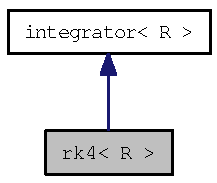
\includegraphics[width=140pt]{classrk4__inherit__graph}
\end{center}
\end{figure}
Collaboration diagram for rk4$<$ R $>$:\nopagebreak
\begin{figure}[H]
\begin{center}
\leavevmode
\includegraphics[width=220pt]{classrk4__coll__graph}
\end{center}
\end{figure}
\subsection*{Public Member Functions}
\begin{DoxyCompactItemize}
\item 
\hypertarget{classrk4_a6b6538e79bab2ccb9b65b953f8871073}{
{\bfseries rk4} (\hyperlink{structfield__size}{field\_\-size} \&fs\_\-, \hyperlink{structmodel__params}{model\_\-params}$<$ R $>$ \&mp\_\-, \hyperlink{structtime__state}{time\_\-state}$<$ R $>$ \&ts\_\-, \hyperlink{classfield}{field}$<$ R $>$ \&phi\_\-, \hyperlink{classfield}{field}$<$ R $>$ \&phidot\_\-, \hyperlink{classfield}{field}$<$ R $>$ \&chi\_\-, \hyperlink{classfield}{field}$<$ R $>$ \&chidot\_\-)}
\label{classrk4_a6b6538e79bab2ccb9b65b953f8871073}

\item 
\hypertarget{classrk4_a10c9b1ff5a625427a90f5d235c0d4aec}{
virtual void {\bfseries step} ()}
\label{classrk4_a10c9b1ff5a625427a90f5d235c0d4aec}

\item 
\hypertarget{classrk4_a1925c4efac74de9bec188b4c6c5a3b1c}{
virtual void {\bfseries initialize} ()}
\label{classrk4_a1925c4efac74de9bec188b4c6c5a3b1c}

\end{DoxyCompactItemize}
\subsection*{Protected Member Functions}
\begin{DoxyCompactItemize}
\item 
\hypertarget{classrk4_a32ca7b0812b646d626ef2581e9a7558d}{
void {\bfseries substep\_\-scale} (R fac, \hyperlink{classfield}{field}$<$ R $>$ \&phip, \hyperlink{classfield}{field}$<$ R $>$ \&chip, R ap, R adotp, R ptp, R \&an, R \&adotn, R \&ptn, R \&dan, R \&dadotn, R \&dptn, R \&avg\_\-gradient\_\-phi, R \&avg\_\-gradient\_\-chi)}
\label{classrk4_a32ca7b0812b646d626ef2581e9a7558d}

\item 
\hypertarget{classrk4_ab6588276335620de871fadf2065059b9}{
void {\bfseries substep} (R fac, \hyperlink{classfield}{field}$<$ R $>$ \&phip, \hyperlink{classfield}{field}$<$ R $>$ \&chip, \hyperlink{classfield}{field}$<$ R $>$ \&phidotp, \hyperlink{classfield}{field}$<$ R $>$ \&chidotp, \hyperlink{classfield}{field}$<$ R $>$ \&phin, \hyperlink{classfield}{field}$<$ R $>$ \&chin, \hyperlink{classfield}{field}$<$ R $>$ \&phidotn, \hyperlink{classfield}{field}$<$ R $>$ \&chidotn, R ap, R adotp, R ptp, R \&an, R \&adotn, R \&ptn, R \&avg\_\-gradient\_\-phi, R \&avg\_\-gradient\_\-chi)}
\label{classrk4_ab6588276335620de871fadf2065059b9}

\end{DoxyCompactItemize}
\subsection*{Protected Attributes}
\begin{DoxyCompactItemize}
\item 
\hypertarget{classrk4_afe0b3e6a2f96cea1ebe881ca0aef0862}{
\hyperlink{structfield__size}{field\_\-size} \& {\bfseries fs}}
\label{classrk4_afe0b3e6a2f96cea1ebe881ca0aef0862}

\item 
\hypertarget{classrk4_a9cdc6aaad4517190a829e845eab95447}{
\hyperlink{structfield__size}{field\_\-size} {\bfseries upfs}}
\label{classrk4_a9cdc6aaad4517190a829e845eab95447}

\item 
\hypertarget{classrk4_a581eef6e9ad6b101b04c93d051e4f634}{
\hyperlink{structmodel__params}{model\_\-params}$<$ R $>$ \& {\bfseries mp}}
\label{classrk4_a581eef6e9ad6b101b04c93d051e4f634}

\item 
\hypertarget{classrk4_a55651dfa97a653e008c40de715e60825}{
\hyperlink{structtime__state}{time\_\-state}$<$ R $>$ \& {\bfseries ts}}
\label{classrk4_a55651dfa97a653e008c40de715e60825}

\item 
\hypertarget{classrk4_a9760be7b78db1d69e367e2e77442e0c1}{
\hyperlink{classfield}{field}$<$ R $>$ \& {\bfseries phi}}
\label{classrk4_a9760be7b78db1d69e367e2e77442e0c1}

\item 
\hypertarget{classrk4_acb8d6d981d3f0f1a0a117493e4e51e7f}{
\hyperlink{classfield}{field}$<$ R $>$ \& {\bfseries phidot}}
\label{classrk4_acb8d6d981d3f0f1a0a117493e4e51e7f}

\item 
\hypertarget{classrk4_a8c46486589b9dcb6c58c339373e0bdf8}{
\hyperlink{classfield}{field}$<$ R $>$ \& {\bfseries chi}}
\label{classrk4_a8c46486589b9dcb6c58c339373e0bdf8}

\item 
\hypertarget{classrk4_ad3b83eb5a6571a9549b3c69b019a51f3}{
\hyperlink{classfield}{field}$<$ R $>$ \& {\bfseries chidot}}
\label{classrk4_ad3b83eb5a6571a9549b3c69b019a51f3}

\item 
\hypertarget{classrk4_a699dedb5a35ca9ba4f79c4aef5d7865d}{
\hyperlink{classfield}{field}$<$ R $>$ {\bfseries phi1}}
\label{classrk4_a699dedb5a35ca9ba4f79c4aef5d7865d}

\item 
\hypertarget{classrk4_aaf72f8162b7ed592d19cf0d9c83b6d46}{
\hyperlink{classfield}{field}$<$ R $>$ {\bfseries phidot1}}
\label{classrk4_aaf72f8162b7ed592d19cf0d9c83b6d46}

\item 
\hypertarget{classrk4_a2a4283efb5c57af1208a2cee767a4e85}{
\hyperlink{classfield}{field}$<$ R $>$ {\bfseries chi1}}
\label{classrk4_a2a4283efb5c57af1208a2cee767a4e85}

\item 
\hypertarget{classrk4_acd47b50e18dccede25777f0da1b55331}{
\hyperlink{classfield}{field}$<$ R $>$ {\bfseries chidot1}}
\label{classrk4_acd47b50e18dccede25777f0da1b55331}

\item 
\hypertarget{classrk4_a770d191019daa7bd12a0efeb9ed87217}{
\hyperlink{classfield}{field}$<$ R $>$ {\bfseries phi2}}
\label{classrk4_a770d191019daa7bd12a0efeb9ed87217}

\item 
\hypertarget{classrk4_a6fb65966932e72bfbef4244434c8d51e}{
\hyperlink{classfield}{field}$<$ R $>$ {\bfseries phidot2}}
\label{classrk4_a6fb65966932e72bfbef4244434c8d51e}

\item 
\hypertarget{classrk4_a44ba4ba2640a3e0014270c43b26427cf}{
\hyperlink{classfield}{field}$<$ R $>$ {\bfseries chi2}}
\label{classrk4_a44ba4ba2640a3e0014270c43b26427cf}

\item 
\hypertarget{classrk4_af7bbc770e6294ab619da641bf4923eb3}{
\hyperlink{classfield}{field}$<$ R $>$ {\bfseries chidot2}}
\label{classrk4_af7bbc770e6294ab619da641bf4923eb3}

\item 
\hypertarget{classrk4_a08bea04f3eee6087c6a516493eedfd88}{
\hyperlink{classfield}{field}$<$ R $>$ {\bfseries phi3}}
\label{classrk4_a08bea04f3eee6087c6a516493eedfd88}

\item 
\hypertarget{classrk4_a106dcf5d9a31129ed0af0e3df3f0d147}{
\hyperlink{classfield}{field}$<$ R $>$ {\bfseries phidot3}}
\label{classrk4_a106dcf5d9a31129ed0af0e3df3f0d147}

\item 
\hypertarget{classrk4_af5c55d0ad747dd298a2d09f017177783}{
\hyperlink{classfield}{field}$<$ R $>$ {\bfseries chi3}}
\label{classrk4_af5c55d0ad747dd298a2d09f017177783}

\item 
\hypertarget{classrk4_a9a8e3aa6dd0323757e174e087ce3f10d}{
\hyperlink{classfield}{field}$<$ R $>$ {\bfseries chidot3}}
\label{classrk4_a9a8e3aa6dd0323757e174e087ce3f10d}

\item 
\hypertarget{classrk4_a214560be9771a0fd1e1d3450685da9c5}{
\hyperlink{classnonlinear__transformer}{nonlinear\_\-transformer}$<$ R $>$ {\bfseries nlt}}
\label{classrk4_a214560be9771a0fd1e1d3450685da9c5}

\item 
\hypertarget{classrk4_a5e52ad362e80169cc3f23b1c0f3a7a4f}{
\hyperlink{classv__integrator}{v\_\-integrator}$<$ R $>$ {\bfseries vi}}
\label{classrk4_a5e52ad362e80169cc3f23b1c0f3a7a4f}

\item 
\hypertarget{classrk4_a765791d03fef48a8f9593eaca27defc8}{
R {\bfseries a1}}
\label{classrk4_a765791d03fef48a8f9593eaca27defc8}

\item 
\hypertarget{classrk4_acfeb66ce99e18d056afcaa505d3b7a96}{
R {\bfseries a2}}
\label{classrk4_acfeb66ce99e18d056afcaa505d3b7a96}

\item 
\hypertarget{classrk4_a7e382e7de3e229aa630f9db784606132}{
R {\bfseries a3}}
\label{classrk4_a7e382e7de3e229aa630f9db784606132}

\item 
\hypertarget{classrk4_a8a815689314b092fa0efd0765a3ad72e}{
R {\bfseries a4}}
\label{classrk4_a8a815689314b092fa0efd0765a3ad72e}

\item 
\hypertarget{classrk4_ae4b5442df2eaad12af507fc6b6cc39f8}{
R {\bfseries adot1}}
\label{classrk4_ae4b5442df2eaad12af507fc6b6cc39f8}

\item 
\hypertarget{classrk4_a879967a2a1270776afa585f5850c727f}{
R {\bfseries adot2}}
\label{classrk4_a879967a2a1270776afa585f5850c727f}

\item 
\hypertarget{classrk4_a350891ddc4b25427b0079ab2fdcbe4a1}{
R {\bfseries adot3}}
\label{classrk4_a350891ddc4b25427b0079ab2fdcbe4a1}

\item 
\hypertarget{classrk4_a07c2ff2eacda1d97394b3dee74229cae}{
R {\bfseries adot4}}
\label{classrk4_a07c2ff2eacda1d97394b3dee74229cae}

\item 
\hypertarget{classrk4_aed79efad1fa1ea909519e1a6014534ed}{
R {\bfseries pt1}}
\label{classrk4_aed79efad1fa1ea909519e1a6014534ed}

\item 
\hypertarget{classrk4_afe0e73a59a9fbf83b4ad4d712a6c174f}{
R {\bfseries pt2}}
\label{classrk4_afe0e73a59a9fbf83b4ad4d712a6c174f}

\item 
\hypertarget{classrk4_af6d1c9355312c55dfc0d16655c267149}{
R {\bfseries pt3}}
\label{classrk4_af6d1c9355312c55dfc0d16655c267149}

\item 
\hypertarget{classrk4_a985405ea783dcb3c49a3675c98378012}{
R {\bfseries pt4}}
\label{classrk4_a985405ea783dcb3c49a3675c98378012}

\end{DoxyCompactItemize}
\subsubsection*{template$<$typename R$>$ class rk4$<$ R $>$}



The documentation for this class was generated from the following files:\begin{DoxyCompactItemize}
\item 
\hyperlink{rk4_8hpp}{rk4.hpp}\item 
rk4.cpp\end{DoxyCompactItemize}

\hypertarget{structrs__init}{
\section{rs\_\-init$<$ R $>$ Struct Template Reference}
\label{structrs__init}\index{rs\_\-init@{rs\_\-init}}
}
Collaboration diagram for rs\_\-init$<$ R $>$:\nopagebreak
\begin{figure}[H]
\begin{center}
\leavevmode
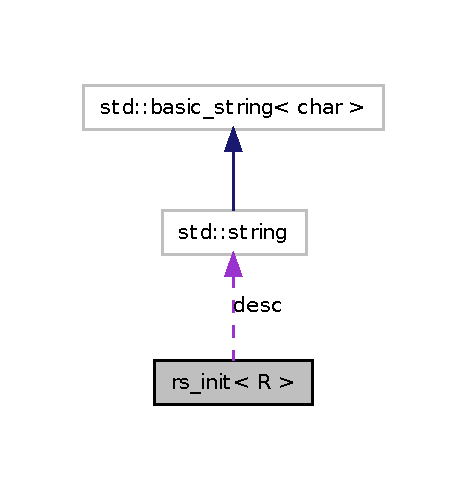
\includegraphics[width=188pt]{structrs__init__coll__graph}
\end{center}
\end{figure}
\subsection*{Public Member Functions}
\begin{DoxyCompactItemize}
\item 
\hypertarget{structrs__init_a93198ddfe0f8ffcfe2ee57df20cd78c5}{
{\bfseries rs\_\-init} (R m, R B, R s, R r, R A, const std::string \&d)}
\label{structrs__init_a93198ddfe0f8ffcfe2ee57df20cd78c5}

\item 
\hypertarget{structrs__init_aaca9f6a2e74df7095086c719d84756b3}{
bool {\bfseries operator$<$} (const \hyperlink{structrs__init}{rs\_\-init} \&rs) const }
\label{structrs__init_aaca9f6a2e74df7095086c719d84756b3}

\end{DoxyCompactItemize}
\subsection*{Public Attributes}
\begin{DoxyCompactItemize}
\item 
\hypertarget{structrs__init_a8fa698ef5e1f5151d0393c836d84f780}{
R {\bfseries mag}}
\label{structrs__init_a8fa698ef5e1f5151d0393c836d84f780}

\item 
\hypertarget{structrs__init_a0a8127cb70006a9d1a41d4ebf17b9cb2}{
R {\bfseries rescale\_\-B}}
\label{structrs__init_a0a8127cb70006a9d1a41d4ebf17b9cb2}

\item 
\hypertarget{structrs__init_a32db36edb844b37147b363e8d53b68b5}{
R {\bfseries rescale\_\-s}}
\label{structrs__init_a32db36edb844b37147b363e8d53b68b5}

\item 
\hypertarget{structrs__init_a33b5a3f878b4f7b9284a7537895a82b8}{
R {\bfseries rescale\_\-r}}
\label{structrs__init_a33b5a3f878b4f7b9284a7537895a82b8}

\item 
\hypertarget{structrs__init_aa6fbf7fda7d4907c3e6af6153a2ef4d1}{
R {\bfseries rescale\_\-A}}
\label{structrs__init_aa6fbf7fda7d4907c3e6af6153a2ef4d1}

\item 
\hypertarget{structrs__init_a649b9690f64e93b8c5098a5d53235b70}{
std::string {\bfseries desc}}
\label{structrs__init_a649b9690f64e93b8c5098a5d53235b70}

\end{DoxyCompactItemize}
\subsubsection*{template$<$typename R$>$ struct rs\_\-init$<$ R $>$}



The documentation for this struct was generated from the following file:\begin{DoxyCompactItemize}
\item 
\hyperlink{model__params_8hpp}{model\_\-params.hpp}\end{DoxyCompactItemize}

\hypertarget{classslice__output__manager}{
\section{slice\_\-output\_\-manager$<$ R $>$ Class Template Reference}
\label{classslice__output__manager}\index{slice\_\-output\_\-manager@{slice\_\-output\_\-manager}}
}


Collaboration diagram for slice\_\-output\_\-manager$<$ R $>$:
\nopagebreak
\begin{figure}[H]
\begin{center}
\leavevmode
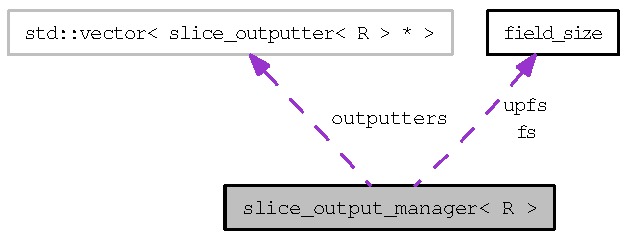
\includegraphics[width=372pt]{classslice__output__manager__coll__graph}
\end{center}
\end{figure}
\subsection*{Public Types}
\begin{DoxyCompactItemize}
\item 
\hypertarget{classslice__output__manager_a52e08ac6e50f8f93dd50412350c03b1a}{
typedef \hyperlink{classslice__outputter}{slice\_\-outputter}$<$ R $>$::var\_\-func {\bfseries var\_\-func}}
\label{classslice__output__manager_a52e08ac6e50f8f93dd50412350c03b1a}

\end{DoxyCompactItemize}
\subsection*{Public Member Functions}
\begin{DoxyCompactItemize}
\item 
\hypertarget{classslice__output__manager_abe4f0eeea3e5288c6c168de759dd6096}{
{\bfseries slice\_\-output\_\-manager} (\hyperlink{structfield__size}{field\_\-size} \&fs\_\-, \hyperlink{structmodel__params}{model\_\-params}$<$ R $>$ \&mp\_\-, \hyperlink{structtime__state}{time\_\-state}$<$ R $>$ \&ts\_\-, \hyperlink{classfield}{field}$<$ R $>$ \&phi\_\-, \hyperlink{classfield}{field}$<$ R $>$ \&chi\_\-, \hyperlink{classfield}{field}$<$ R $>$ \&phidot\_\-, \hyperlink{classfield}{field}$<$ R $>$ \&chidot\_\-, \hyperlink{classgrad__computer}{grad\_\-computer}$<$ R $>$ \&gc\_\-, \hyperlink{classgpot__computer}{gpot\_\-computer}$<$ R $>$ \&gpotc\_\-, int slicedim\_\-=3, int slicelength\_\-=0, int sliceskip\_\-=1, bool sliceaverage\_\-=true, bool sliceflt\_\-=true)}
\label{classslice__output__manager_abe4f0eeea3e5288c6c168de759dd6096}

\item 
\hypertarget{classslice__output__manager_a0864d241251993f377fe46cb63b1cc3b}{
void {\bfseries add\_\-outputter} (std::string varname, var\_\-func vf)}
\label{classslice__output__manager_a0864d241251993f377fe46cb63b1cc3b}

\item 
\hypertarget{classslice__output__manager_a5ee2088a87d16e709caf41860063d4ab}{
void {\bfseries output} ()}
\label{classslice__output__manager_a5ee2088a87d16e709caf41860063d4ab}

\end{DoxyCompactItemize}
\subsection*{Protected Attributes}
\begin{DoxyCompactItemize}
\item 
\hypertarget{classslice__output__manager_a6e478c6b654b96779a5210246e38966b}{
\hyperlink{structfield__size}{field\_\-size} \& {\bfseries fs}}
\label{classslice__output__manager_a6e478c6b654b96779a5210246e38966b}

\item 
\hypertarget{classslice__output__manager_a5013ff50d2d91fb02b40641ee76565e7}{
\hyperlink{structfield__size}{field\_\-size} {\bfseries upfs}}
\label{classslice__output__manager_a5013ff50d2d91fb02b40641ee76565e7}

\item 
\hypertarget{classslice__output__manager_aedfefca04cda214b143f51ff5e4d0abc}{
\hyperlink{structmodel__params}{model\_\-params}$<$ R $>$ \& {\bfseries mp}}
\label{classslice__output__manager_aedfefca04cda214b143f51ff5e4d0abc}

\item 
\hypertarget{classslice__output__manager_a2e319ab07b2f053b52887c53029b4d56}{
\hyperlink{structtime__state}{time\_\-state}$<$ R $>$ \& {\bfseries ts}}
\label{classslice__output__manager_a2e319ab07b2f053b52887c53029b4d56}

\item 
\hypertarget{classslice__output__manager_acc6e7ed40233dd325ee649646848aa1c}{
\hyperlink{classfield}{field}$<$ R $>$ \& {\bfseries phi}}
\label{classslice__output__manager_acc6e7ed40233dd325ee649646848aa1c}

\item 
\hypertarget{classslice__output__manager_a32c5db379879919d9622301199db7a7b}{
\hyperlink{classfield}{field}$<$ R $>$ \& {\bfseries chi}}
\label{classslice__output__manager_a32c5db379879919d9622301199db7a7b}

\item 
\hypertarget{classslice__output__manager_a13e320a0a520f6b53df60e556332d4cc}{
\hyperlink{classfield}{field}$<$ R $>$ \& {\bfseries phidot}}
\label{classslice__output__manager_a13e320a0a520f6b53df60e556332d4cc}

\item 
\hypertarget{classslice__output__manager_a1bd87399bedf30886d9f412e25f2ad24}{
\hyperlink{classfield}{field}$<$ R $>$ \& {\bfseries chidot}}
\label{classslice__output__manager_a1bd87399bedf30886d9f412e25f2ad24}

\item 
\hypertarget{classslice__output__manager_aef9191da41665323b7b552c1cac39025}{
\hyperlink{classgrad__computer}{grad\_\-computer}$<$ R $>$ \& {\bfseries gc}}
\label{classslice__output__manager_aef9191da41665323b7b552c1cac39025}

\item 
\hypertarget{classslice__output__manager_a4c23fefda63c2c5cb29f73d73374913e}{
\hyperlink{classgpot__computer}{gpot\_\-computer}$<$ R $>$ \& {\bfseries gpotc}}
\label{classslice__output__manager_a4c23fefda63c2c5cb29f73d73374913e}

\item 
\hypertarget{classslice__output__manager_ab53afdf80adec6a9a06869a11a9c6394}{
int {\bfseries slicedim}}
\label{classslice__output__manager_ab53afdf80adec6a9a06869a11a9c6394}

\item 
\hypertarget{classslice__output__manager_ab16957b5fabbc0068c33ac4bf431085d}{
int {\bfseries slicelength}}
\label{classslice__output__manager_ab16957b5fabbc0068c33ac4bf431085d}

\item 
\hypertarget{classslice__output__manager_aa01a399598c39945b501b1ff9d2a0829}{
int {\bfseries sliceskip}}
\label{classslice__output__manager_aa01a399598c39945b501b1ff9d2a0829}

\item 
\hypertarget{classslice__output__manager_afdd5365b8dcbf9a1e948c476cd28ecc2}{
bool {\bfseries sliceaverage}}
\label{classslice__output__manager_afdd5365b8dcbf9a1e948c476cd28ecc2}

\item 
\hypertarget{classslice__output__manager_ad286ed8d06a07e2c98ae506718165162}{
bool {\bfseries sliceflt}}
\label{classslice__output__manager_ad286ed8d06a07e2c98ae506718165162}

\item 
\hypertarget{classslice__output__manager_a1fe93dc74b0853ed83416439e286d898}{
int {\bfseries bin\_\-idx}}
\label{classslice__output__manager_a1fe93dc74b0853ed83416439e286d898}

\item 
\hypertarget{classslice__output__manager_a3c7aaa9dec8709ad63c587816808d77b}{
std::vector$<$ \hyperlink{classslice__outputter}{slice\_\-outputter}$<$ R $>$ $\ast$ $>$ {\bfseries outputters}}
\label{classslice__output__manager_a3c7aaa9dec8709ad63c587816808d77b}

\end{DoxyCompactItemize}
\subsubsection*{template$<$typename R$>$ class slice\_\-output\_\-manager$<$ R $>$}



The documentation for this class was generated from the following files:\begin{DoxyCompactItemize}
\item 
\hyperlink{slice__output__manager_8hpp}{slice\_\-output\_\-manager.hpp}\item 
slice\_\-output\_\-manager.cpp\end{DoxyCompactItemize}

\hypertarget{classslice__outputter}{
\section{slice\_\-outputter$<$ R $>$ Class Template Reference}
\label{classslice__outputter}\index{slice\_\-outputter@{slice\_\-outputter}}
}
Collaboration diagram for slice\_\-outputter$<$ R $>$:\nopagebreak
\begin{figure}[H]
\begin{center}
\leavevmode
\includegraphics[width=372pt]{classslice__outputter__coll__graph}
\end{center}
\end{figure}
\subsection*{Public Types}
\begin{DoxyCompactItemize}
\item 
\hypertarget{classslice__outputter_a0917a3b6bc70da35b0b2344342d9ab87}{
typedef R($\ast$ {\bfseries var\_\-func} )(\hyperlink{structfield__size}{field\_\-size} \&fs, \hyperlink{structmodel__params}{model\_\-params}$<$ R $>$ \&mp, \hyperlink{structtime__state}{time\_\-state}$<$ R $>$ \&ts, R phi, R chi, R phidot, R chidot, R phigradx, R chigradx, R phigrady, R chigrady, R phigradz, R chigradz, R gpot)}
\label{classslice__outputter_a0917a3b6bc70da35b0b2344342d9ab87}

\end{DoxyCompactItemize}
\subsection*{Public Member Functions}
\begin{DoxyCompactItemize}
\item 
\hypertarget{classslice__outputter_a6ea080464c3e9dbe3d85414335e37e84}{
{\bfseries slice\_\-outputter} (\hyperlink{structfield__size}{field\_\-size} \&fs\_\-, \hyperlink{structmodel__params}{model\_\-params}$<$ R $>$ \&mp\_\-, \hyperlink{structtime__state}{time\_\-state}$<$ R $>$ \&ts\_\-, int slicelength\_\-, std::string varname\_\-, var\_\-func vf\_\-)}
\label{classslice__outputter_a6ea080464c3e9dbe3d85414335e37e84}

\item 
\hypertarget{classslice__outputter_a4a9c77e60f5bc6b7f83e2063e5d6e334}{
void {\bfseries begin} (int bin\_\-idx)}
\label{classslice__outputter_a4a9c77e60f5bc6b7f83e2063e5d6e334}

\item 
\hypertarget{classslice__outputter_aa9fe19a69c103855544940ad2b32c01a}{
void {\bfseries flush} ()}
\label{classslice__outputter_aa9fe19a69c103855544940ad2b32c01a}

\item 
\hypertarget{classslice__outputter_a5d9762160a8e538880df5ff44b84f3c6}{
void {\bfseries advance} ()}
\label{classslice__outputter_a5d9762160a8e538880df5ff44b84f3c6}

\item 
\hypertarget{classslice__outputter_a8ec331e66afb581d8d70bd5630e7f857}{
void {\bfseries accumulate} (R phi, R chi, R phidot, R chidot, R phigradx, R chigradx, R phigrady, R chigrady, R phigradz, R chigradz, R gpot)}
\label{classslice__outputter_a8ec331e66afb581d8d70bd5630e7f857}

\end{DoxyCompactItemize}
\subsection*{Protected Attributes}
\begin{DoxyCompactItemize}
\item 
\hypertarget{classslice__outputter_a957a690d81a02f59d57327de464738f4}{
\hyperlink{structfield__size}{field\_\-size} \& {\bfseries fs}}
\label{classslice__outputter_a957a690d81a02f59d57327de464738f4}

\item 
\hypertarget{classslice__outputter_ad86ae98d01e3cfa301f070df0c34e9da}{
\hyperlink{structmodel__params}{model\_\-params}$<$ R $>$ \& {\bfseries mp}}
\label{classslice__outputter_ad86ae98d01e3cfa301f070df0c34e9da}

\item 
\hypertarget{classslice__outputter_a83c1dda3296ff12af9729fbc2210205f}{
\hyperlink{structtime__state}{time\_\-state}$<$ R $>$ \& {\bfseries ts}}
\label{classslice__outputter_a83c1dda3296ff12af9729fbc2210205f}

\item 
\hypertarget{classslice__outputter_adf3e27259b0f4318b4a9a00106df6d96}{
int {\bfseries slicelength}}
\label{classslice__outputter_adf3e27259b0f4318b4a9a00106df6d96}

\item 
\hypertarget{classslice__outputter_a4a70ac08cb89e853a490ece136cd5010}{
std::string {\bfseries varname}}
\label{classslice__outputter_a4a70ac08cb89e853a490ece136cd5010}

\item 
\hypertarget{classslice__outputter_a0b706216df5e16b436668b0d3bc6a16b}{
var\_\-func {\bfseries vf}}
\label{classslice__outputter_a0b706216df5e16b436668b0d3bc6a16b}

\item 
\hypertarget{classslice__outputter_a90523789057b3046d3f46dde7bfebd03}{
R $\ast$ {\bfseries buffer}}
\label{classslice__outputter_a90523789057b3046d3f46dde7bfebd03}

\item 
\hypertarget{classslice__outputter_ab6e8e5c34ae2e3e89cd376543eb0a937}{
float $\ast$ {\bfseries bufferf}}
\label{classslice__outputter_ab6e8e5c34ae2e3e89cd376543eb0a937}

\item 
\hypertarget{classslice__outputter_a6af61ed3f846ca2e1bedc34db4bfb30b}{
std::ofstream {\bfseries of}}
\label{classslice__outputter_a6af61ed3f846ca2e1bedc34db4bfb30b}

\item 
\hypertarget{classslice__outputter_ab54a5b462f4ca3f3ef4c433177b2ef42}{
int {\bfseries cp}}
\label{classslice__outputter_ab54a5b462f4ca3f3ef4c433177b2ef42}

\item 
\hypertarget{classslice__outputter_a847f8e4abb0bcf1f9ee5ee3269949c6b}{
int {\bfseries cn}}
\label{classslice__outputter_a847f8e4abb0bcf1f9ee5ee3269949c6b}

\end{DoxyCompactItemize}
\subsubsection*{template$<$typename R$>$ class slice\_\-outputter$<$ R $>$}



The documentation for this class was generated from the following files:\begin{DoxyCompactItemize}
\item 
\hyperlink{slice__outputter_8hpp}{slice\_\-outputter.hpp}\item 
slice\_\-outputter.cpp\end{DoxyCompactItemize}

\hypertarget{classspectra__outputter}{
\section{spectra\_\-outputter$<$ R $>$ Class Template Reference}
\label{classspectra__outputter}\index{spectra\_\-outputter@{spectra\_\-outputter}}
}


Collaboration diagram for spectra\_\-outputter$<$ R $>$:
\nopagebreak
\begin{figure}[H]
\begin{center}
\leavevmode
\includegraphics[width=292pt]{classspectra__outputter__coll__graph}
\end{center}
\end{figure}
\subsection*{Public Member Functions}
\begin{DoxyCompactItemize}
\item 
\hypertarget{classspectra__outputter_aa65c78886ac0787088268f9991bcf5dd}{
{\bfseries spectra\_\-outputter} (\hyperlink{structfield__size}{field\_\-size} \&fs\_\-, \hyperlink{structmodel__params}{model\_\-params}$<$ R $>$ \&mp\_\-, \hyperlink{structtime__state}{time\_\-state}$<$ R $>$ \&ts\_\-, \hyperlink{classfield}{field}$<$ R $>$ \&phi\_\-, \hyperlink{classfield}{field}$<$ R $>$ \&chi\_\-)}
\label{classspectra__outputter_aa65c78886ac0787088268f9991bcf5dd}

\item 
\hypertarget{classspectra__outputter_ad5d72a350a351d5b062c3778b32e66b8}{
void {\bfseries output} ()}
\label{classspectra__outputter_ad5d72a350a351d5b062c3778b32e66b8}

\end{DoxyCompactItemize}
\subsection*{Protected Attributes}
\begin{DoxyCompactItemize}
\item 
\hypertarget{classspectra__outputter_a12d3d2c464b0b5c0af90f7be207edef0}{
\hyperlink{structfield__size}{field\_\-size} \& {\bfseries fs}}
\label{classspectra__outputter_a12d3d2c464b0b5c0af90f7be207edef0}

\item 
\hypertarget{classspectra__outputter_a41ab1e21ea2981a3499a169f6ba6d5d5}{
\hyperlink{structmodel__params}{model\_\-params}$<$ R $>$ \& {\bfseries mp}}
\label{classspectra__outputter_a41ab1e21ea2981a3499a169f6ba6d5d5}

\item 
\hypertarget{classspectra__outputter_afd83755cd068d131af002457a14e4ed8}{
\hyperlink{structtime__state}{time\_\-state}$<$ R $>$ \& {\bfseries ts}}
\label{classspectra__outputter_afd83755cd068d131af002457a14e4ed8}

\item 
\hypertarget{classspectra__outputter_a163e75801ba0b44efc9e939bfab452ce}{
\hyperlink{classfield}{field}$<$ R $>$ \& {\bfseries phi}}
\label{classspectra__outputter_a163e75801ba0b44efc9e939bfab452ce}

\item 
\hypertarget{classspectra__outputter_a8a3db4d22612373e6f77401d28bdbb0c}{
\hyperlink{classfield}{field}$<$ R $>$ \& {\bfseries chi}}
\label{classspectra__outputter_a8a3db4d22612373e6f77401d28bdbb0c}

\item 
\hypertarget{classspectra__outputter_a9c196104251f992e943b6a1ae932492c}{
std::ofstream {\bfseries of}}
\label{classspectra__outputter_a9c196104251f992e943b6a1ae932492c}

\item 
\hypertarget{classspectra__outputter_a900de002e847c9fcc6ec119ea575639e}{
R $\ast$ {\bfseries phi\_\-total}}
\label{classspectra__outputter_a900de002e847c9fcc6ec119ea575639e}

\item 
\hypertarget{classspectra__outputter_adcec5f21a66ef3398e87026c1c1d69ff}{
R $\ast$ {\bfseries chi\_\-total}}
\label{classspectra__outputter_adcec5f21a66ef3398e87026c1c1d69ff}

\item 
\hypertarget{classspectra__outputter_a68b1921f43357bb22184d01c77f5f66c}{
int $\ast$ {\bfseries counts}}
\label{classspectra__outputter_a68b1921f43357bb22184d01c77f5f66c}

\end{DoxyCompactItemize}
\subsubsection*{template$<$typename R$>$ class spectra\_\-outputter$<$ R $>$}



The documentation for this class was generated from the following files:\begin{DoxyCompactItemize}
\item 
\hyperlink{spectra__outputter_8hpp}{spectra\_\-outputter.hpp}\item 
spectra\_\-outputter.cpp\end{DoxyCompactItemize}

\hypertarget{classstats__outputter}{
\section{stats\_\-outputter$<$ R $>$ Class Template Reference}
\label{classstats__outputter}\index{stats\_\-outputter@{stats\_\-outputter}}
}


Collaboration diagram for stats\_\-outputter$<$ R $>$:
\nopagebreak
\begin{figure}[H]
\begin{center}
\leavevmode
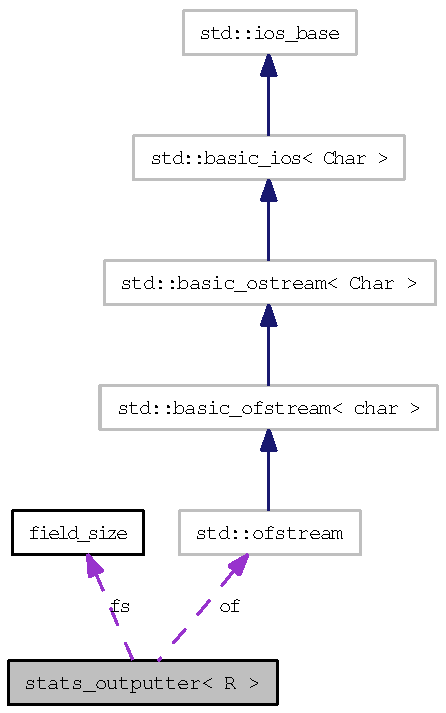
\includegraphics[width=286pt]{classstats__outputter__coll__graph}
\end{center}
\end{figure}
\subsection*{Public Member Functions}
\begin{DoxyCompactItemize}
\item 
\hypertarget{classstats__outputter_a12a507e68b035ff1d5bd588baf9e0a31}{
{\bfseries stats\_\-outputter} (\hyperlink{structfield__size}{field\_\-size} \&fs\_\-, \hyperlink{structmodel__params}{model\_\-params}$<$ R $>$ \&mp\_\-, \hyperlink{structtime__state}{time\_\-state}$<$ R $>$ \&ts\_\-, \hyperlink{classfield}{field}$<$ R $>$ \&phi\_\-, \hyperlink{classfield}{field}$<$ R $>$ \&chi\_\-, \hyperlink{classfield}{field}$<$ R $>$ \&phidot\_\-, \hyperlink{classfield}{field}$<$ R $>$ \&chidot\_\-)}
\label{classstats__outputter_a12a507e68b035ff1d5bd588baf9e0a31}

\item 
\hypertarget{classstats__outputter_aaeccf7473d48bec8a138e30f93f9fb9a}{
void {\bfseries output} ()}
\label{classstats__outputter_aaeccf7473d48bec8a138e30f93f9fb9a}

\end{DoxyCompactItemize}
\subsection*{Protected Member Functions}
\begin{DoxyCompactItemize}
\item 
\hypertarget{classstats__outputter_af586161d6085407cffd6ffd35f674ad8}{
void {\bfseries compute} (\hyperlink{classfield}{field}$<$ R $>$ \&fld1, \hyperlink{classfield}{field}$<$ R $>$ \&fld2, R \&fld1\_\-mean, R \&fld2\_\-mean, R \&fld1\_\-var, R \&fld2\_\-var)}
\label{classstats__outputter_af586161d6085407cffd6ffd35f674ad8}

\item 
\hypertarget{classstats__outputter_a01cb22821bb0f8fb9179c6c94260955d}{
void {\bfseries compute\_\-cov} (\hyperlink{classfield}{field}$<$ R $>$ \&fld, \hyperlink{classfield}{field}$<$ R $>$ \&flddot, R \&fld\_\-flddot\_\-cov)}
\label{classstats__outputter_a01cb22821bb0f8fb9179c6c94260955d}

\end{DoxyCompactItemize}
\subsection*{Protected Attributes}
\begin{DoxyCompactItemize}
\item 
\hypertarget{classstats__outputter_af1df1f462b7fa0b4ddf88ba3a610a5ad}{
\hyperlink{structfield__size}{field\_\-size} \& {\bfseries fs}}
\label{classstats__outputter_af1df1f462b7fa0b4ddf88ba3a610a5ad}

\item 
\hypertarget{classstats__outputter_a57040b1bf054e48394617dfb264c14d6}{
\hyperlink{structmodel__params}{model\_\-params}$<$ R $>$ \& {\bfseries mp}}
\label{classstats__outputter_a57040b1bf054e48394617dfb264c14d6}

\item 
\hypertarget{classstats__outputter_a0521e1c35bb5acadb4ce78c6b5636122}{
\hyperlink{structtime__state}{time\_\-state}$<$ R $>$ \& {\bfseries ts}}
\label{classstats__outputter_a0521e1c35bb5acadb4ce78c6b5636122}

\item 
\hypertarget{classstats__outputter_a0f99351a3034982104841cb09e7564da}{
\hyperlink{classfield}{field}$<$ R $>$ \& {\bfseries phi}}
\label{classstats__outputter_a0f99351a3034982104841cb09e7564da}

\item 
\hypertarget{classstats__outputter_a682704aa2c6cc2f8be5365bc5feabafe}{
\hyperlink{classfield}{field}$<$ R $>$ \& {\bfseries chi}}
\label{classstats__outputter_a682704aa2c6cc2f8be5365bc5feabafe}

\item 
\hypertarget{classstats__outputter_aa0cbe6f9d6e3dadba3e8dc7bd0714ea4}{
\hyperlink{classfield}{field}$<$ R $>$ \& {\bfseries phidot}}
\label{classstats__outputter_aa0cbe6f9d6e3dadba3e8dc7bd0714ea4}

\item 
\hypertarget{classstats__outputter_a6f01b31c2ba0872a70cbd7b1734417e4}{
\hyperlink{classfield}{field}$<$ R $>$ \& {\bfseries chidot}}
\label{classstats__outputter_a6f01b31c2ba0872a70cbd7b1734417e4}

\item 
\hypertarget{classstats__outputter_a918c79e8ec6dbcffee8d10ac5a79db41}{
std::ofstream {\bfseries of}}
\label{classstats__outputter_a918c79e8ec6dbcffee8d10ac5a79db41}

\end{DoxyCompactItemize}
\subsubsection*{template$<$typename R$>$ class stats\_\-outputter$<$ R $>$}



The documentation for this class was generated from the following files:\begin{DoxyCompactItemize}
\item 
\hyperlink{stats__outputter_8hpp}{stats\_\-outputter.hpp}\item 
stats\_\-outputter.cpp\end{DoxyCompactItemize}

\hypertarget{structtime__state}{
\section{time\_\-state$<$ R $>$ Struct Template Reference}
\label{structtime__state}\index{time\_\-state@{time\_\-state}}
}


Collaboration diagram for time\_\-state$<$ R $>$:
\nopagebreak
\begin{figure}[H]
\begin{center}
\leavevmode
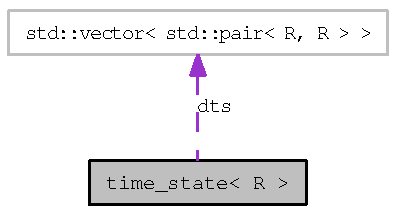
\includegraphics[width=262pt]{structtime__state__coll__graph}
\end{center}
\end{figure}
\subsection*{Public Member Functions}
\begin{DoxyCompactItemize}
\item 
\hypertarget{structtime__state_a70140623d9dde0d02302635b0848574a}{
void {\bfseries advance} ()}
\label{structtime__state_a70140623d9dde0d02302635b0848574a}

\item 
\hypertarget{structtime__state_afa54e03a4641e66c4150115137cbef65}{
void {\bfseries add\_\-dt} (R start\_\-time, R dt\_\-)}
\label{structtime__state_afa54e03a4641e66c4150115137cbef65}

\item 
\hypertarget{structtime__state_a96443b1413e21b8a8f0a4bf685d177ac}{
void {\bfseries finalize\_\-dts} ()}
\label{structtime__state_a96443b1413e21b8a8f0a4bf685d177ac}

\item 
\hypertarget{structtime__state_aeed3730c2e20e14d603781aef83f0f7e}{
void {\bfseries dt\_\-summary} (std::ostream \&os)}
\label{structtime__state_aeed3730c2e20e14d603781aef83f0f7e}

\end{DoxyCompactItemize}
\subsection*{Static Public Member Functions}
\begin{DoxyCompactItemize}
\item 
\hypertarget{structtime__state_a4b0e72b80ea35008c7022bcca39402bd}{
static R {\bfseries default\_\-dt} ()}
\label{structtime__state_a4b0e72b80ea35008c7022bcca39402bd}

\end{DoxyCompactItemize}
\subsection*{Public Attributes}
\begin{DoxyCompactItemize}
\item 
\hypertarget{structtime__state_abe9f5681bd175cf2c95846cd9242714f}{
R {\bfseries t}}
\label{structtime__state_abe9f5681bd175cf2c95846cd9242714f}

\item 
\hypertarget{structtime__state_aaa3077dc17a2e26b3df614c4731ec79e}{
R {\bfseries physical\_\-time}}
\label{structtime__state_aaa3077dc17a2e26b3df614c4731ec79e}

\item 
\hypertarget{structtime__state_afc42049df8fd72572900865bcd94d482}{
R {\bfseries a}}
\label{structtime__state_afc42049df8fd72572900865bcd94d482}

\item 
\hypertarget{structtime__state_ab97eafb749b43fae8f4f14b14f48369c}{
R {\bfseries adot}}
\label{structtime__state_ab97eafb749b43fae8f4f14b14f48369c}

\item 
\hypertarget{structtime__state_a67f019bfc07228a17c6458a2ab378668}{
R {\bfseries addot}}
\label{structtime__state_a67f019bfc07228a17c6458a2ab378668}

\item 
\hypertarget{structtime__state_a218510dd06e5bb674159c65944302034}{
R {\bfseries dt}}
\label{structtime__state_a218510dd06e5bb674159c65944302034}

\end{DoxyCompactItemize}
\subsection*{Protected Attributes}
\begin{DoxyCompactItemize}
\item 
\hypertarget{structtime__state_af2d38ab9dcf80b81c5ee07a259415a41}{
\hyperlink{structkeyed__value}{keyed\_\-value}$<$ R, R $>$ {\bfseries dtm}}
\label{structtime__state_af2d38ab9dcf80b81c5ee07a259415a41}

\end{DoxyCompactItemize}
\subsubsection*{template$<$typename R$>$ struct time\_\-state$<$ R $>$}



The documentation for this struct was generated from the following file:\begin{DoxyCompactItemize}
\item 
\hyperlink{time__state_8hpp}{time\_\-state.hpp}\end{DoxyCompactItemize}

\hypertarget{classtwoptcorr__outputter}{
\section{twoptcorr\_\-outputter$<$ R $>$ Class Template Reference}
\label{classtwoptcorr__outputter}\index{twoptcorr\_\-outputter@{twoptcorr\_\-outputter}}
}
Collaboration diagram for twoptcorr\_\-outputter$<$ R $>$:\nopagebreak
\begin{figure}[H]
\begin{center}
\leavevmode
\includegraphics[width=259pt]{classtwoptcorr__outputter__coll__graph}
\end{center}
\end{figure}
\subsection*{Public Member Functions}
\begin{DoxyCompactItemize}
\item 
\hypertarget{classtwoptcorr__outputter_aa12c83b128baced2f5bbd21e5399de5d}{
{\bfseries twoptcorr\_\-outputter} (\hyperlink{structfield__size}{field\_\-size} \&fs\_\-, \hyperlink{structmodel__params}{model\_\-params}$<$ R $>$ \&mp\_\-, \hyperlink{structtime__state}{time\_\-state}$<$ R $>$ \&ts\_\-, \hyperlink{classfield}{field}$<$ R $>$ \&phi\_\-, \hyperlink{classfield}{field}$<$ R $>$ \&chi\_\-)}
\label{classtwoptcorr__outputter_aa12c83b128baced2f5bbd21e5399de5d}

\item 
\hypertarget{classtwoptcorr__outputter_acd3fabba4d534ed9f028603562bc533f}{
void {\bfseries output} ()}
\label{classtwoptcorr__outputter_acd3fabba4d534ed9f028603562bc533f}

\end{DoxyCompactItemize}
\subsection*{Protected Attributes}
\begin{DoxyCompactItemize}
\item 
\hypertarget{classtwoptcorr__outputter_acb197f61e99dbc1e8885ff8fce520a19}{
\hyperlink{structfield__size}{field\_\-size} \& {\bfseries fs}}
\label{classtwoptcorr__outputter_acb197f61e99dbc1e8885ff8fce520a19}

\item 
\hypertarget{classtwoptcorr__outputter_a47106f6a427ebfaf85d52a57585e3e13}{
\hyperlink{structfield__size}{field\_\-size} {\bfseries upfs}}
\label{classtwoptcorr__outputter_a47106f6a427ebfaf85d52a57585e3e13}

\item 
\hypertarget{classtwoptcorr__outputter_a5bfd6082ecef6655a4cfa18bf4a41968}{
\hyperlink{structmodel__params}{model\_\-params}$<$ R $>$ \& {\bfseries mp}}
\label{classtwoptcorr__outputter_a5bfd6082ecef6655a4cfa18bf4a41968}

\item 
\hypertarget{classtwoptcorr__outputter_ae20d5ea680d9cc35faabef920dda3a45}{
\hyperlink{structtime__state}{time\_\-state}$<$ R $>$ \& {\bfseries ts}}
\label{classtwoptcorr__outputter_ae20d5ea680d9cc35faabef920dda3a45}

\item 
\hypertarget{classtwoptcorr__outputter_afd171353d8d61abced1e9f6f9b8342b1}{
\hyperlink{classfield}{field}$<$ R $>$ \& {\bfseries phi}}
\label{classtwoptcorr__outputter_afd171353d8d61abced1e9f6f9b8342b1}

\item 
\hypertarget{classtwoptcorr__outputter_af7115da4f012c1d7b93ce0d2ec8be542}{
\hyperlink{classfield}{field}$<$ R $>$ \& {\bfseries chi}}
\label{classtwoptcorr__outputter_af7115da4f012c1d7b93ce0d2ec8be542}

\item 
\hypertarget{classtwoptcorr__outputter_a32d7013b9ce9df4e7a6e2eaec2233f16}{
std::ofstream {\bfseries of}}
\label{classtwoptcorr__outputter_a32d7013b9ce9df4e7a6e2eaec2233f16}

\item 
\hypertarget{classtwoptcorr__outputter_a33d368aa0b8a620be4337201264fc1dc}{
R $\ast$ {\bfseries phi\_\-total}}
\label{classtwoptcorr__outputter_a33d368aa0b8a620be4337201264fc1dc}

\item 
\hypertarget{classtwoptcorr__outputter_a66a0e2aa1fa8c7b5e38e9bf4abadeec8}{
R $\ast$ {\bfseries chi\_\-total}}
\label{classtwoptcorr__outputter_a66a0e2aa1fa8c7b5e38e9bf4abadeec8}

\item 
\hypertarget{classtwoptcorr__outputter_af7480fc82800941d6411a96d1bc5541b}{
int $\ast$ {\bfseries counts}}
\label{classtwoptcorr__outputter_af7480fc82800941d6411a96d1bc5541b}

\item 
\hypertarget{classtwoptcorr__outputter_a94311fae5d6a70fe4161b9f517175af9}{
int {\bfseries dmax}}
\label{classtwoptcorr__outputter_a94311fae5d6a70fe4161b9f517175af9}

\item 
\hypertarget{classtwoptcorr__outputter_aff7c05700048aed218b0eb8e5a45ea1e}{
\hyperlink{classfield}{field}$<$ R $>$ {\bfseries corr}}
\label{classtwoptcorr__outputter_aff7c05700048aed218b0eb8e5a45ea1e}

\end{DoxyCompactItemize}
\subsubsection*{template$<$typename R$>$ class twoptcorr\_\-outputter$<$ R $>$}



The documentation for this class was generated from the following files:\begin{DoxyCompactItemize}
\item 
\hyperlink{twoptcorr__outputter_8hpp}{twoptcorr\_\-outputter.hpp}\item 
twoptcorr\_\-outputter.cpp\end{DoxyCompactItemize}

\hypertarget{classv__integrator}{
\section{v\_\-integrator$<$ R $>$ Class Template Reference}
\label{classv__integrator}\index{v\_\-integrator@{v\_\-integrator}}
}


Collaboration diagram for v\_\-integrator$<$ R $>$:
\nopagebreak
\begin{figure}[H]
\begin{center}
\leavevmode
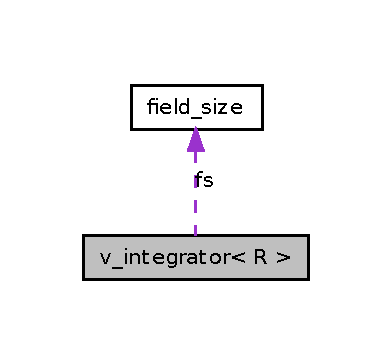
\includegraphics[width=188pt]{classv__integrator__coll__graph}
\end{center}
\end{figure}
\subsection*{Public Member Functions}
\begin{DoxyCompactItemize}
\item 
\hypertarget{classv__integrator_a2f408bba9ba58a93d1528b0a24550e4b}{
{\bfseries v\_\-integrator} (\hyperlink{structfield__size}{field\_\-size} \&fs\_\-, \hyperlink{structmodel__params}{model\_\-params}$<$ R $>$ \&mp\_\-)}
\label{classv__integrator_a2f408bba9ba58a93d1528b0a24550e4b}

\item 
\hypertarget{classv__integrator_a2540dad37d2abb657133673f647572d8}{
R {\bfseries integrate} (\hyperlink{classfield}{field}$<$ R $>$ \&phi, \hyperlink{classfield}{field}$<$ R $>$ \&chi, R a\_\-t)}
\label{classv__integrator_a2540dad37d2abb657133673f647572d8}

\end{DoxyCompactItemize}
\subsection*{Protected Attributes}
\begin{DoxyCompactItemize}
\item 
\hypertarget{classv__integrator_a42fcb5ffe9d4f940f6bee84690129705}{
\hyperlink{structfield__size}{field\_\-size} \& {\bfseries fs}}
\label{classv__integrator_a42fcb5ffe9d4f940f6bee84690129705}

\item 
\hypertarget{classv__integrator_a48e2b9f1f7f3cdbd3a56207895360e11}{
\hyperlink{structmodel__params}{model\_\-params}$<$ R $>$ \& {\bfseries mp}}
\label{classv__integrator_a48e2b9f1f7f3cdbd3a56207895360e11}

\item 
\hypertarget{classv__integrator_afbecddebfd42197af33e193d58473a5a}{
R $\ast$ {\bfseries y\_\-integral}}
\label{classv__integrator_afbecddebfd42197af33e193d58473a5a}

\item 
\hypertarget{classv__integrator_a548ee286da181c22399d7b96c181b4d1}{
R $\ast$ {\bfseries z\_\-integral}}
\label{classv__integrator_a548ee286da181c22399d7b96c181b4d1}

\end{DoxyCompactItemize}
\subsubsection*{template$<$typename R$>$ class v\_\-integrator$<$ R $>$}



The documentation for this class was generated from the following files:\begin{DoxyCompactItemize}
\item 
\hyperlink{v__integrator_8hpp}{v\_\-integrator.hpp}\item 
v\_\-integrator.cpp\end{DoxyCompactItemize}

\hypertarget{classverlet}{
\section{verlet$<$ R $>$ Class Template Reference}
\label{classverlet}\index{verlet@{verlet}}
}
Inheritance diagram for verlet$<$ R $>$:\nopagebreak
\begin{figure}[H]
\begin{center}
\leavevmode
\includegraphics[width=140pt]{classverlet__inherit__graph}
\end{center}
\end{figure}
Collaboration diagram for verlet$<$ R $>$:\nopagebreak
\begin{figure}[H]
\begin{center}
\leavevmode
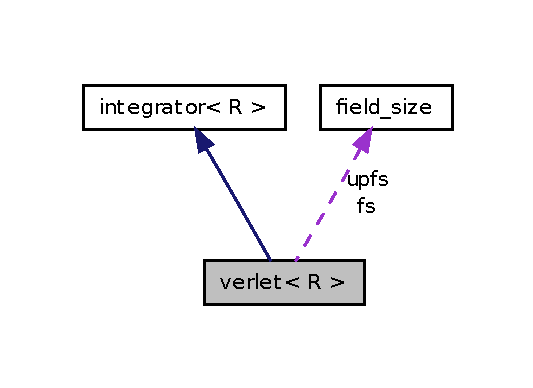
\includegraphics[width=220pt]{classverlet__coll__graph}
\end{center}
\end{figure}
\subsection*{Public Member Functions}
\begin{DoxyCompactItemize}
\item 
\hypertarget{classverlet_a1a51977dc9b12a64728c566c1f7278a5}{
{\bfseries verlet} (\hyperlink{structfield__size}{field\_\-size} \&fs\_\-, \hyperlink{structmodel__params}{model\_\-params}$<$ R $>$ \&mp\_\-, \hyperlink{structtime__state}{time\_\-state}$<$ R $>$ \&ts\_\-, \hyperlink{classfield}{field}$<$ R $>$ \&phi\_\-, \hyperlink{classfield}{field}$<$ R $>$ \&phidot\_\-, \hyperlink{classfield}{field}$<$ R $>$ \&chi\_\-, \hyperlink{classfield}{field}$<$ R $>$ \&chidot\_\-)}
\label{classverlet_a1a51977dc9b12a64728c566c1f7278a5}

\item 
\hypertarget{classverlet_aec84a4b02a724f576a230cf82f5de6c1}{
virtual void {\bfseries step} ()}
\label{classverlet_aec84a4b02a724f576a230cf82f5de6c1}

\item 
\hypertarget{classverlet_a2d3949c36534110a43b25184936282b5}{
virtual void {\bfseries initialize} ()}
\label{classverlet_a2d3949c36534110a43b25184936282b5}

\end{DoxyCompactItemize}
\subsection*{Protected Attributes}
\begin{DoxyCompactItemize}
\item 
\hypertarget{classverlet_a8132944cb5e2f0262405f6dd524ec744}{
\hyperlink{structfield__size}{field\_\-size} \& {\bfseries fs}}
\label{classverlet_a8132944cb5e2f0262405f6dd524ec744}

\item 
\hypertarget{classverlet_ab18846ba3ae3b1ab168bade6a1ee9d7f}{
\hyperlink{structfield__size}{field\_\-size} {\bfseries upfs}}
\label{classverlet_ab18846ba3ae3b1ab168bade6a1ee9d7f}

\item 
\hypertarget{classverlet_ade18671af39b471461764f03005fa40a}{
\hyperlink{structmodel__params}{model\_\-params}$<$ R $>$ \& {\bfseries mp}}
\label{classverlet_ade18671af39b471461764f03005fa40a}

\item 
\hypertarget{classverlet_ad63e006c557e397ca7bcdd3f1e03557d}{
\hyperlink{structtime__state}{time\_\-state}$<$ R $>$ \& {\bfseries ts}}
\label{classverlet_ad63e006c557e397ca7bcdd3f1e03557d}

\item 
\hypertarget{classverlet_a5a3951561b39cdaa34f8dd4edf67b615}{
\hyperlink{classfield}{field}$<$ R $>$ \& {\bfseries phi}}
\label{classverlet_a5a3951561b39cdaa34f8dd4edf67b615}

\item 
\hypertarget{classverlet_ac1e282cafe2b4fdf5c7236b4cf563a68}{
\hyperlink{classfield}{field}$<$ R $>$ \& {\bfseries phidot}}
\label{classverlet_ac1e282cafe2b4fdf5c7236b4cf563a68}

\item 
\hypertarget{classverlet_a343a04d465d21ccded427b547127ac39}{
\hyperlink{classfield}{field}$<$ R $>$ \& {\bfseries chi}}
\label{classverlet_a343a04d465d21ccded427b547127ac39}

\item 
\hypertarget{classverlet_a47fcf63465cf28937dbf891fcda013b4}{
\hyperlink{classfield}{field}$<$ R $>$ \& {\bfseries chidot}}
\label{classverlet_a47fcf63465cf28937dbf891fcda013b4}

\item 
\hypertarget{classverlet_a2edeaea57fd000dbff25afef8b9669b7}{
\hyperlink{classfield}{field}$<$ R $>$ {\bfseries phiddot}}
\label{classverlet_a2edeaea57fd000dbff25afef8b9669b7}

\item 
\hypertarget{classverlet_a9f51b2f4d36a34414c014769b4304f4d}{
\hyperlink{classfield}{field}$<$ R $>$ {\bfseries phidot\_\-staggered}}
\label{classverlet_a9f51b2f4d36a34414c014769b4304f4d}

\item 
\hypertarget{classverlet_a52b954790a191420281577f1481e2863}{
\hyperlink{classfield}{field}$<$ R $>$ {\bfseries chiddot}}
\label{classverlet_a52b954790a191420281577f1481e2863}

\item 
\hypertarget{classverlet_a1e7cf84578e28a0c095c63b5d41c7449}{
\hyperlink{classfield}{field}$<$ R $>$ {\bfseries chidot\_\-staggered}}
\label{classverlet_a1e7cf84578e28a0c095c63b5d41c7449}

\item 
\hypertarget{classverlet_a232564ebeb528c9b52bbcc9daa81a909}{
\hyperlink{classnonlinear__transformer}{nonlinear\_\-transformer}$<$ R $>$ {\bfseries nlt}}
\label{classverlet_a232564ebeb528c9b52bbcc9daa81a909}

\item 
\hypertarget{classverlet_ac95f577e1f80514aec3c3f411a3d7e9c}{
\hyperlink{classv__integrator}{v\_\-integrator}$<$ R $>$ {\bfseries vi}}
\label{classverlet_ac95f577e1f80514aec3c3f411a3d7e9c}

\item 
\hypertarget{classverlet_ac46576e82d8a3e2b17a4e592ddaf6b19}{
R {\bfseries addot}}
\label{classverlet_ac46576e82d8a3e2b17a4e592ddaf6b19}

\item 
\hypertarget{classverlet_af978fa48d0bb1330d1648feba4259932}{
R {\bfseries adot\_\-staggered}}
\label{classverlet_af978fa48d0bb1330d1648feba4259932}

\item 
\hypertarget{classverlet_ae72e40fbb1555485c8dbe933b1149936}{
R {\bfseries dptdt}}
\label{classverlet_ae72e40fbb1555485c8dbe933b1149936}

\item 
\hypertarget{classverlet_a0903fd982ba22200c926aa8a6ccb3f2a}{
R {\bfseries ddptdt}}
\label{classverlet_a0903fd982ba22200c926aa8a6ccb3f2a}

\item 
\hypertarget{classverlet_ade5082a86641198153fad5aad8be887c}{
R {\bfseries dptdt\_\-staggered}}
\label{classverlet_ade5082a86641198153fad5aad8be887c}

\end{DoxyCompactItemize}
\subsubsection*{template$<$typename R$>$ class verlet$<$ R $>$}



The documentation for this class was generated from the following files:\begin{DoxyCompactItemize}
\item 
\hyperlink{verlet_8hpp}{verlet.hpp}\item 
verlet.cpp\end{DoxyCompactItemize}

\chapter{File Documentation}
\hypertarget{defrost__style__initializer_8hpp}{
\section{defrost\_\-style\_\-initializer.hpp File Reference}
\label{defrost__style__initializer_8hpp}\index{defrost\_\-style\_\-initializer.hpp@{defrost\_\-style\_\-initializer.hpp}}
}


DEFROST-\/style initial conditions.  
{\ttfamily \#include \char`\"{}field\_\-size.hpp\char`\"{}}\par
{\ttfamily \#include \char`\"{}model\_\-params.hpp\char`\"{}}\par
{\ttfamily \#include \char`\"{}field.hpp\char`\"{}}\par
{\ttfamily \#include \char`\"{}initializer.hpp\char`\"{}}\par
Include dependency graph for defrost\_\-style\_\-initializer.hpp:\nopagebreak
\begin{figure}[H]
\begin{center}
\leavevmode
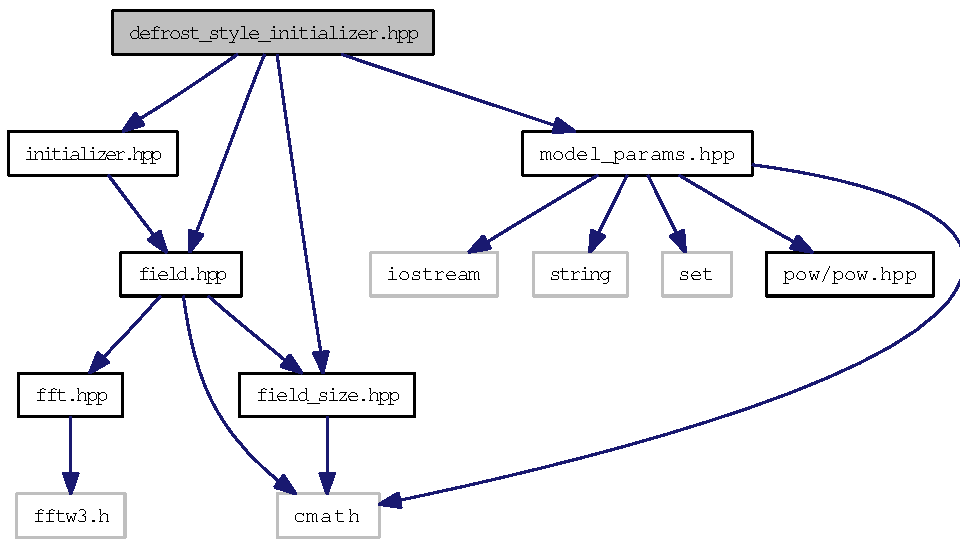
\includegraphics[width=248pt]{defrost__style__initializer_8hpp__incl}
\end{center}
\end{figure}
\subsection*{Classes}
\begin{DoxyCompactItemize}
\item 
class \hyperlink{classdefrost__style__initializer}{defrost\_\-style\_\-initializer$<$ R $>$}
\begin{DoxyCompactList}\small\item\em DEFROST-\/style initial conditions. \item\end{DoxyCompactList}\end{DoxyCompactItemize}


\subsection{Detailed Description}
DEFROST-\/style initial conditions. 
\hypertarget{energy__outputter_8hpp}{
\section{energy\_\-outputter.hpp File Reference}
\label{energy__outputter_8hpp}\index{energy\_\-outputter.hpp@{energy\_\-outputter.hpp}}
}


Outputter for the energy TSV file.  


{\ttfamily \#include \char`\"{}field.hpp\char`\"{}}\par
{\ttfamily \#include \char`\"{}model\_\-params.hpp\char`\"{}}\par
{\ttfamily \#include \char`\"{}time\_\-state.hpp\char`\"{}}\par
{\ttfamily \#include \char`\"{}v\_\-integrator.hpp\char`\"{}}\par
{\ttfamily \#include $<$iostream$>$}\par
{\ttfamily \#include $<$fstream$>$}\par
Include dependency graph for energy\_\-outputter.hpp:
\nopagebreak
\begin{figure}[H]
\begin{center}
\leavevmode
\includegraphics[width=400pt]{energy__outputter_8hpp__incl}
\end{center}
\end{figure}
\subsection*{Classes}
\begin{DoxyCompactItemize}
\item 
class \hyperlink{classenergy__outputter}{energy\_\-outputter$<$ R $>$}
\begin{DoxyCompactList}\small\item\em Outputter for the energy TSV file. \item\end{DoxyCompactList}\end{DoxyCompactItemize}


\subsection{Detailed Description}
Outputter for the energy TSV file. 
\hypertarget{fft_8hpp}{
\section{fft.hpp File Reference}
\label{fft_8hpp}\index{fft.hpp@{fft.hpp}}
}


FFT wrappers.  
{\ttfamily \#include $<$fftw3.h$>$}\par
Include dependency graph for fft.hpp:\nopagebreak
\begin{figure}[H]
\begin{center}
\leavevmode
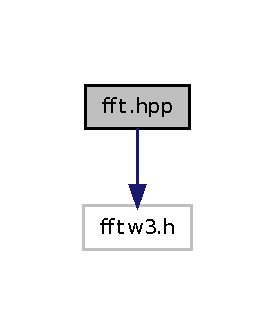
\includegraphics[width=48pt]{fft_8hpp__incl}
\end{center}
\end{figure}
This graph shows which files directly or indirectly include this file:\nopagebreak
\begin{figure}[H]
\begin{center}
\leavevmode
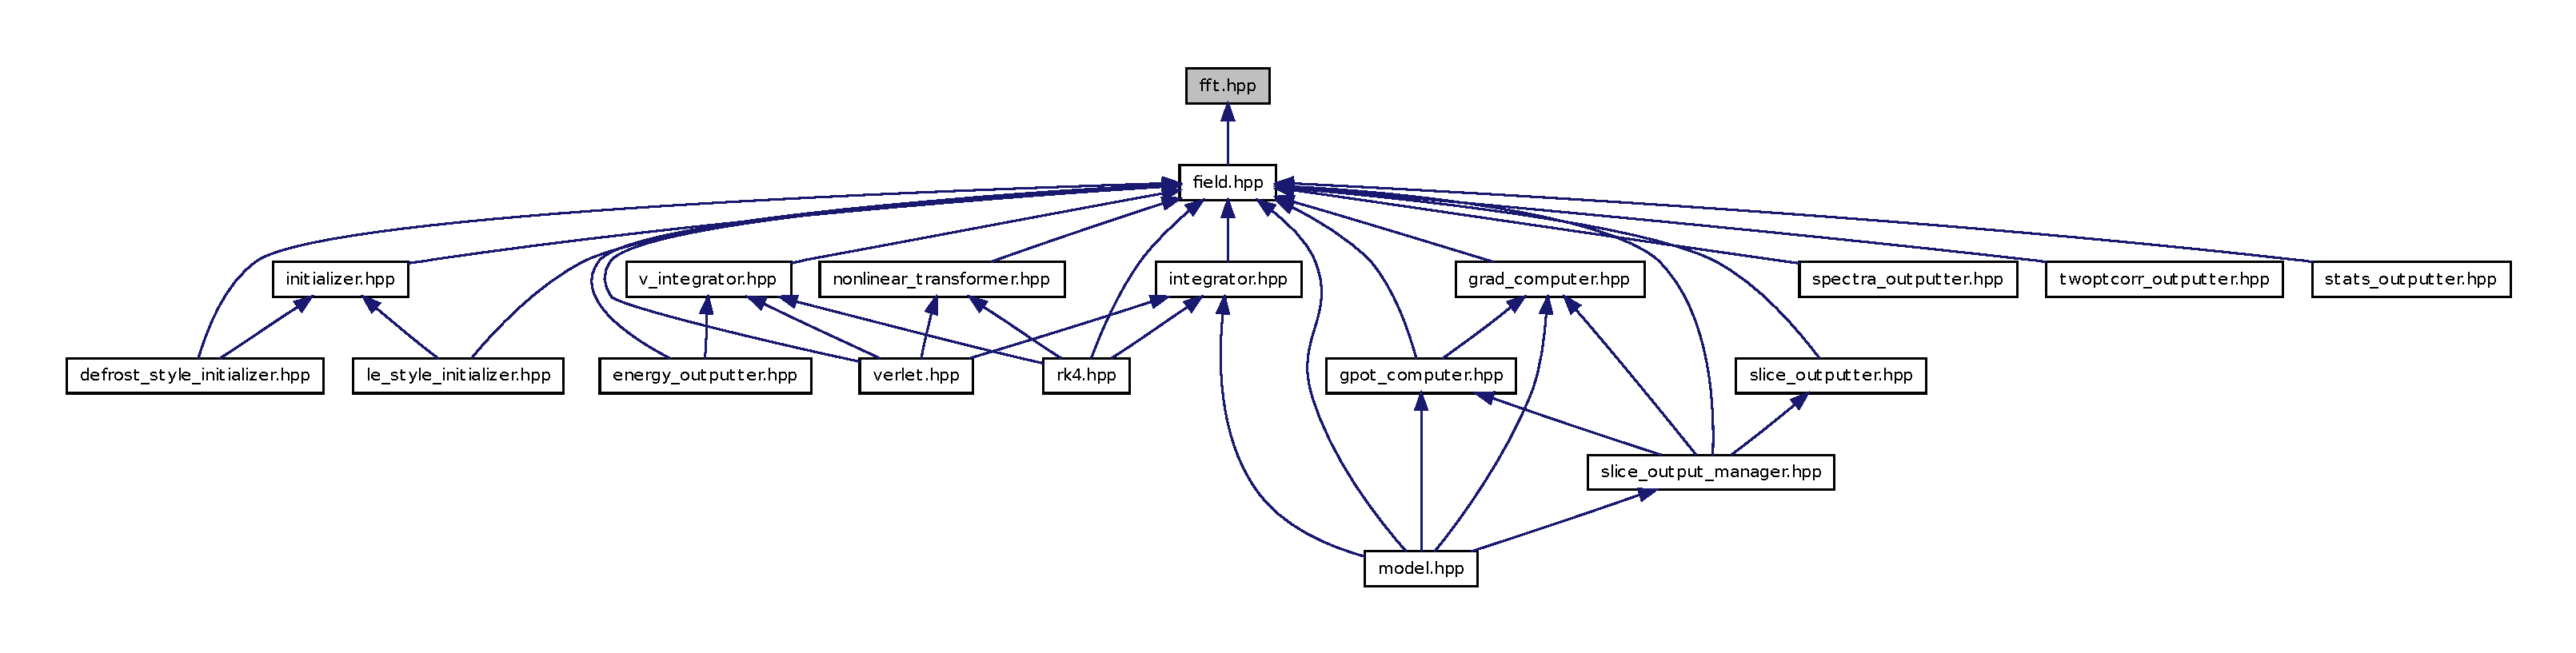
\includegraphics[width=420pt]{fft_8hpp__dep__incl}
\end{center}
\end{figure}
\subsection*{Classes}
\begin{DoxyCompactItemize}
\item 
class \hyperlink{classfft__r2r__1d__plan}{fft\_\-r2r\_\-1d\_\-plan$<$ R $>$}
\item 
class \hyperlink{classfft__r2r__1d__plan_3_01double_01_4}{fft\_\-r2r\_\-1d\_\-plan$<$ double $>$}
\item 
class \hyperlink{classfft__dft__c2r__3d__plan}{fft\_\-dft\_\-c2r\_\-3d\_\-plan$<$ R $>$}
\item 
class \hyperlink{classfft__dft__c2r__3d__plan_3_01double_01_4}{fft\_\-dft\_\-c2r\_\-3d\_\-plan$<$ double $>$}
\item 
class \hyperlink{classfft__dft__r2c__3d__plan}{fft\_\-dft\_\-r2c\_\-3d\_\-plan$<$ R $>$}
\item 
class \hyperlink{classfft__dft__r2c__3d__plan_3_01double_01_4}{fft\_\-dft\_\-r2c\_\-3d\_\-plan$<$ double $>$}
\end{DoxyCompactItemize}
\subsection*{Enumerations}
\begin{DoxyCompactItemize}
\item 
enum {\bfseries fft\_\-r2r\_\-kind} \{ \par
{\bfseries r2hc} =  FFTW\_\-R2HC, 
{\bfseries hc2r} =  FFTW\_\-HC2R, 
{\bfseries dht} =  FFTW\_\-DHT, 
{\bfseries redft00} =  FFTW\_\-REDFT00, 
\par
{\bfseries redft10} =  FFTW\_\-REDFT10, 
{\bfseries redft01} =  FFTW\_\-REDFT01, 
{\bfseries redft11} =  FFTW\_\-REDFT11, 
{\bfseries rodft00} =  FFTW\_\-RODFT00, 
\par
{\bfseries rodft10} =  FFTW\_\-RODFT10, 
{\bfseries rodft01} =  FFTW\_\-RODFT01, 
{\bfseries rodft11} =  FFTW\_\-RODFT11
 \}
\end{DoxyCompactItemize}
\subsection*{Functions}
\begin{DoxyCompactItemize}
\item 
\hypertarget{fft_8hpp_a45c093a4e007c43e392814a8ac6a262d}{
{\footnotesize template$<$typename R $>$ }\\R $\ast$ {\bfseries fft\_\-malloc} (size\_\-t sz)}
\label{fft_8hpp_a45c093a4e007c43e392814a8ac6a262d}

\item 
\hypertarget{fft_8hpp_a7834b27b8f324419b97af591726d9f08}{
{\footnotesize template$<$$>$ }\\double $\ast$ {\bfseries fft\_\-malloc$<$ double $>$} (size\_\-t sz)}
\label{fft_8hpp_a7834b27b8f324419b97af591726d9f08}

\item 
\hypertarget{fft_8hpp_adf5f200ea21dff70c558a0b21fe844dc}{
{\footnotesize template$<$typename R $>$ }\\void {\bfseries fft\_\-free} (R $\ast$ptr)}
\label{fft_8hpp_adf5f200ea21dff70c558a0b21fe844dc}

\item 
\hypertarget{fft_8hpp_a745a5f2046fbafdfcab7a5dc47bb4894}{
{\footnotesize template$<$$>$ }\\void {\bfseries fft\_\-free$<$ double $>$} (double $\ast$ptr)}
\label{fft_8hpp_a745a5f2046fbafdfcab7a5dc47bb4894}

\end{DoxyCompactItemize}


\subsection{Detailed Description}
FFT wrappers. 
\hypertarget{field_8hpp}{
\section{field.hpp File Reference}
\label{field_8hpp}\index{field.hpp@{field.hpp}}
}


Three-\/dimensional scalar fields.  
{\ttfamily \#include \char`\"{}fft.hpp\char`\"{}}\par
{\ttfamily \#include \char`\"{}field\_\-size.hpp\char`\"{}}\par
{\ttfamily \#include $<$cmath$>$}\par
Include dependency graph for field.hpp:\nopagebreak
\begin{figure}[H]
\begin{center}
\leavevmode
\includegraphics[width=107pt]{field_8hpp__incl}
\end{center}
\end{figure}
This graph shows which files directly or indirectly include this file:\nopagebreak
\begin{figure}[H]
\begin{center}
\leavevmode
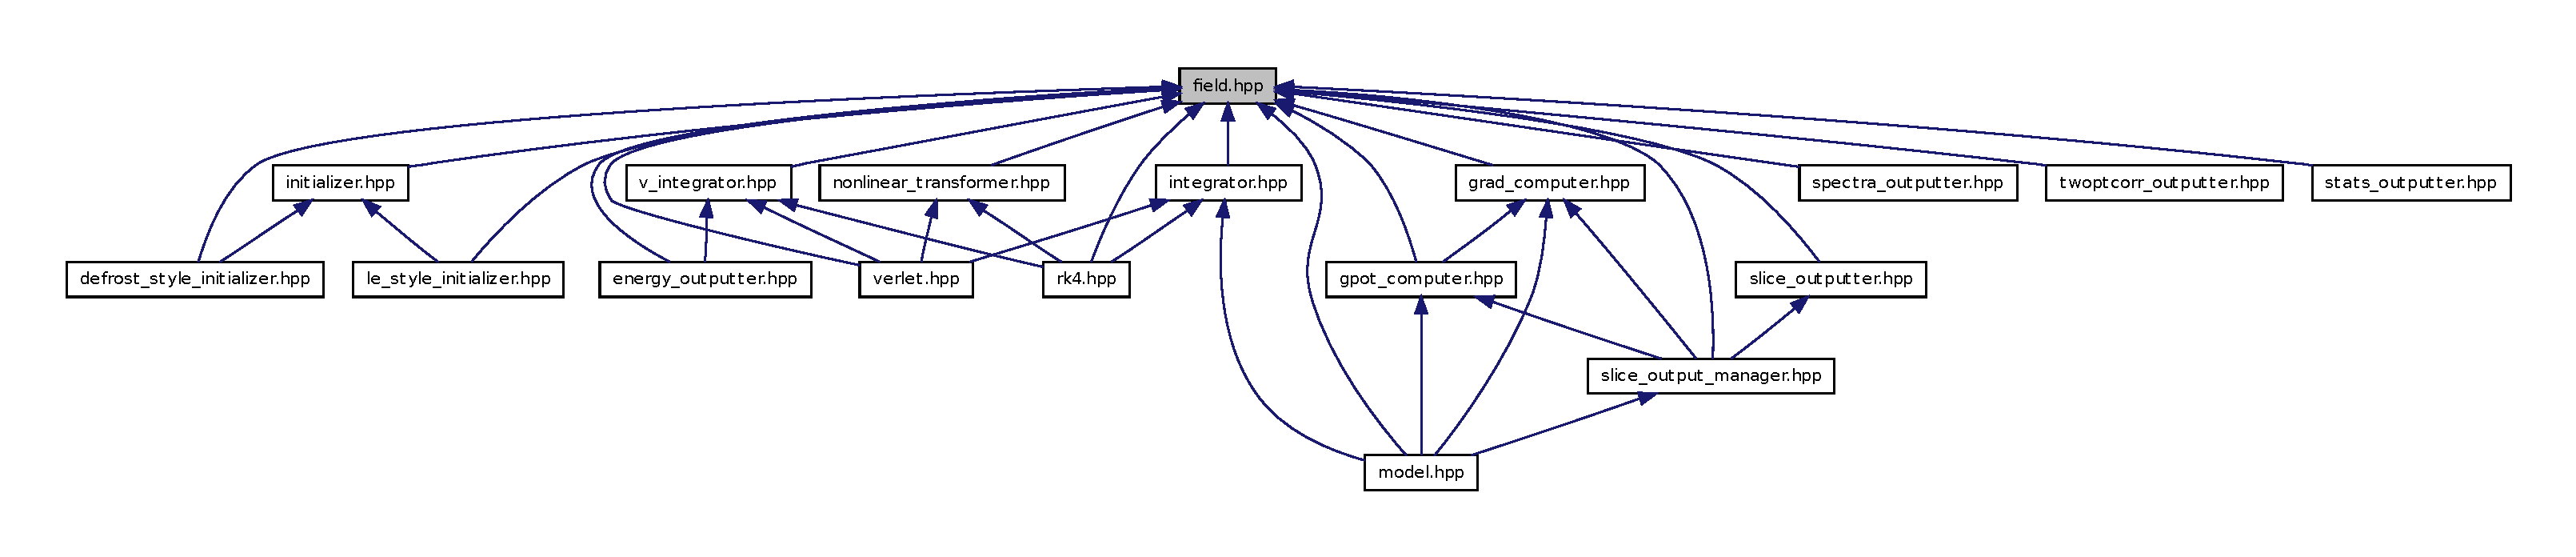
\includegraphics[width=420pt]{field_8hpp__dep__incl}
\end{center}
\end{figure}
\subsection*{Classes}
\begin{DoxyCompactItemize}
\item 
class \hyperlink{classfield}{field$<$ R $>$}
\begin{DoxyCompactList}\small\item\em A three-\/dimensional scalar field in both position and momentum space. \item\end{DoxyCompactList}\end{DoxyCompactItemize}
\subsection*{Enumerations}
\begin{DoxyCompactItemize}
\item 
enum {\bfseries field\_\-state} \{ \par
{\bfseries uninitialized}, 
{\bfseries position}, 
{\bfseries momentum}, 
{\bfseries padded\_\-position}, 
\par
{\bfseries padded\_\-momentum}
 \}
\end{DoxyCompactItemize}


\subsection{Detailed Description}
Three-\/dimensional scalar fields. 
\hypertarget{field__size_8hpp}{
\section{field\_\-size.hpp File Reference}
\label{field__size_8hpp}\index{field\_\-size.hpp@{field\_\-size.hpp}}
}


Field grid size and derived size-\/related quantities.  
{\ttfamily \#include $<$cmath$>$}\par
Include dependency graph for field\_\-size.hpp:\nopagebreak
\begin{figure}[H]
\begin{center}
\leavevmode
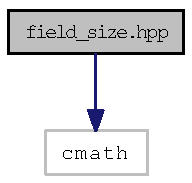
\includegraphics[width=64pt]{field__size_8hpp__incl}
\end{center}
\end{figure}
This graph shows which files directly or indirectly include this file:\nopagebreak
\begin{figure}[H]
\begin{center}
\leavevmode
\includegraphics[width=420pt]{field__size_8hpp__dep__incl}
\end{center}
\end{figure}
\subsection*{Classes}
\begin{DoxyCompactItemize}
\item 
struct \hyperlink{structfield__size}{field\_\-size}
\end{DoxyCompactItemize}


\subsection{Detailed Description}
Field grid size and derived size-\/related quantities. 
\hypertarget{gpot__computer_8hpp}{
\section{gpot\_\-computer.hpp File Reference}
\label{gpot__computer_8hpp}\index{gpot\_\-computer.hpp@{gpot\_\-computer.hpp}}
}


Gravitational-\/potential computations.  
{\ttfamily \#include \char`\"{}field\_\-size.hpp\char`\"{}}\par
{\ttfamily \#include \char`\"{}model\_\-params.hpp\char`\"{}}\par
{\ttfamily \#include \char`\"{}time\_\-state.hpp\char`\"{}}\par
{\ttfamily \#include \char`\"{}field.hpp\char`\"{}}\par
{\ttfamily \#include \char`\"{}grad\_\-computer.hpp\char`\"{}}\par
Include dependency graph for gpot\_\-computer.hpp:\nopagebreak
\begin{figure}[H]
\begin{center}
\leavevmode
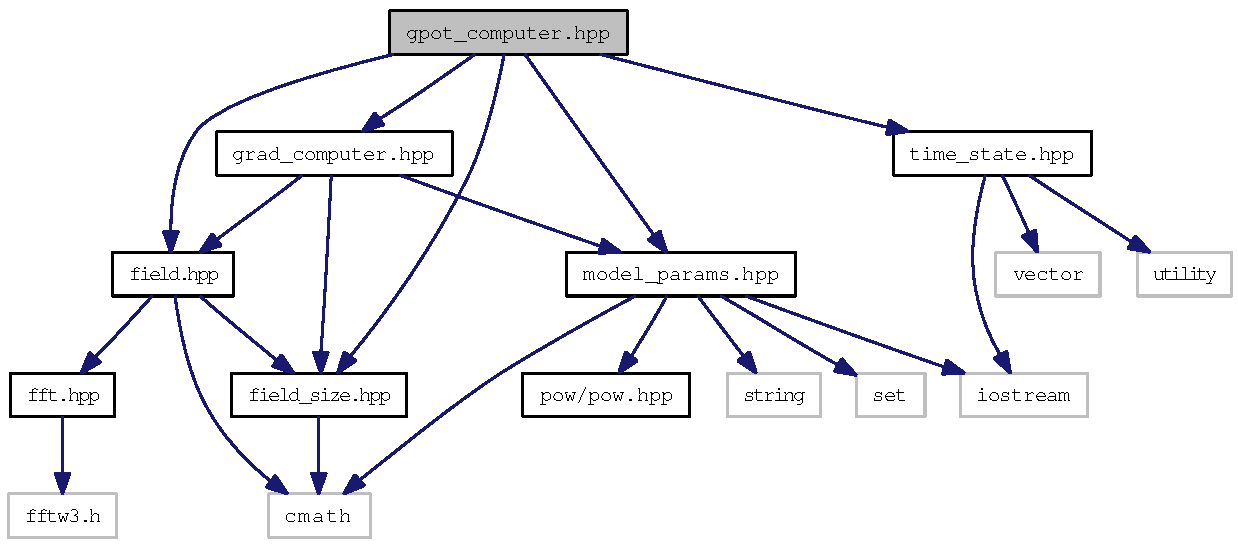
\includegraphics[width=315pt]{gpot__computer_8hpp__incl}
\end{center}
\end{figure}
This graph shows which files directly or indirectly include this file:\nopagebreak
\begin{figure}[H]
\begin{center}
\leavevmode
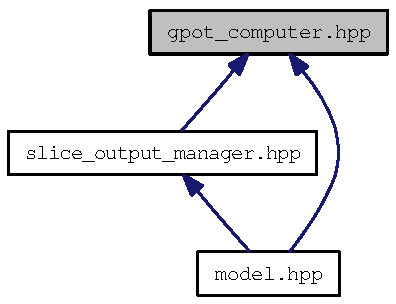
\includegraphics[width=113pt]{gpot__computer_8hpp__dep__incl}
\end{center}
\end{figure}
\subsection*{Classes}
\begin{DoxyCompactItemize}
\item 
class \hyperlink{classgpot__computer}{gpot\_\-computer$<$ R $>$}
\begin{DoxyCompactList}\small\item\em Computer of the gravitational potential from the energy density of the phi and chi fields. \item\end{DoxyCompactList}\end{DoxyCompactItemize}


\subsection{Detailed Description}
Gravitational-\/potential computations. 
\hypertarget{grad__computer_8hpp}{
\section{grad\_\-computer.hpp File Reference}
\label{grad__computer_8hpp}\index{grad\_\-computer.hpp@{grad\_\-computer.hpp}}
}


Computation of the gradient in Fourier space.  


{\ttfamily \#include \char`\"{}field\_\-size.hpp\char`\"{}}\par
{\ttfamily \#include \char`\"{}model\_\-params.hpp\char`\"{}}\par
{\ttfamily \#include \char`\"{}field.hpp\char`\"{}}\par
Include dependency graph for grad\_\-computer.hpp:
\nopagebreak
\begin{figure}[H]
\begin{center}
\leavevmode
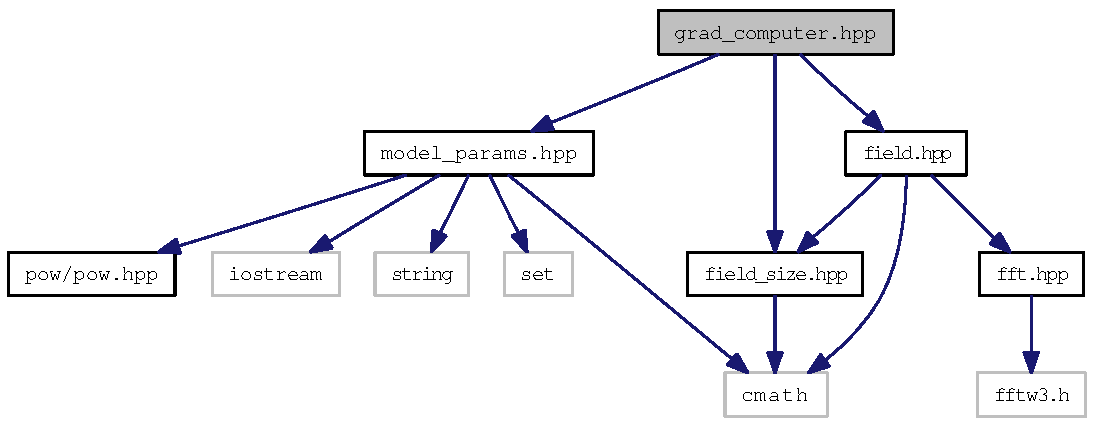
\includegraphics[width=400pt]{grad__computer_8hpp__incl}
\end{center}
\end{figure}
This graph shows which files directly or indirectly include this file:
\nopagebreak
\begin{figure}[H]
\begin{center}
\leavevmode
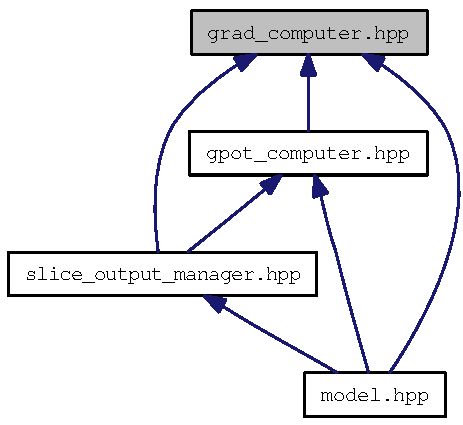
\includegraphics[width=294pt]{grad__computer_8hpp__dep__incl}
\end{center}
\end{figure}
\subsection*{Classes}
\begin{DoxyCompactItemize}
\item 
class \hyperlink{classgrad__computer}{grad\_\-computer$<$ R $>$}
\end{DoxyCompactItemize}


\subsection{Detailed Description}
Computation of the gradient in Fourier space. 
\hypertarget{grid__funcs_8hpp}{
\section{grid\_\-funcs.hpp File Reference}
\label{grid__funcs_8hpp}\index{grid\_\-funcs.hpp@{grid\_\-funcs.hpp}}
}


Grid point functions used for slice output, etc.  
{\ttfamily \#include \char`\"{}pow/pow.hpp\char`\"{}}\par
{\ttfamily \#include \char`\"{}model\_\-params.hpp\char`\"{}}\par
{\ttfamily \#include \char`\"{}field\_\-size.hpp\char`\"{}}\par
{\ttfamily \#include \char`\"{}time\_\-state.hpp\char`\"{}}\par
{\ttfamily \#include $<$cmath$>$}\par
Include dependency graph for grid\_\-funcs.hpp:\nopagebreak
\begin{figure}[H]
\begin{center}
\leavevmode
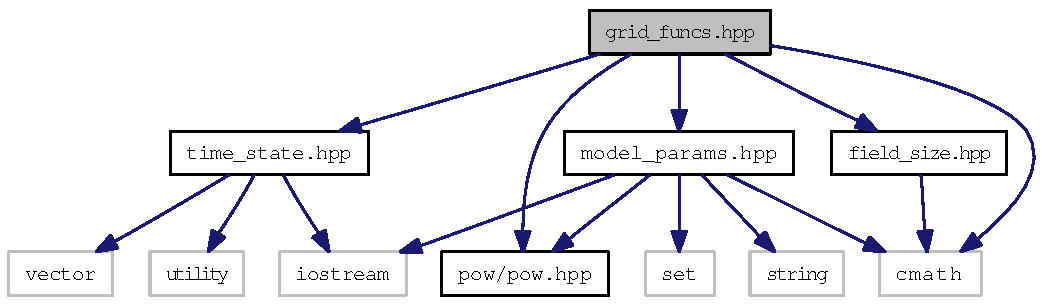
\includegraphics[width=268pt]{grid__funcs_8hpp__incl}
\end{center}
\end{figure}
\subsection*{Classes}
\begin{DoxyCompactItemize}
\item 
struct \hyperlink{structgrid__funcs}{grid\_\-funcs$<$ R $>$}
\end{DoxyCompactItemize}


\subsection{Detailed Description}
Grid point functions used for slice output, etc. 
\hypertarget{initializer_8hpp}{
\section{initializer.hpp File Reference}
\label{initializer_8hpp}\index{initializer.hpp@{initializer.hpp}}
}


Generic field-\/initialization.  


{\ttfamily \#include \char`\"{}field.hpp\char`\"{}}\par
Include dependency graph for initializer.hpp:
\nopagebreak
\begin{figure}[H]
\begin{center}
\leavevmode
\includegraphics[width=250pt]{initializer_8hpp__incl}
\end{center}
\end{figure}
This graph shows which files directly or indirectly include this file:
\nopagebreak
\begin{figure}[H]
\begin{center}
\leavevmode
\includegraphics[width=378pt]{initializer_8hpp__dep__incl}
\end{center}
\end{figure}
\subsection*{Classes}
\begin{DoxyCompactItemize}
\item 
class \hyperlink{classinitializer}{initializer$<$ R $>$}
\end{DoxyCompactItemize}


\subsection{Detailed Description}
Generic field-\/initialization. 
\hypertarget{integrator_8hpp}{
\section{integrator.hpp File Reference}
\label{integrator_8hpp}\index{integrator.hpp@{integrator.hpp}}
}


Generic time-\/step evolution.  
{\ttfamily \#include \char`\"{}field\_\-size.hpp\char`\"{}}\par
{\ttfamily \#include \char`\"{}model\_\-params.hpp\char`\"{}}\par
{\ttfamily \#include \char`\"{}field.hpp\char`\"{}}\par
Include dependency graph for integrator.hpp:\nopagebreak
\begin{figure}[H]
\begin{center}
\leavevmode
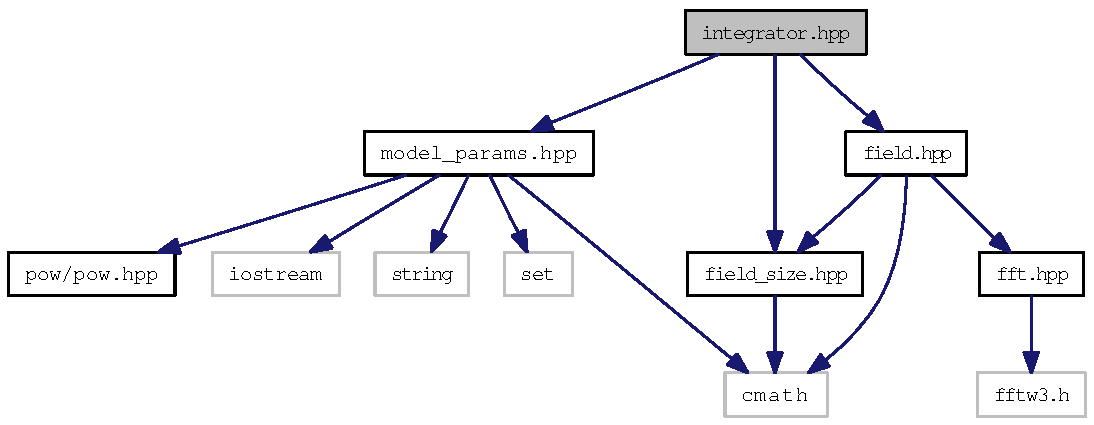
\includegraphics[width=280pt]{integrator_8hpp__incl}
\end{center}
\end{figure}
This graph shows which files directly or indirectly include this file:\nopagebreak
\begin{figure}[H]
\begin{center}
\leavevmode
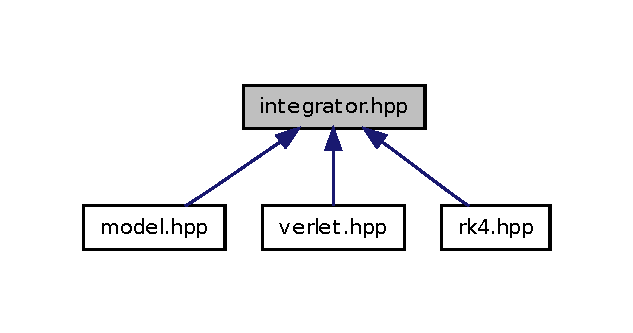
\includegraphics[width=134pt]{integrator_8hpp__dep__incl}
\end{center}
\end{figure}
\subsection*{Classes}
\begin{DoxyCompactItemize}
\item 
class \hyperlink{classintegrator}{integrator$<$ R $>$}
\end{DoxyCompactItemize}


\subsection{Detailed Description}
Generic time-\/step evolution. 
\hypertarget{le__style__initializer_8hpp}{
\section{le\_\-style\_\-initializer.hpp File Reference}
\label{le__style__initializer_8hpp}\index{le\_\-style\_\-initializer.hpp@{le\_\-style\_\-initializer.hpp}}
}


LatticeEasy-\/style initialization.  


{\ttfamily \#include \char`\"{}field\_\-size.hpp\char`\"{}}\par
{\ttfamily \#include \char`\"{}model\_\-params.hpp\char`\"{}}\par
{\ttfamily \#include \char`\"{}field.hpp\char`\"{}}\par
{\ttfamily \#include \char`\"{}initializer.hpp\char`\"{}}\par
{\ttfamily \#include $<$cmath$>$}\par
Include dependency graph for le\_\-style\_\-initializer.hpp:
\nopagebreak
\begin{figure}[H]
\begin{center}
\leavevmode
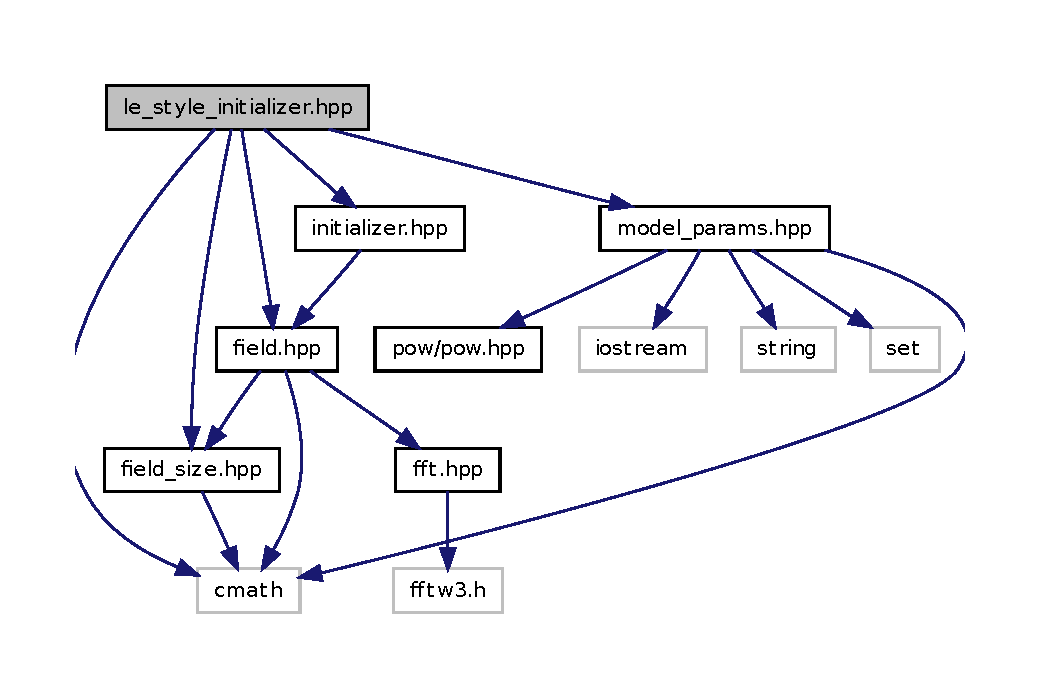
\includegraphics[width=400pt]{le__style__initializer_8hpp__incl}
\end{center}
\end{figure}
\subsection*{Classes}
\begin{DoxyCompactItemize}
\item 
class \hyperlink{classle__style__initializer}{le\_\-style\_\-initializer$<$ R $>$}
\end{DoxyCompactItemize}


\subsection{Detailed Description}
LatticeEasy-\/style initialization. 
\hypertarget{model_8hpp}{
\section{model.hpp File Reference}
\label{model_8hpp}\index{model.hpp@{model.hpp}}
}


A particular simulated situation.  


{\ttfamily \#include \char`\"{}field\_\-size.hpp\char`\"{}}\par
{\ttfamily \#include \char`\"{}model\_\-params.hpp\char`\"{}}\par
{\ttfamily \#include \char`\"{}time\_\-state.hpp\char`\"{}}\par
{\ttfamily \#include \char`\"{}field.hpp\char`\"{}}\par
{\ttfamily \#include \char`\"{}integrator.hpp\char`\"{}}\par
{\ttfamily \#include \char`\"{}slice\_\-output\_\-manager.hpp\char`\"{}}\par
{\ttfamily \#include \char`\"{}grad\_\-computer.hpp\char`\"{}}\par
{\ttfamily \#include \char`\"{}gpot\_\-computer.hpp\char`\"{}}\par
Include dependency graph for model.hpp:
\nopagebreak
\begin{figure}[H]
\begin{center}
\leavevmode
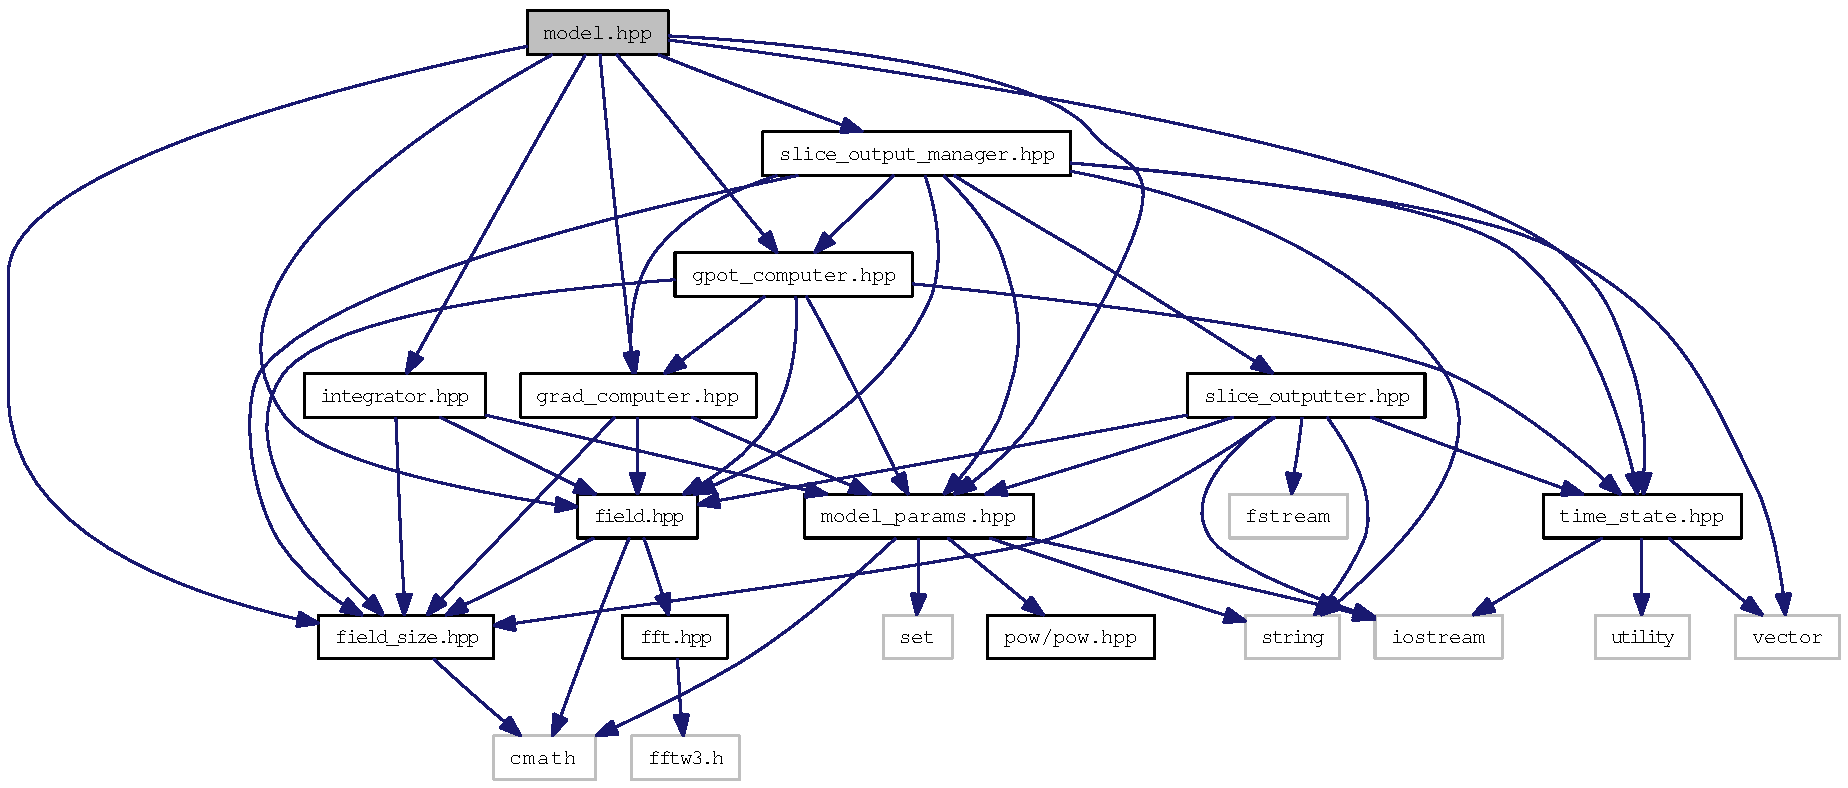
\includegraphics[width=400pt]{model_8hpp__incl}
\end{center}
\end{figure}
\subsection*{Classes}
\begin{DoxyCompactItemize}
\item 
class \hyperlink{classmodel}{model$<$ R $>$}
\end{DoxyCompactItemize}


\subsection{Detailed Description}
A particular simulated situation. 
\hypertarget{model__params_8hpp}{
\section{model\_\-params.hpp File Reference}
\label{model__params_8hpp}\index{model\_\-params.hpp@{model\_\-params.hpp}}
}


The physical model parameters.  


{\ttfamily \#include \char`\"{}pow/pow.hpp\char`\"{}}\par
{\ttfamily \#include $<$iostream$>$}\par
{\ttfamily \#include $<$string$>$}\par
{\ttfamily \#include $<$set$>$}\par
{\ttfamily \#include $<$cmath$>$}\par
Include dependency graph for model\_\-params.hpp:
\nopagebreak
\begin{figure}[H]
\begin{center}
\leavevmode
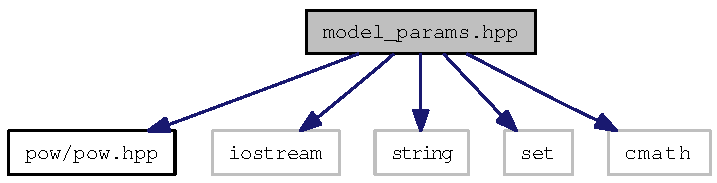
\includegraphics[width=400pt]{model__params_8hpp__incl}
\end{center}
\end{figure}
This graph shows which files directly or indirectly include this file:
\nopagebreak
\begin{figure}[H]
\begin{center}
\leavevmode
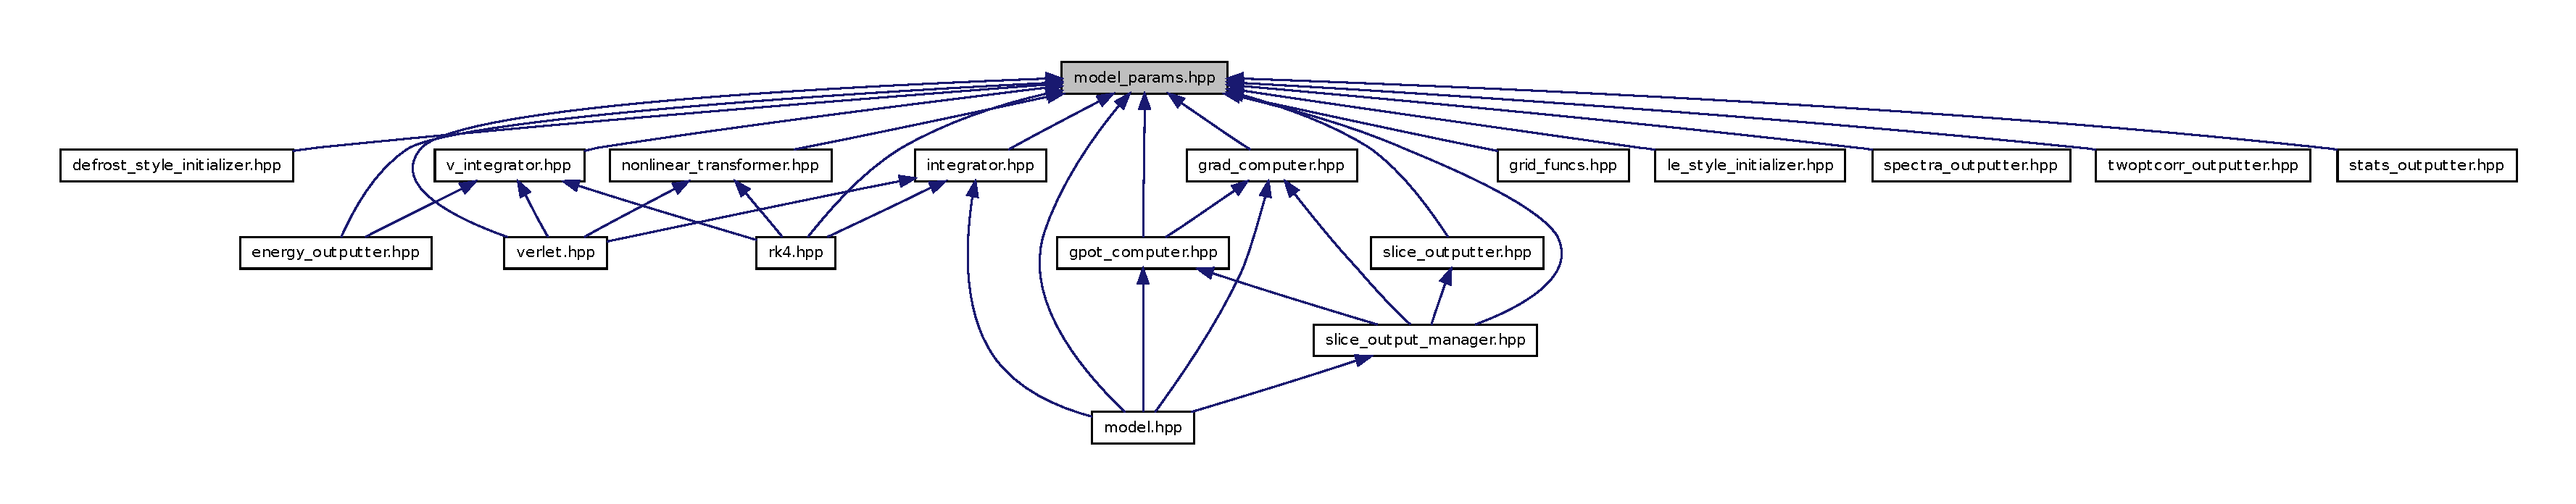
\includegraphics[width=400pt]{model__params_8hpp__dep__incl}
\end{center}
\end{figure}
\subsection*{Classes}
\begin{DoxyCompactItemize}
\item 
struct \hyperlink{structrs__init}{rs\_\-init$<$ R $>$}
\item 
struct \hyperlink{structmodel__params}{model\_\-params$<$ R $>$}
\begin{DoxyCompactList}\small\item\em Static model parameters. \item\end{DoxyCompactList}\end{DoxyCompactItemize}
\subsection*{Functions}
\begin{DoxyCompactItemize}
\item 
\hypertarget{model__params_8hpp_a950dee6bab2b45c6d2d7a2d7cb332467}{
{\footnotesize template$<$typename R $>$ }\\bool {\bfseries operator$<$} (const \hyperlink{structrs__init}{rs\_\-init}$<$ R $>$ \&rs1, const \hyperlink{structrs__init}{rs\_\-init}$<$ R $>$ \&rs2)}
\label{model__params_8hpp_a950dee6bab2b45c6d2d7a2d7cb332467}

\end{DoxyCompactItemize}


\subsection{Detailed Description}
The physical model parameters. 
\hypertarget{nonlinear__transformer_8hpp}{
\section{nonlinear\_\-transformer.hpp File Reference}
\label{nonlinear__transformer_8hpp}\index{nonlinear\_\-transformer.hpp@{nonlinear\_\-transformer.hpp}}
}


Momentum-\/space representations of nonlinear field terms.  


{\ttfamily \#include \char`\"{}field\_\-size.hpp\char`\"{}}\par
{\ttfamily \#include \char`\"{}model\_\-params.hpp\char`\"{}}\par
{\ttfamily \#include \char`\"{}field.hpp\char`\"{}}\par
{\ttfamily \#include \char`\"{}time\_\-state.hpp\char`\"{}}\par
Include dependency graph for nonlinear\_\-transformer.hpp:
\nopagebreak
\begin{figure}[H]
\begin{center}
\leavevmode
\includegraphics[width=400pt]{nonlinear__transformer_8hpp__incl}
\end{center}
\end{figure}
This graph shows which files directly or indirectly include this file:
\nopagebreak
\begin{figure}[H]
\begin{center}
\leavevmode
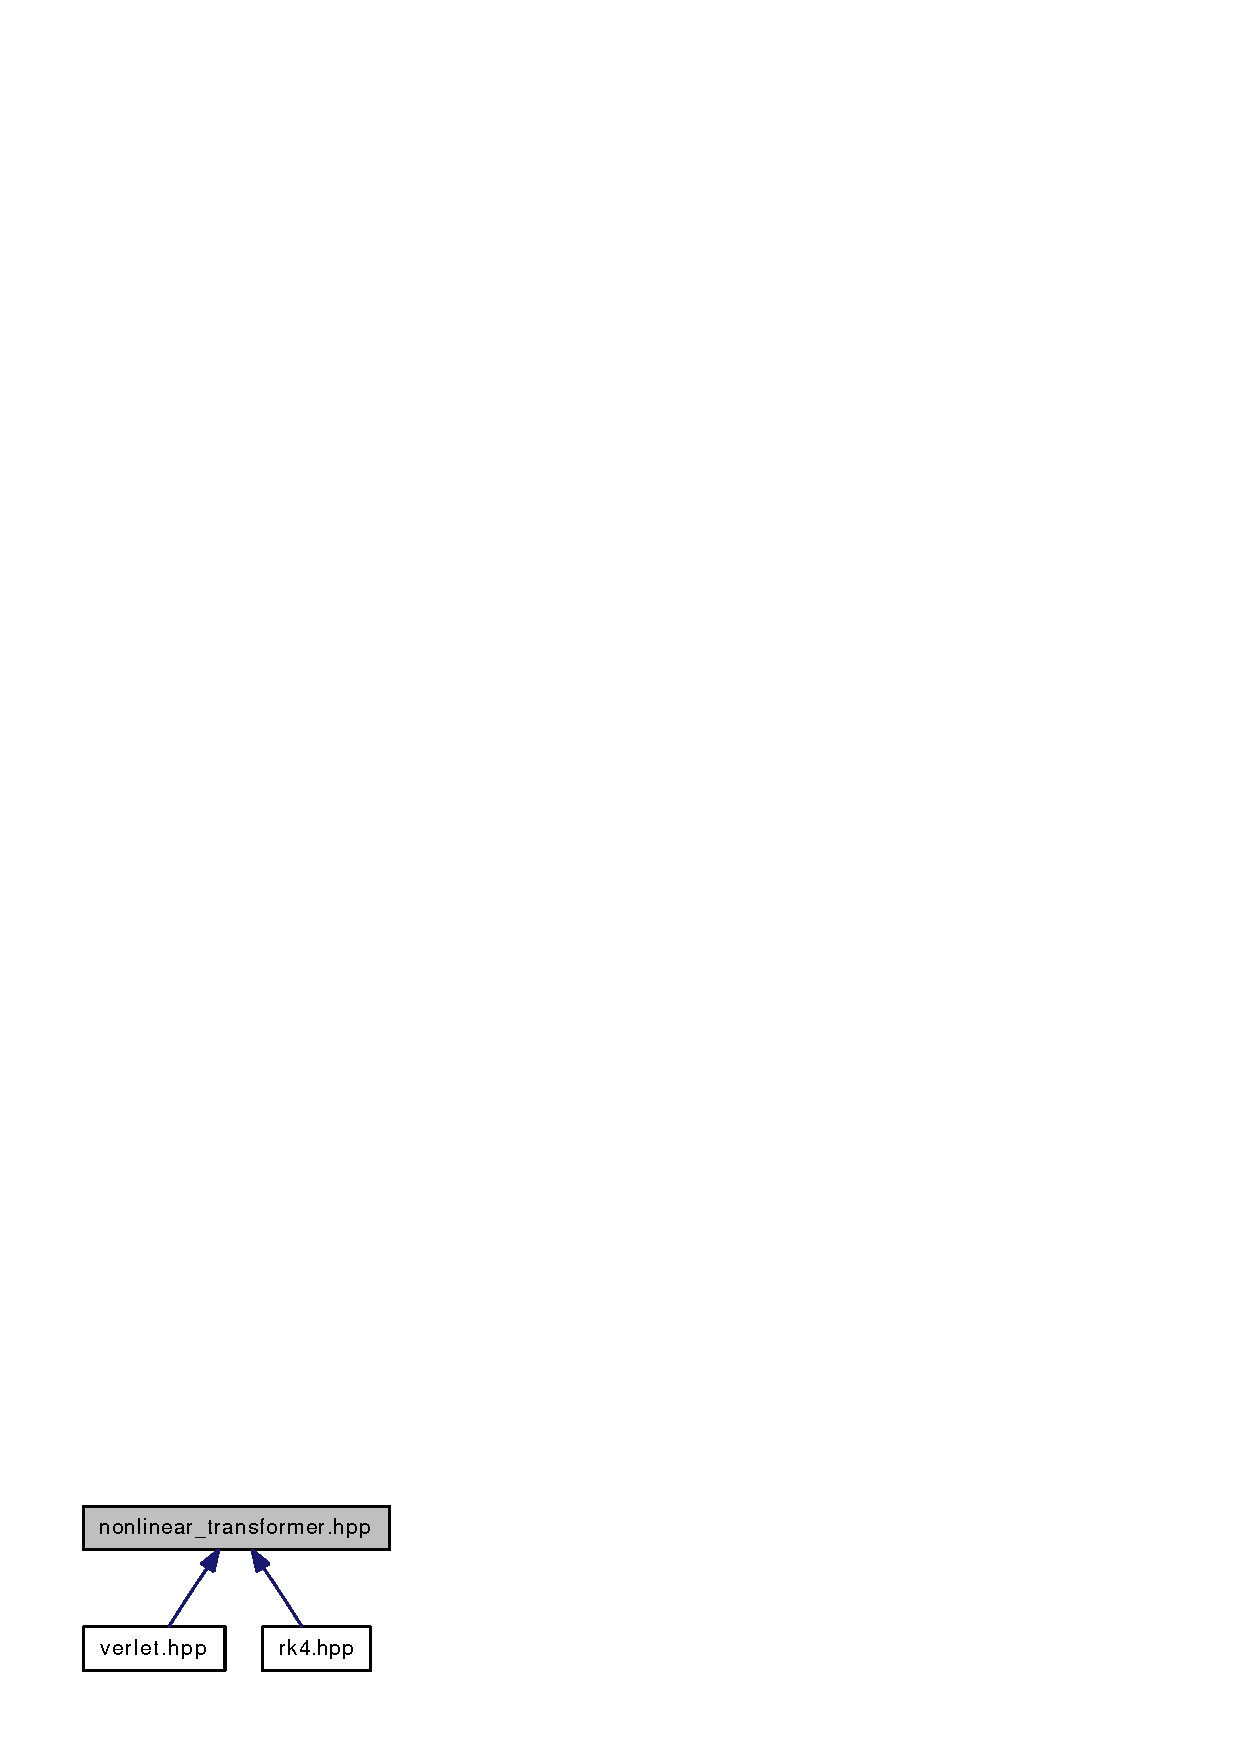
\includegraphics[width=226pt]{nonlinear__transformer_8hpp__dep__incl}
\end{center}
\end{figure}
\subsection*{Classes}
\begin{DoxyCompactItemize}
\item 
class \hyperlink{classnonlinear__transformer}{nonlinear\_\-transformer$<$ R $>$}
\end{DoxyCompactItemize}


\subsection{Detailed Description}
Momentum-\/space representations of nonlinear field terms. 
\hypertarget{pow_8hpp}{
\section{pow/pow.hpp File Reference}
\label{pow_8hpp}\index{pow/pow.hpp@{pow/pow.hpp}}
}


Template function to compute the integer power of its argument.  


This graph shows which files directly or indirectly include this file:
\nopagebreak
\begin{figure}[H]
\begin{center}
\leavevmode
\includegraphics[width=400pt]{pow_8hpp__dep__incl}
\end{center}
\end{figure}


\subsection{Detailed Description}
Template function to compute the integer power of its argument. 
\hypertarget{rk4_8hpp}{
\section{rk4.hpp File Reference}
\label{rk4_8hpp}\index{rk4.hpp@{rk4.hpp}}
}


Fourth-\/order Runge–Kutta (RK4) integrator.  


{\ttfamily \#include \char`\"{}field\_\-size.hpp\char`\"{}}\par
{\ttfamily \#include \char`\"{}model\_\-params.hpp\char`\"{}}\par
{\ttfamily \#include \char`\"{}time\_\-state.hpp\char`\"{}}\par
{\ttfamily \#include \char`\"{}field.hpp\char`\"{}}\par
{\ttfamily \#include \char`\"{}integrator.hpp\char`\"{}}\par
{\ttfamily \#include \char`\"{}nonlinear\_\-transformer.hpp\char`\"{}}\par
{\ttfamily \#include \char`\"{}v\_\-integrator.hpp\char`\"{}}\par
Include dependency graph for rk4.hpp:
\nopagebreak
\begin{figure}[H]
\begin{center}
\leavevmode
\includegraphics[width=400pt]{rk4_8hpp__incl}
\end{center}
\end{figure}
\subsection*{Classes}
\begin{DoxyCompactItemize}
\item 
class \hyperlink{classrk4}{rk4$<$ R $>$}
\end{DoxyCompactItemize}


\subsection{Detailed Description}
Fourth-\/order Runge–Kutta (RK4) integrator. 
\hypertarget{slice__output__manager_8hpp}{
\section{slice\_\-output\_\-manager.hpp File Reference}
\label{slice__output__manager_8hpp}\index{slice\_\-output\_\-manager.hpp@{slice\_\-output\_\-manager.hpp}}
}


Field slice output manager.  
{\ttfamily \#include \char`\"{}field\_\-size.hpp\char`\"{}}\par
{\ttfamily \#include \char`\"{}model\_\-params.hpp\char`\"{}}\par
{\ttfamily \#include \char`\"{}time\_\-state.hpp\char`\"{}}\par
{\ttfamily \#include \char`\"{}field.hpp\char`\"{}}\par
{\ttfamily \#include \char`\"{}slice\_\-outputter.hpp\char`\"{}}\par
{\ttfamily \#include \char`\"{}grad\_\-computer.hpp\char`\"{}}\par
{\ttfamily \#include \char`\"{}gpot\_\-computer.hpp\char`\"{}}\par
{\ttfamily \#include $<$string$>$}\par
{\ttfamily \#include $<$vector$>$}\par
Include dependency graph for slice\_\-output\_\-manager.hpp:\nopagebreak
\begin{figure}[H]
\begin{center}
\leavevmode
\includegraphics[width=361pt]{slice__output__manager_8hpp__incl}
\end{center}
\end{figure}
This graph shows which files directly or indirectly include this file:\nopagebreak
\begin{figure}[H]
\begin{center}
\leavevmode
\includegraphics[width=96pt]{slice__output__manager_8hpp__dep__incl}
\end{center}
\end{figure}
\subsection*{Classes}
\begin{DoxyCompactItemize}
\item 
class \hyperlink{classslice__output__manager}{slice\_\-output\_\-manager$<$ R $>$}
\end{DoxyCompactItemize}


\subsection{Detailed Description}
Field slice output manager. 
\hypertarget{slice__outputter_8hpp}{
\section{slice\_\-outputter.hpp File Reference}
\label{slice__outputter_8hpp}\index{slice\_\-outputter.hpp@{slice\_\-outputter.hpp}}
}


Outputter for the file slices.  
{\ttfamily \#include \char`\"{}field\_\-size.hpp\char`\"{}}\par
{\ttfamily \#include \char`\"{}model\_\-params.hpp\char`\"{}}\par
{\ttfamily \#include \char`\"{}time\_\-state.hpp\char`\"{}}\par
{\ttfamily \#include \char`\"{}field.hpp\char`\"{}}\par
{\ttfamily \#include $<$string$>$}\par
{\ttfamily \#include $<$iostream$>$}\par
{\ttfamily \#include $<$fstream$>$}\par
Include dependency graph for slice\_\-outputter.hpp:\nopagebreak
\begin{figure}[H]
\begin{center}
\leavevmode
\includegraphics[width=354pt]{slice__outputter_8hpp__incl}
\end{center}
\end{figure}
This graph shows which files directly or indirectly include this file:\nopagebreak
\begin{figure}[H]
\begin{center}
\leavevmode
\includegraphics[width=96pt]{slice__outputter_8hpp__dep__incl}
\end{center}
\end{figure}
\subsection*{Classes}
\begin{DoxyCompactItemize}
\item 
class \hyperlink{classslice__outputter}{slice\_\-outputter$<$ R $>$}
\end{DoxyCompactItemize}


\subsection{Detailed Description}
Outputter for the file slices. 
\hypertarget{spectra__outputter_8hpp}{
\section{spectra\_\-outputter.hpp File Reference}
\label{spectra__outputter_8hpp}\index{spectra\_\-outputter.hpp@{spectra\_\-outputter.hpp}}
}


Outputter for the spectra TSV file.  
{\ttfamily \#include \char`\"{}field.hpp\char`\"{}}\par
{\ttfamily \#include \char`\"{}model\_\-params.hpp\char`\"{}}\par
{\ttfamily \#include \char`\"{}time\_\-state.hpp\char`\"{}}\par
{\ttfamily \#include $<$iostream$>$}\par
{\ttfamily \#include $<$fstream$>$}\par
Include dependency graph for spectra\_\-outputter.hpp:\nopagebreak
\begin{figure}[H]
\begin{center}
\leavevmode
\includegraphics[width=358pt]{spectra__outputter_8hpp__incl}
\end{center}
\end{figure}
\subsection*{Classes}
\begin{DoxyCompactItemize}
\item 
class \hyperlink{classspectra__outputter}{spectra\_\-outputter$<$ R $>$}
\end{DoxyCompactItemize}


\subsection{Detailed Description}
Outputter for the spectra TSV file. 
\hypertarget{stats__outputter_8hpp}{
\section{stats\_\-outputter.hpp File Reference}
\label{stats__outputter_8hpp}\index{stats\_\-outputter.hpp@{stats\_\-outputter.hpp}}
}


Outputter for the stats TSV file.  
{\ttfamily \#include \char`\"{}field.hpp\char`\"{}}\par
{\ttfamily \#include \char`\"{}model\_\-params.hpp\char`\"{}}\par
{\ttfamily \#include \char`\"{}time\_\-state.hpp\char`\"{}}\par
{\ttfamily \#include $<$iostream$>$}\par
{\ttfamily \#include $<$fstream$>$}\par
Include dependency graph for stats\_\-outputter.hpp:\nopagebreak
\begin{figure}[H]
\begin{center}
\leavevmode
\includegraphics[width=358pt]{stats__outputter_8hpp__incl}
\end{center}
\end{figure}
\subsection*{Classes}
\begin{DoxyCompactItemize}
\item 
class \hyperlink{classstats__outputter}{stats\_\-outputter$<$ R $>$}
\end{DoxyCompactItemize}


\subsection{Detailed Description}
Outputter for the stats TSV file. 
\hypertarget{time__state_8hpp}{
\section{time\_\-state.hpp File Reference}
\label{time__state_8hpp}\index{time\_\-state.hpp@{time\_\-state.hpp}}
}


Time-\/varying model parameters.  
{\ttfamily \#include $<$vector$>$}\par
{\ttfamily \#include $<$utility$>$}\par
{\ttfamily \#include $<$iostream$>$}\par
Include dependency graph for time\_\-state.hpp:\nopagebreak
\begin{figure}[H]
\begin{center}
\leavevmode
\includegraphics[width=117pt]{time__state_8hpp__incl}
\end{center}
\end{figure}
This graph shows which files directly or indirectly include this file:\nopagebreak
\begin{figure}[H]
\begin{center}
\leavevmode
\includegraphics[width=420pt]{time__state_8hpp__dep__incl}
\end{center}
\end{figure}
\subsection*{Classes}
\begin{DoxyCompactItemize}
\item 
struct \hyperlink{structtime__state}{time\_\-state$<$ R $>$}
\end{DoxyCompactItemize}


\subsection{Detailed Description}
Time-\/varying model parameters. 
\hypertarget{twoptcorr__outputter_8hpp}{
\section{twoptcorr\_\-outputter.hpp File Reference}
\label{twoptcorr__outputter_8hpp}\index{twoptcorr\_\-outputter.hpp@{twoptcorr\_\-outputter.hpp}}
}


Outputter for the twoptcorr TSV file.  
{\ttfamily \#include \char`\"{}field.hpp\char`\"{}}\par
{\ttfamily \#include \char`\"{}model\_\-params.hpp\char`\"{}}\par
{\ttfamily \#include \char`\"{}time\_\-state.hpp\char`\"{}}\par
{\ttfamily \#include $<$iostream$>$}\par
{\ttfamily \#include $<$fstream$>$}\par
Include dependency graph for twoptcorr\_\-outputter.hpp:\nopagebreak
\begin{figure}[H]
\begin{center}
\leavevmode
\includegraphics[width=358pt]{twoptcorr__outputter_8hpp__incl}
\end{center}
\end{figure}
\subsection*{Classes}
\begin{DoxyCompactItemize}
\item 
class \hyperlink{classtwoptcorr__outputter}{twoptcorr\_\-outputter$<$ R $>$}
\end{DoxyCompactItemize}


\subsection{Detailed Description}
Outputter for the twoptcorr TSV file. 
\hypertarget{v__integrator_8hpp}{
\section{v\_\-integrator.hpp File Reference}
\label{v__integrator_8hpp}\index{v\_\-integrator.hpp@{v\_\-integrator.hpp}}
}


Integrate the potential energy over the field.  
{\ttfamily \#include \char`\"{}field\_\-size.hpp\char`\"{}}\par
{\ttfamily \#include \char`\"{}model\_\-params.hpp\char`\"{}}\par
{\ttfamily \#include \char`\"{}field.hpp\char`\"{}}\par
Include dependency graph for v\_\-integrator.hpp:\nopagebreak
\begin{figure}[H]
\begin{center}
\leavevmode
\includegraphics[width=280pt]{v__integrator_8hpp__incl}
\end{center}
\end{figure}
This graph shows which files directly or indirectly include this file:\nopagebreak
\begin{figure}[H]
\begin{center}
\leavevmode
\includegraphics[width=163pt]{v__integrator_8hpp__dep__incl}
\end{center}
\end{figure}
\subsection*{Classes}
\begin{DoxyCompactItemize}
\item 
class \hyperlink{classv__integrator}{v\_\-integrator$<$ R $>$}
\end{DoxyCompactItemize}


\subsection{Detailed Description}
Integrate the potential energy over the field. 
\hypertarget{verlet_8hpp}{
\section{verlet.hpp File Reference}
\label{verlet_8hpp}\index{verlet.hpp@{verlet.hpp}}
}


Second-\/order Verlet integrator.  
{\ttfamily \#include \char`\"{}field\_\-size.hpp\char`\"{}}\par
{\ttfamily \#include \char`\"{}model\_\-params.hpp\char`\"{}}\par
{\ttfamily \#include \char`\"{}time\_\-state.hpp\char`\"{}}\par
{\ttfamily \#include \char`\"{}field.hpp\char`\"{}}\par
{\ttfamily \#include \char`\"{}integrator.hpp\char`\"{}}\par
{\ttfamily \#include \char`\"{}nonlinear\_\-transformer.hpp\char`\"{}}\par
{\ttfamily \#include \char`\"{}v\_\-integrator.hpp\char`\"{}}\par
Include dependency graph for verlet.hpp:\nopagebreak
\begin{figure}[H]
\begin{center}
\leavevmode
\includegraphics[width=332pt]{verlet_8hpp__incl}
\end{center}
\end{figure}
\subsection*{Classes}
\begin{DoxyCompactItemize}
\item 
class \hyperlink{classverlet}{verlet$<$ R $>$}
\end{DoxyCompactItemize}


\subsection{Detailed Description}
Second-\/order Verlet integrator. 
\printindex
\end{document}
